\documentclass[12pt]{book}
\usepackage{graphicx}
\usepackage{lmodern}
\usepackage{ifxetex,ifluatex}

\usepackage{fixltx2e} % provides \textsubscript
\ifnum 0\ifxetex 1\fi\ifluatex 1\fi=0 % if pdftex
  \usepackage[T1]{fontenc}
  \usepackage[utf8]{inputenc}
\else % if luatex or xelatex
  \ifxetex
    \usepackage{mathspec}
  \else
    \usepackage{fontspec}
  \fi
  \defaultfontfeatures{Ligatures=TeX,Scale=MatchLowercase}
\fi

%%% Needed to write listtodonotes, and listofalgorithms, but the problem is listoftodonotes
\usepackage{morewrites}
\usepackage[
HomeHTMLFilename=index,     % Filename of the homepage.
%HTMLFilename={node-},       % Filename prefix of other pages.
IndexLanguage=english,      % Language for xindy index, glossary.
latexmk,                    % Use latexmk to compile.
%   OSWindows,                  % Force Windows. (Usually automatic.)
mathjax,                    % Use MathJax to display math.
]{lwarp}

\title{CheatSheets For Uvic University Courses}
\author{David Li}
\setcounter{tocdepth}{2} % Include subsections in the \TOC.
\setcounter{secnumdepth}{2} % Number down to subsections.
\setcounter{FileDepth}{0} % Split \HTML\ files at sections, in this case chapters?, 0 for chapters?
\booltrue{CombineHigherDepths} % Combine parts/chapters/sections
\setcounter{SideTOCDepth}{1} % Include subsections in the side\TOC
\HTMLAuthor{David Li} % Sets the HTML meta author tag.
\HTMLLanguage{en-US} % Sets the HTML meta language.
\HTMLDescription{A list of cheatsheets for courses at the University of Victoria}% Sets the HTML meta description.
\HTMLFirstPageTop{ CheatSheets \fbox{
\includegraphics[width=0.4\linewidth]{uvic}}}
\HTMLPageTop{\fbox{
\includegraphics[width=0.4\linewidth]{uvic}}}
	

\HTMLPageBottom{Made by David Li}
\CSSFilename{lwarp_sagebrush.css}
% \CSSFilename{lwarp_sagebrushEdit.css}, contains row highlighting for tables, not really needed, I think, consider using it for particular tables, such as longtable, which correponds to a div tag of like I don't know.
\usepackage{geometry}
\geometry{paper=a4paper,landscape, left=3mm,right=3mm, top=4mm,bottom=2mm}
% use upquote if available, for straight quotes in verbatim environments
\IfFileExists{upquote.sty}{\usepackage{upquote}}{}
% use microtype if available
\IfFileExists{microtype.sty}{%
\usepackage[]{microtype}
\UseMicrotypeSet[protrusion]{basicmath} % disable protrusion for tt fonts
}{}
\PassOptionsToPackage{hyphens}{url} % url is loaded by hyperref
\usepackage[unicode=true]{hyperref}
\hypersetup{
            pdfborder={0 0 0},
            breaklinks=true}
%\urlstyle{same}  % don't use monospace font for urls
\usepackage{graphicx,grffile}

\makeatletter
\def\maxwidth{\ifdim\Gin@nat@width>\linewidth\linewidth\else\Gin@nat@width\fi}
\def\maxheight{\ifdim\Gin@nat@height>\textheight\textheight\else\Gin@nat@height\fi}
\makeatother
% Scale images if necessary, so that they will not overflow the page
% margins by default, and it is still possible to overwrite the defaults
% using explicit options in %\includegraphics[width, height, ...]{}
\setkeys{Gin}{width=\maxwidth,height=\maxheight,keepaspectratio}
\IfFileExists{parskip.sty}{%
\usepackage{parskip}
}{% else
\setlength{\parindent}{0pt}
\setlength{\parskip}{6pt plus 2pt minus 1pt}
}
\setlength{\emergencystretch}{3em}  % prevent overfull lines
\providecommand{\tightlist}{%
  \setlength{\itemsep}{0pt}\setlength{\parskip}{0pt}}
\setcounter{secnumdepth}{0}
% Redefines (sub)paragraphs to behave more like sections
\ifx\paragraph\undefined\else
\let\oldparagraph\paragraph
\renewcommand{\paragraph}[1]{\oldparagraph{#1}\mbox{}}
\fi
\ifx\subparagraph\undefined\else
\let\oldsubparagraph\subparagraph
\renewcommand{\subparagraph}[1]{\oldsubparagraph{#1}\mbox{}}
\fi

% set default figure placement to htbp
\makeatletter
\def\fps@figure{htbp}
\makeatother


\date{\today}
\usepackage{multicol}
\usepackage{xcolor}
%Not used
%\usepackage{tcolorbox}
%\usepackage{tikz}

\usepackage[toc,section=chapter,xindy]{glossaries}
%\setglossarystyle{mcolalttree}
\newglossaryentry{partFrac}
{
	name = {Partial Fractions},
	description = {
		Taking a rational expression and decomposing it into simpler rational expressions that we can add or subtract to get the original rational expression is called \textbf{partial fraction decomposition}.  Many integrals involving rational expressions can be done if we first do partial fractions on the integrand.}
}

\newglossaryentry{conSys}
{
	name = {Control System},
	description = {
		A control system is an interconnection of components forming a system configuration that will provide a desired system response.
	}
}
\newglossaryentry{openLoop}
{
	name = {open-loop control system},
	description = {
		An open-loop control system utilizes an actuating device to control the process
		directly without using feedback.
	}
}
\newglossaryentry{closedLoop}{
	name={closed-loop control system},
	description={A closed-loop control system uses a measurement of the output and feedback of
		this signal to compare it with the desired output (reference or command).
	}
}

\newglossaryentry{SISO}
{
	name = {Single Input Single Output},
	description = {
		In control engineering, a single-input and single-output (SISO) system is a simple single variable control system with one input and one output. SISO systems are typically less complex than multiple-input multiple-output (MIMO) systems. Frequency domain techniques for analysis and controller design dominate SISO control system theory. }
}

\newglossaryentry{MIMO}
{
	name = {Multiple Input Multiple Output},
	description = {
		In control engineering, systems with more than one input and/or more than one output are known as Multi-Input Multi-Output systems, or they are frequently known by the abbreviation MIMO. MIMO systems that are lumped and linear can be described easily with state-space equations.}
}
\newglossaryentry{LTI}
{
	name = {linear time-invariant},
	description = {
		\textbf{Linear time-invariant systems} (LTI systems) are a class of systems used in signals and systems that are both linear and time-invariant. Linear systems are systems whose outputs for a linear combination of inputs are the same as a linear combination of individual responses to those inputs. Time-invariant systems are systems where the output does not depend on when an input was applied. 
	}
}

\newglossaryentry{DC Motors}
{
	name = {DC Motors},
	description = {
	A \textbf{DC motor} is any of a class of rotary electrical machines that converts direct current electrical energy into mechanical energy. The most common types rely on the forces produced by magnetic fields. Nearly all types of DC motors have some internal mechanism, either electromechanical or electronic, to periodically change the direction of current flow in part of the motor. Covered in ELEC 370  --- Electromagnetic energy conversion
	}
}

\newglossaryentry{Op Amps}
{
	name = {Op Amps},
	description = {
		An \textbf{operational amplifier }  (often op-amp or opamp) is a DC-coupled high-gain electronic voltage amplifier with a differential input and, usually, a single-ended output. In this configuration, an op-amp produces an output potential (relative to circuit ground) that is typically hundreds of thousands of times larger than the potential difference between its input terminals.  Covered in ELEC 300  --- Electric Circuit II
	}
}
%%%%%%%%%%%%%%%%%%%%%%%%%%%%%%%%%%%%%%%%%%%%%%%%%%%%%%%%%%%%%%%%%%%
%%%%	Command to ensure  glossary can be properly updated/printed %%%%%%%%%%
%%%% makeindex -l -s ELEC360Notes.ist -o ELEC360Notes.gls ELEC360Notes.glo %%%%%%%%%
%%%%	Use name of latex document								%%%%%%%%%%%
%%%%%%%%%%%%%%%%%%%%%%%%%%%%%%%%%%%%%%%%%%%%%%%%%%%%%%%%%%%%%%%%%%%%%%
%%
% To process the glossary for the print version:
% Enter ⇒ lwarpmk printglossary
% To process the glossary for the HTML version:
% Enter ⇒ lwarpmk htmlglossary
\makeglossaries

\usepackage{listings}

\usepackage{algorithmicx}
\usepackage{algpseudocode}
\usepackage[chapter]{algorithm}
\usepackage{amssymb,amsmath}

%% CENG 356
\usepackage{longtable,booktabs}

%% Used in CENG 242
\usepackage{todonotes}
%\usepackage{easy-todo}
\usepackage{rotating}
\usepackage{tikz}

\usepackage{caption}
\begin{document}

\maketitle                      % Or titlepage/titlingpage environment.
% next time just include images manually xD

% An article abstract would go here.
This is my list of cheat-sheets created over the course of my computer engineering degree at Uvic. The reason I decided to create a web-page, is because I was making too much cheat-sheet and it was hard to find them all, perhaps I will modify the css, to create something that's easier to print, although it is not bad looking at the moment.

See \ref{fig:withtext}.
%\begin{figure}\begin{center}
%		\colorbox{black!85}{\makebox(12,12){\textcolor{white}{This better work rofl, why is this so damn hard}}}
%		\caption{A figure with text\label{fig:withtext}}
%\end{center}\end{figure}

\begin{table}
	\caption{\Large Time log for ELEC 360 --- Assignment 2}
	\begin{tabular}{c c c c c}
		Week of Oct 8 &                 Week of Oct 15 &                      Week of Oct 22 &                                    Week of Nov 5 &                             Week of Nov 12 \\
		5 hours Prepared for ELEC 360 Lab and completed it &  2 hours working on lab report &  3 hours spent on preparing for lab &  3 hours doing the prelab and and lab experiment &  2 hours working on lab report \\
		3 hours of studying for quizzes &  3 hours studying for midterm &  2 hours studying midterm solutions &  2 hours reviewing for quizzes &  5 hours solving question for assignment 2 \\
		1 hour creating notes &  2 hours preparing for midterm &  2 hours preparing for quizzes &  3 hours solving questions of assignment 2 &  1 hour studying for quizzes \\
	\end{tabular}
\end{table}


\listoffigures
\listoftables
\listofalgorithms
\listoftodos
\tableofcontents                % MUST BE BEFORE THE FIRST SECTION BREAK!
%% Set spacing for \[ \] and I think $$ $$ 
%\setlength{\abovedisplayskip}{1pt}
%\setlength{\belowdisplayskip}{1pt}
% Note, set shift+F1 to open terminal



\chapter{Todo List}

\missingfigure{Make a sketch of the structure of a trebuchet. And add more figures}
\todo[color=green!40]{And a green note}

\todo[linecolor=green!70!white, backgroundcolor=blue!20!white,
bordercolor=red]{Anything but default colors}

\todo[fancyline]{Testing.}


See KaTeX documentation  \todo[linecolor=green!70!white, backgroundcolor=blue!20!white,
bordercolor=red]{Anything but default colors}, check if I can emulate KaTex in HTML. (https://khan.github.io/KaTeX/function-support.html)

 Globally this can be set using
Short note with prepend: the prepend, caption option for the package. Below is the effect of the option shown

\todo[prepend, caption={Short note with prepend}]{A very long and tedious
	note that cannot be on one line in the list of todos.}. A very long and tedious
note that cannot be on
one line in the list of todos.
using the code:

\todo[noprepend, caption={Short note with noprepend}]{A very long and
	tedious note that cannot be on one line in the list of todos.}.
 caption option for the package. Below is the effect of the option \todo[linecolor=orange!70]{This is due soon}shown.
\chapter{ELEC 320: Tough Class}
\begin{multicols}{3}
\textbf{Solving Abrupt Silicon PN Junction Question}

\begin{enumerate}
\item Calculate $V_{bi}$.
\item Look up $D_p$ on the diffusion coefficient chart. \ref{fig:pictureonright}
% find that chart in volume one and include? on seperate page?, also reference that picture, figure from Lecture I- Jan 16, p.7
\item Calculate the diffusion length: $L_p = \sqrt{D_p \tau_p}$ (for $p^+n$) - or - $L_n=\sqrt{D_n \tau_n}$ (for $pn^+$)
\item If: $L_p > x_p $ (for $p^+n$) - or - $L_n > x_n$ (for $pn^+)$, the diode is short-base.
\end{enumerate}

\subsection{Bipolar Junction Transistor}

\begin{tabular}{p{5.30cm}p{3.5cm}}
$\beta_F = \frac{\alpha_F}{1-\alpha_F}$; $\beta_{dc}=\frac{\alpha_{dc}}{1-\alpha_{dc}}$ & Gain \\ %\hline 
$\alpha_F = \gamma_F \alpha_T$; $\alpha_{dc}=\gamma \alpha_T$ \hfill \break  $\alpha_R=\gamma_R \alpha_T$ & Base Transport \hfill \break  Factor (BTF) \\ %\hline
$\alpha_{T(npn)}=\cfrac{I_{Cn}}{I_{En}}$; $\alpha_{T(pnp)}= \cfrac{I_{Cp}}{I_{EP}}$ & BTF ($\approx 0.999$) \\
$\alpha_T= 1-\frac{x_B^2}{2D_n\tau_n}=1-\frac{x_B^2}{2Ln^2}$ & BTF ($D_n$. Fig 3,5) \\
$I_{pE}= \frac{-qA_En_i^2 D_p}{N_{dE}x_E} \exp\left(\frac{qV_{BE}}{k_BT}-1\right)$ & Short Emitter \hfill \break 
$L_{pE}= \sqrt{D_{pE}\tau_n}>x_E$ \\
$I_{pE}= \frac{-qA_E n_i^2 D_p}{N_{dE}L_p} \exp\left(\frac{qV_{BE}}{k_BT}-1\right)$ & Long Emitter \hfill \break 
$L_{pE}= \sqrt{D_{pE}\tau_n}<x_E$ 
\end{tabular}
%
\begin{tabular}{p{3.8cm}p{5cm}}
$\gamma_F= \left[1+\frac{x_B N_{aB} D_{pE}}{x_E N_{dE} D_{nB}}\right]^{-1}$ 
$\gamma_R = \left[1+\frac{x_B N_{aB} D_{pC}}{x_E N_{dC} D_{nB}}\right]^{-1}$ & Short Emitter Forward and \hfill \break Reverse Emitter Injection (REI) \hfill \break Efficiency ($\gamma_R$ swap roles, E \& C) \\
%
\end{tabular}
%
\begin{tabular}{p{4.2cm}p{4.6cm}}
$\gamma_F= \left[1+\frac{x_B N_{aB} D_{pE}}{L_{PE} N_{dE} D_{nB}}\right]^{-1}$ 
$\gamma_R = \left[1+\frac{x_B N_{aB} D_{pC}}{L_{PC} N_{dC} D_{nB}}\right]^{-1}$ & Long Emitter Forward and \hfill \break (REI) Efficiency (for $\gamma_R$ swap roles of E \& C) \\
\end{tabular}

\begin{tabular}{p{5cm}p{3.8cm}}
$\gamma_{(npn)}= \cfrac{I_{En}}{I_E}= \cfrac{|I_{En}|}{|I_{En}|+|I_{Ep}|}$  \hfill \break $\gamma_{(pnp)}= \cfrac{I_{Ep}}{I_E}= \cfrac{|I_{Ep}|}{|I_{En}|+|I_{Ep}|}$ & \hfill \break  Emitter injection \hfill \break  Efficiency \\
\end{tabular}

\begin{tabular}{l l}
$I_E=I_{Ep}+I_{En}$ $I_C = I_{Cp}+I_{Cn}$ & $I_B = \cfrac{I_C-I_{CE0}}{\beta_{dc}}$ \\
$I_C = \alpha_{dc}I_E+I_{CB0}$ $I_C=\beta I_B+I_{CE0}$ & $I_{Cn} \approx I_{BC0}$ \\
\end{tabular}

\begin{tabular}{p{5cm}p{3.8cm}}
$I_{Cn} \approx I_{BC0}$ & Collector Reverse  \hfill \break Saturation Current \\
$I_{Cn} \approx I_{BC0}$ & Emitter-Collector \hfill \break Saturation Current \\
\end{tabular}

Electron Current Density (ECD) - constant base doping \hfill \break 
$J_n= \frac{qD_n n_i^2}{x_B N_{aB}}\left[\exp\left(\frac{qV_{BC}}{k_BT}\right)-\exp\left(\frac{qV_{BE}}{k_BT}\right)\right]$  (A/$\text{cm}^2$)

ECD - non-constant base doping   (A/$\text{cm}^2$) \hfill \break 
$J_n= J_0\left[\exp\left(\frac{qV_{BC}}{k_BT}\right)-\exp\left(\frac{qV_{BE}}{k_BT}\right)\right]$ \hfill \break 
$J_0= \frac{q^2n_i^2 \tilde{D}_n}{Q_B}$, $\tilde{D}_n= \text{avg}(D_n)$  \hfill \break 
%
%
Collector Current Density (under active bias)  \hfill \break  
$J_C \approx J_0 \exp\left(\frac{qV_{BE}}{k_BT}\right)$  \hfill \break  
%
%
Recombination of excess minority carriers in the base  \hfill \break
$I_{rB}=\frac{qA_gn_i^2x_B}{2N_{aB}\tau_n}\left[\exp\left(\frac{qV_{BE}}{k_BT}\right)-1\right]$  \hfill \break
%
%
Collector-Emitter Breakdown Voltage  in terms of the Collector-Base
Breakdown. Note that $m \approx 4$ \hfill \break
$BV_{CE0}=\frac{BV_{CB0}}{\beta^{1/m}}$ \hfill 
% \vfill\null \columnbreak
  \textbf{Finding}  $\beta$ \textbf{Of a BJT}
  \begin{enumerate}
  \item  Look-up $D_{pE}$ amd $D_{pC}$ on chart
  \item  Find $L_{pE}=\sqrt{D_{pE}\tau_{pE}}$ and $L_{pC}=\sqrt{D_{pC}\tau_{pC}}$ 
  \item  Check if emitter is long or short $L_{pE}>x_B \rightarrow $ long emitter or $L_{pE}<x_B \rightarrow$ short emitter.
  \end{enumerate}
  % act like an indent 
\begin{flushright}
   4. Find $\gamma_F$, (Short Emitter Forward Efficiency) \break 
   5.  Find $\alpha_T$ (Base Transport Factor)            \break 
   6.  Find $\alpha_F$ (Base Transport Factor)            \break 
   7.  Find $\beta_F$  (Current Gain)                    
\end{flushright}
\vspace*{-0.75cm}
\begin{flushright}
\textbf{Designing an Prototype NPN  \\ Structure for an Amplifier} \break 
1. Assume these doping levels: \\ $N_{dC}=10^{16} \text{cm}^{-3}$ 
and $N_{aB}=5 \times 10^{16} \text{cm}^{-3}$ \\
2. Calculate $V_{bi}=\frac{k_BT}{q} \ln \left[\frac{N_dN_a}{n_i^2}\right]$ \\
3. Use $V_a$, desired punch through voltage. $x_B= \left(\frac{N_{aB}}{N_{dC}}\right)^{-1}\left[\frac{2\epsilon_s}{q}\left(\frac{1}{N_{aB}}+\frac{1}{N_{dC}}\right)(V_A-V_{bi})\right]^{1/2}$ \\
4. Calculate (shown as a design parameter) $x_{p0}=\left(\frac{N_{aB}}{N_{dC}}\right)^{-1}\left[\frac{2\epsilon_s}{q}\left(\frac{1}{N_{aB}}+\frac{1}{N_{dC}}\right)(V_{bi})\right]^{1/2}$ \\
5. Calculate $\alpha_T=1-\frac{x_B^2}{2D_n \tau_n}$ use hole curve ($D_n=23 \text{cm}^2 s^{-1})$ for doping levels above. \\
6. With these doping levels $\alpha_t \cong 1$. Since $\alpha_T \cong 1$, assume $\alpha_F = \gamma_F$. \\
7. Find the ratio = $\frac{N_{dE}}{D_{pE}} = \underbrace{\left(\frac{x_BN_{aB}}{x_ED_{nB}}\right)\left(\frac{1}{\gamma_F}-1\right)}_{ratio}$ \\
8. Using $D_{pE}=\frac{N_{dE}}{ratio}$, find a good value for \\
$N_{dE}$ that allows you to look up $D_{pE}$ on the diffusion chart. Use the curve for holes.
\end{flushright}

\textbf{Ebers-Moll Equations}
\hfill \break 
\begin{tabular}{p{4.8cm}p{4cm}}
$I_E=I_F-\alpha_RI_R$ & Emitter Current \\
$I_C=\alpha_FI_F-I_R$ & Collector Current \\
$I_B=I_E-I_C$ \\
$I_B=(1-\alpha_F)I_F+(1-\alpha_R)I_R $& Base Current \\
$I_{F0}=qA \left[\frac{D_En_{E0}}{L_e}+\frac{D_Bp_{B0}}{W}\right]$ & Forward Coefficient \\
$I_F=I_{F0} \left[e^{(eV_{eB}/k_BT)}-1\right]$ & For Curr Component \\
$I_{R0}=qA \left[\frac{D_E N_{c0}}{L_C}+\frac{D_Bp_{B0}}{W}\right]$ & Reverse Coefficient \\
$I_R=I_{R0}\left[e^{(qV_{cB}/k_BT)}-1\right]$& Rev Cur Component \\
$\alpha_FI_{F0}=\alpha_R I_{R0}=I_S$ \\ $\frac{I_{F0}}{I_{R0}}=\frac{\alpha_R}{\alpha_F}$ & reciprocity Relation. \\
$\beta_f = \frac{\alpha_F}{1-\alpha_F}$ & Normal Forward $\beta$
\end{tabular}
$\alpha_R I_R = \frac{qAD_Bp_{B0}}{W} \left[ e^{(qV_{cB}/k_BT)-1}\right]$  Ebers-Moll Eqns \\

$\alpha_R I_R = \frac{qAD_Bp_{B0}}{W} \left[ e^{(qV_{cB}/k_BT)-1}\right]$ Vol III - 47.

\textbf{Transit Time and Frequency Response} \hfill \break
\begin{tabular}{p{1.75cm}p{7.05cm}}
$\tau_1=r_e C_{jE}$ & Emitter-Base Capacitance Charging Time \\
$\tau_2=r_CC_{jC}$ & Collector Capacitance Charging Time \\
$\tau_B=\frac{x_B^2}{2D_{nB}}$ & Base Transit Time \\
$\tau_C = \cfrac{x_{dc}}{v_{sat}}$ & Collector Depletion Region Transit Time \hfill \break ($x_{dc}$:Depletion region width of collector) \hfill \break ($v_{sat}$: Saturation velocity, $\approx 10^7$ m/s)
\end{tabular}
$\tau_{EC}=\tau_1+\tau_2+\tau_B+\tau_C$ $\tau_{EC}=\tau_C+\tau_B+\tau_E$ \hfill \break Emitter to Collector Transit Time.  $f_T = \frac{1}{2 \pi \tau_{EC}}$ Cut-off Frequency.

\textbf{Amplification}: For amplifying BJTs, the thickness and resistivity of the collector are both large.  Th
is results in an increased breakdown voltage and reduces the early effect. \hfill \break

\textbf{Switching}: For switching BJT's, saturation (On-State) resistance must be minimized, which requires a very thin collector layer with a resistivity of a few tenths of an $\Omega$-cm. 

The Early Effect results in an increase in $I_C$ due to base-width modulation when $V_{CB}$ is increased. 

\textbf{Finding} $V_T$: Using substrate resistivity $\rho \rightarrow N_A \& N_D$ (Vol I - pg 71) 2. Calculate $\phi_p$ 3. Calculate $Q_f$ from given data $Q_f/q$ 4. Calculate $C_{ox} $ 5. Find $\phi_{MS}$ (depends on gate material, use Vol I - pg 96.
6. Calculate $V_{FB}$
7. Calculate $V_T$.

\textbf{MOSFET's} \hfill \break 
\begin{tabular}{p{1.8cm}p{7cm}}
$K_s=11.8$ & Dielectric Constant of Si (at 300 K) \\
$K_o=3.9$  & Dielectric Constant of Si$O_2$ (at 300K) \\ 
\end{tabular}
\begin{tabular}{p{4.6cm}p{4.2cm}}
$\epsilon_s=K_s\epsilon_0=1.1045 \times 10^{-12}\frac{F}{cm}$ & Permittivity of Si (at 300K) \\
\end{tabular}
\begin{tabular}{p{4.8cm}p{4.2cm}}
$\epsilon_{ox}=K_0\epsilon_0=345.15 \times 10^{-15}\frac{F}{cm}$  & Permittivity Si$O_2$ (300K) \\ 
\end{tabular}
P-type Si MOS Structure $\rightarrow$ N-channel Device \hfill \break 
N-type Si MOS Structure $\rightarrow$ P-channel Device \hfill \break
Ref Voltage rel to the semicond doping concent.
$\phi_{F(p-type)}= \phi_p = \frac{kT}{q}\ln\left(\frac{N_A}{n_i}\right)$ \hfill \break 
$\phi_{F(n-type)}= \phi_p = - \frac{kT}{q}\ln\left(\frac{N_D}{n_i}\right)$ Semicond Surf Pot at Depletion-Inversion Transition
Point 
$\phi_S = 2 \phi_F$ \hfill \break 
%
%
Flat-band voltage (voltage that produces flat energy bands in the oxide and silicon) \hfill \break 
$V_{FB} = \phi_{MS}-\frac{Q_f}{C_{ox}}$ With a charge on the oxide layer.
$V_{FB}=\phi_M-\phi_S=\phi_{MS}$ oxide layer free of charge.

\begin{tabular}{p{4.4cm}p{4.2cm}}
$W_T=\left[\frac{2K_s\epsilon_0}{qN_A}(2\phi_p)\right]^{1/2}$ & Depletion Width Iv p 43 
\\
$\phi(x)=\frac{1}{q}[E_f-E_i(x)]$ & Potential in Silicon \\
%
$\phi_S=\phi(0)=\frac{1}{q}(E_f-E_i(0))$ & Surface Potential \\
%
%
$C_{ox}=\frac{\epsilon_{ox}}{x_{ox}}$ $\dot{A} = 10^{-10} m$ & Oxide Layer Capacitance \\
\end{tabular}
\begin{tabular}{p{4.4cm}p{4.4cm}}
$Q_{d(max)}=\sqrt{4k_s\epsilon_0qN_A|\phi_P|}$ & Space Charge Density (max) \\
\end{tabular}
$V_T =V_{FB}+2|\phi_p| + \frac{|Q_{d(max)}|}{C_{ox}}$, Threshold Voltage(T.V.) \hfill \linebreak
$V_T=2\phi_F-\frac{K_s x_{ox}}{K_{ox}} 
\left[\frac{4qN_A}{K_S \epsilon_0}\phi_F\right]$
\hfill \break
$\Delta V_G=V_T^\prime-V_T$ (Threshold Adjustment)
$\Delta V_G= \frac{-Q_l}{C_{ox}}$ $Q_l=\pm qN_l 
\rightarrow N_l = \pm \frac{Q_l}{q}$ $V_T^\prime$ Un-adjusted T.V. $V_T$: Adjusted T.V. $N_l$: \# of implanted ions $Q_l$: Implant-related charge/$\text{cm}^2$  Donor\{+\} or Acceptor \{-\}

$I_D = \frac{Z \bar{\mu}_n C_{ox}}{L} \left[(V_G-V_T)V_D - \frac{V_D^2}{2}\right]$ Square-law theory

Z: Width of MOSFET $\bar{\mu}_n$ Effe hole mobil Vol IV. Pg 73

\textbf{Long Channel MOSFET Equation} Bulk Charge Factor ($\alpha$) %\hfill \break 
$I_D= \mu C_{ox}\frac{W}{L} \left[\left(V_G-V_T-\frac{1}{2}V_D\right)V_D\right]$ \hfill \break 
$I_D= \mu C_{ox}\frac{W}{2\alpha L} \left[\left(V_G-V_T-\frac{1}{2}V_D\right)V_D\right]$

\textbf{Channel Carrier Velocity} (Using Long-Channel Theory)
$V=\cfrac{\mu_n C_{ox}\left[\left(V_G-V_T-\frac{1}{2}V_D\right)V_D\right]}{Q_NL}$

%\hfill \break 
Note: The saturation velocity of carriers in Silicon is: $v_{sat} \approx 10^7$ cm/s.
If this equation yields a velocity $v > v_{sat}$, long channel theory does not apply in this situation. $Q_{n(source)}=C_{ox}(V_G-V_T)$, $Q_{n(drain)}=C_{ox}(V_G-V_D-V_T)$.

\textbf{Drain Saturation Voltage}
$V_{D(sat)}=V_G-V_T$ $V_{D(sat)}=\frac{V_G-V_T}{\alpha}$.
\vspace*{-0.4cm}
\begin{flushright}
$g_d$, $g_m$ Small Signal Parameters and Conductance % Vol.IV - pg 83
$f_{max}=\frac{g_m}{2\pi C_{ox}}=\frac{\bar{\mu}_nV_D}{2\pi L^2}$ Cutoff f $V_D \leq V_{D(sat)}$ \break
Using $I_{D(sat)}=\mu_nC_{ox}\frac{W}{2L}(V_G-V_T)^2$ \linebreak
%
Channel Dimensions $\frac{W}{L}=\frac{2I_{D(sat)}}{\mu_nC_{ox}(V_G-V_T)^2}$
\end{flushright}
\textbf{MOSFET Integrated Circuit Applications} \hfill \break 
$V_T=V_{FB}+2|\phi_p|+\cfrac{Q_{d(max)}}{\epsilon_{ox}}(d_1+d_2)+\cfrac{Q_{fg}}{\epsilon_{ox}}d_1$ 
Charge stored on a floating gate memory cell

$|Q_{fg}|=\frac{\epsilon_{ox}}{d_1}\left[V_T-V_{FB}-2\phi_P-\frac{Q_{d(max)}}{\epsilon_{ox}}(d_1+d_2)\right]$, $Q_{fg}=$ Floating Gate Charge Density $V_{FB}=\phi_{MS}$

Step 1: Find $V_{bi}$ (n-well to source/drain junction) using $N_d$ from, the n-well and $N_a$ from the p-channel source/drain.
\vspace*{-0.4cm}
\begin{flushright}
Step 2: Find $x_d$ using the doping levels and $V_{bi}$. \break 
Step 3: Find $V_{bi}$ (n-well to p-substrate junction) using $N_d$ from the n-well and $N_a$ from the p-substrate. \break 
Step 4: Find $x_n$ using $V_{bi}$ and $V_a=V_{DD}$, and the same doping level as step 3. \break 
Step 5: The minimum required n-well depth to prevent punchthrough at this voltage is: $d_{n-well}=d_{p-channel src/drn}+x_{d(step 2)}+ x_{n(step 4)}$
\end{flushright}
$V_{bi}=\frac{k_BT}{q}\ln\left(\frac{N_dN_a}{n_i^2}\right)$ \hfill \break 
$x_d=x_n+x_p=\left[\frac{2\epsilon_s}{q} \left(\frac{1}{N_a}+\frac{1}{N_d}\right)(V_a-V_{bi})\right]^{1/2}$, \hfill \break 
$x_n= \left\{\frac{2K_s\epsilon_0}{q}(V_{bi}+V_a)\left[\frac{N_a}{N_d(N_a+N_d)}\right]\right\}^{1/2}$
Note: The p-channel source/drain depth $d_{p-channel src/drn}$ should be given in the question. 

CMOS Well-Depth Design: Finding minimum well
depth to prevent vertical punch through.


\textbf{CMOS Structures}
P-Well: The substrate is N-Type. The N-Channel device is built into a P-Type well within the parent N-Type substrate.
The P-channel device is built directly on the substrate. 

N-Well: The substrate is P-Type. The N-channel device is built directly on the substrate, while the P-channel device is
built into a N-type well within the parent P-Type substrate. 

$g_d=\frac{Z\bar{\mu}_n C_o}{L}(V_G-V_T) \ \ (V_D=0)$

\textbf{Practise Test 2}
1) Which of the following can reduce the base transit time? c) Short base width.

2) Design the doping levels and dimensions of a silicon npn bipolar transistor such that the dc current gain is 320 and the Gummel Number is $10^{12} \text{cm}^{-2}$. Assume that $\tau_n=10^{-7} s$ in the base, $\tau_p=10^{-8}s$ in the collector.

$GN = Q_B = \int_0^{x_B}N_{aB} (x) dx$. 

$\phi(S) = 4.05 - (4.05+E_g/2+E_f-E_i)$
\end{multicols}
\newpage

% Get figures Vol IV. Pg 73, Iv p 43
\begin{multicols}{2}
%\begin{minipage}{\linewidth}
%\centering
%\raisebox{-.8in}{
%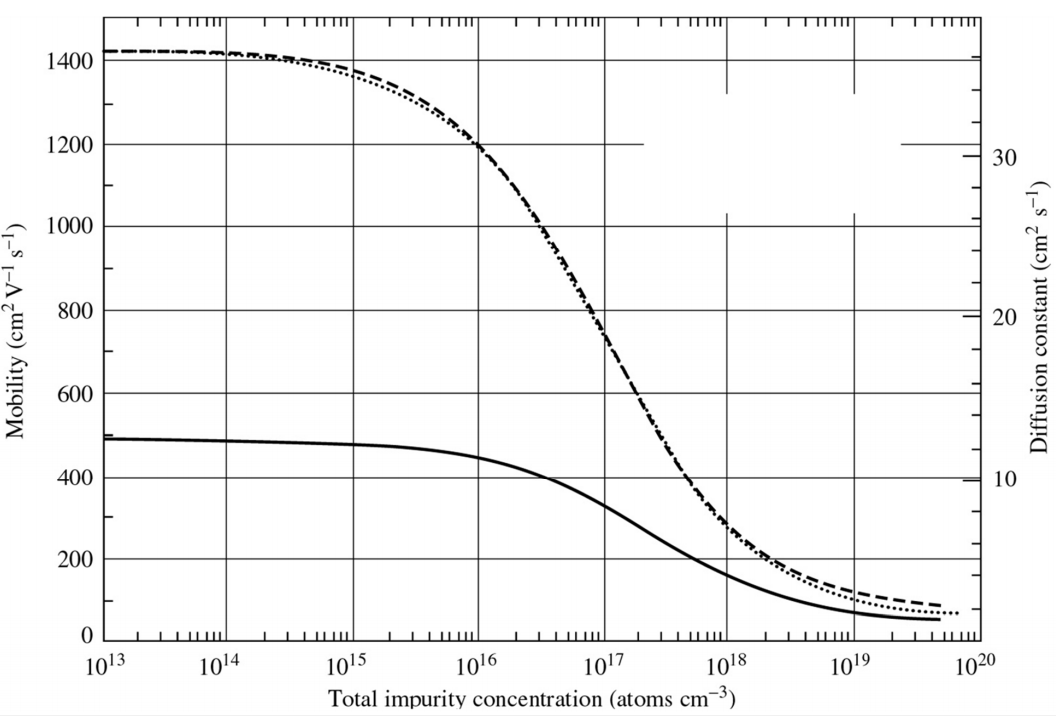
\includegraphics[width=1\linewidth]{DiffusionCoefficientChart.png}}
%\hspace{1em}
%\parbox[c]{4in}{\captionof{figure}{Diffusion Chart from Lecture I},
%\label{fig:pictureonright}}
%\end{minipage}

\begin{minipage}{\linewidth}
\centering
\raisebox{-.8in}{
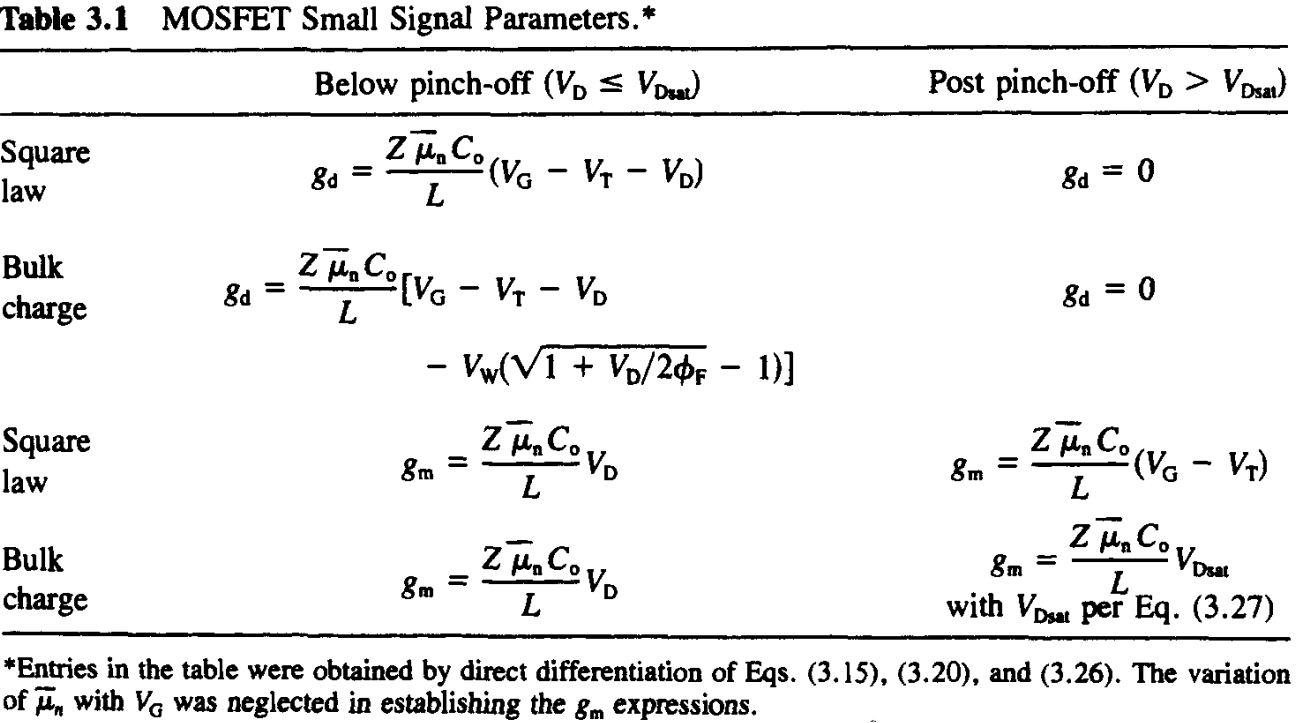
\includegraphics[width=1\linewidth]{MOSFETTable.png}}
\hspace{1em}
\parbox[c]{4in}{\captionof{figure}{Vol IV Mosfet table},
\label{fig:pictureonright}}
\end{minipage}
\begin{minipage}{\linewidth}
\centering
\raisebox{-.8in}{
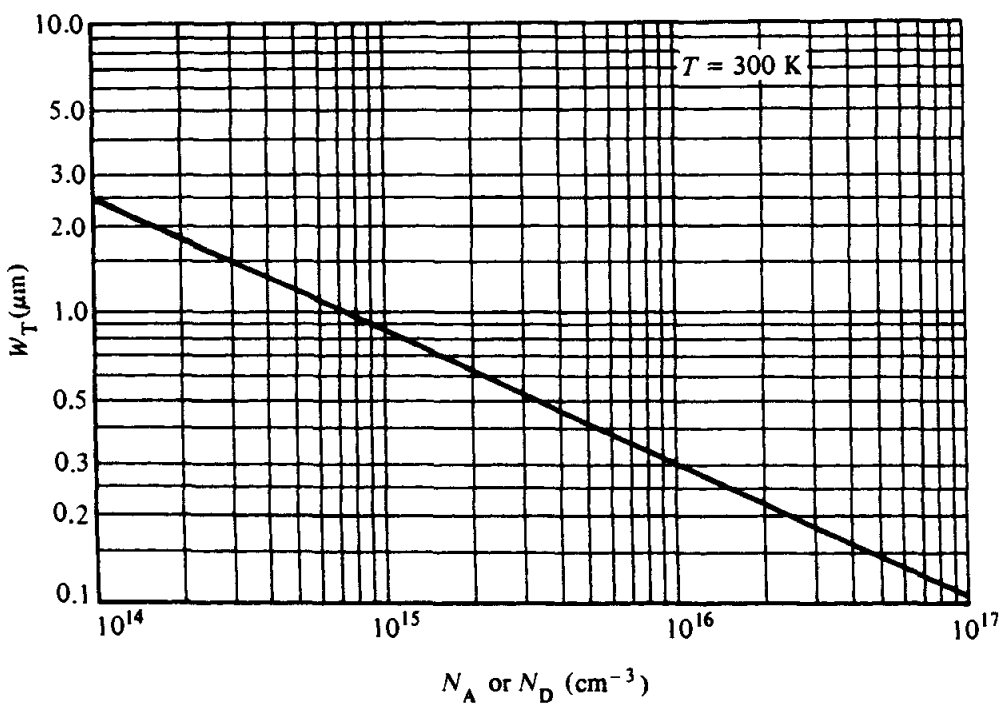
\includegraphics[width=1\linewidth]{MOSFETgraphdopants.PNG}}
\hspace{1em}
\parbox[c]{4in}{\captionof{figure}{Doping dependence of the maximum equilibrium depletion width inside silicon devices maintained at 300 K.},
\label{fig:pictureonright}}
\end{minipage}

\begin{minipage}{\linewidth}
	\centering
	\raisebox{-.8in}{
		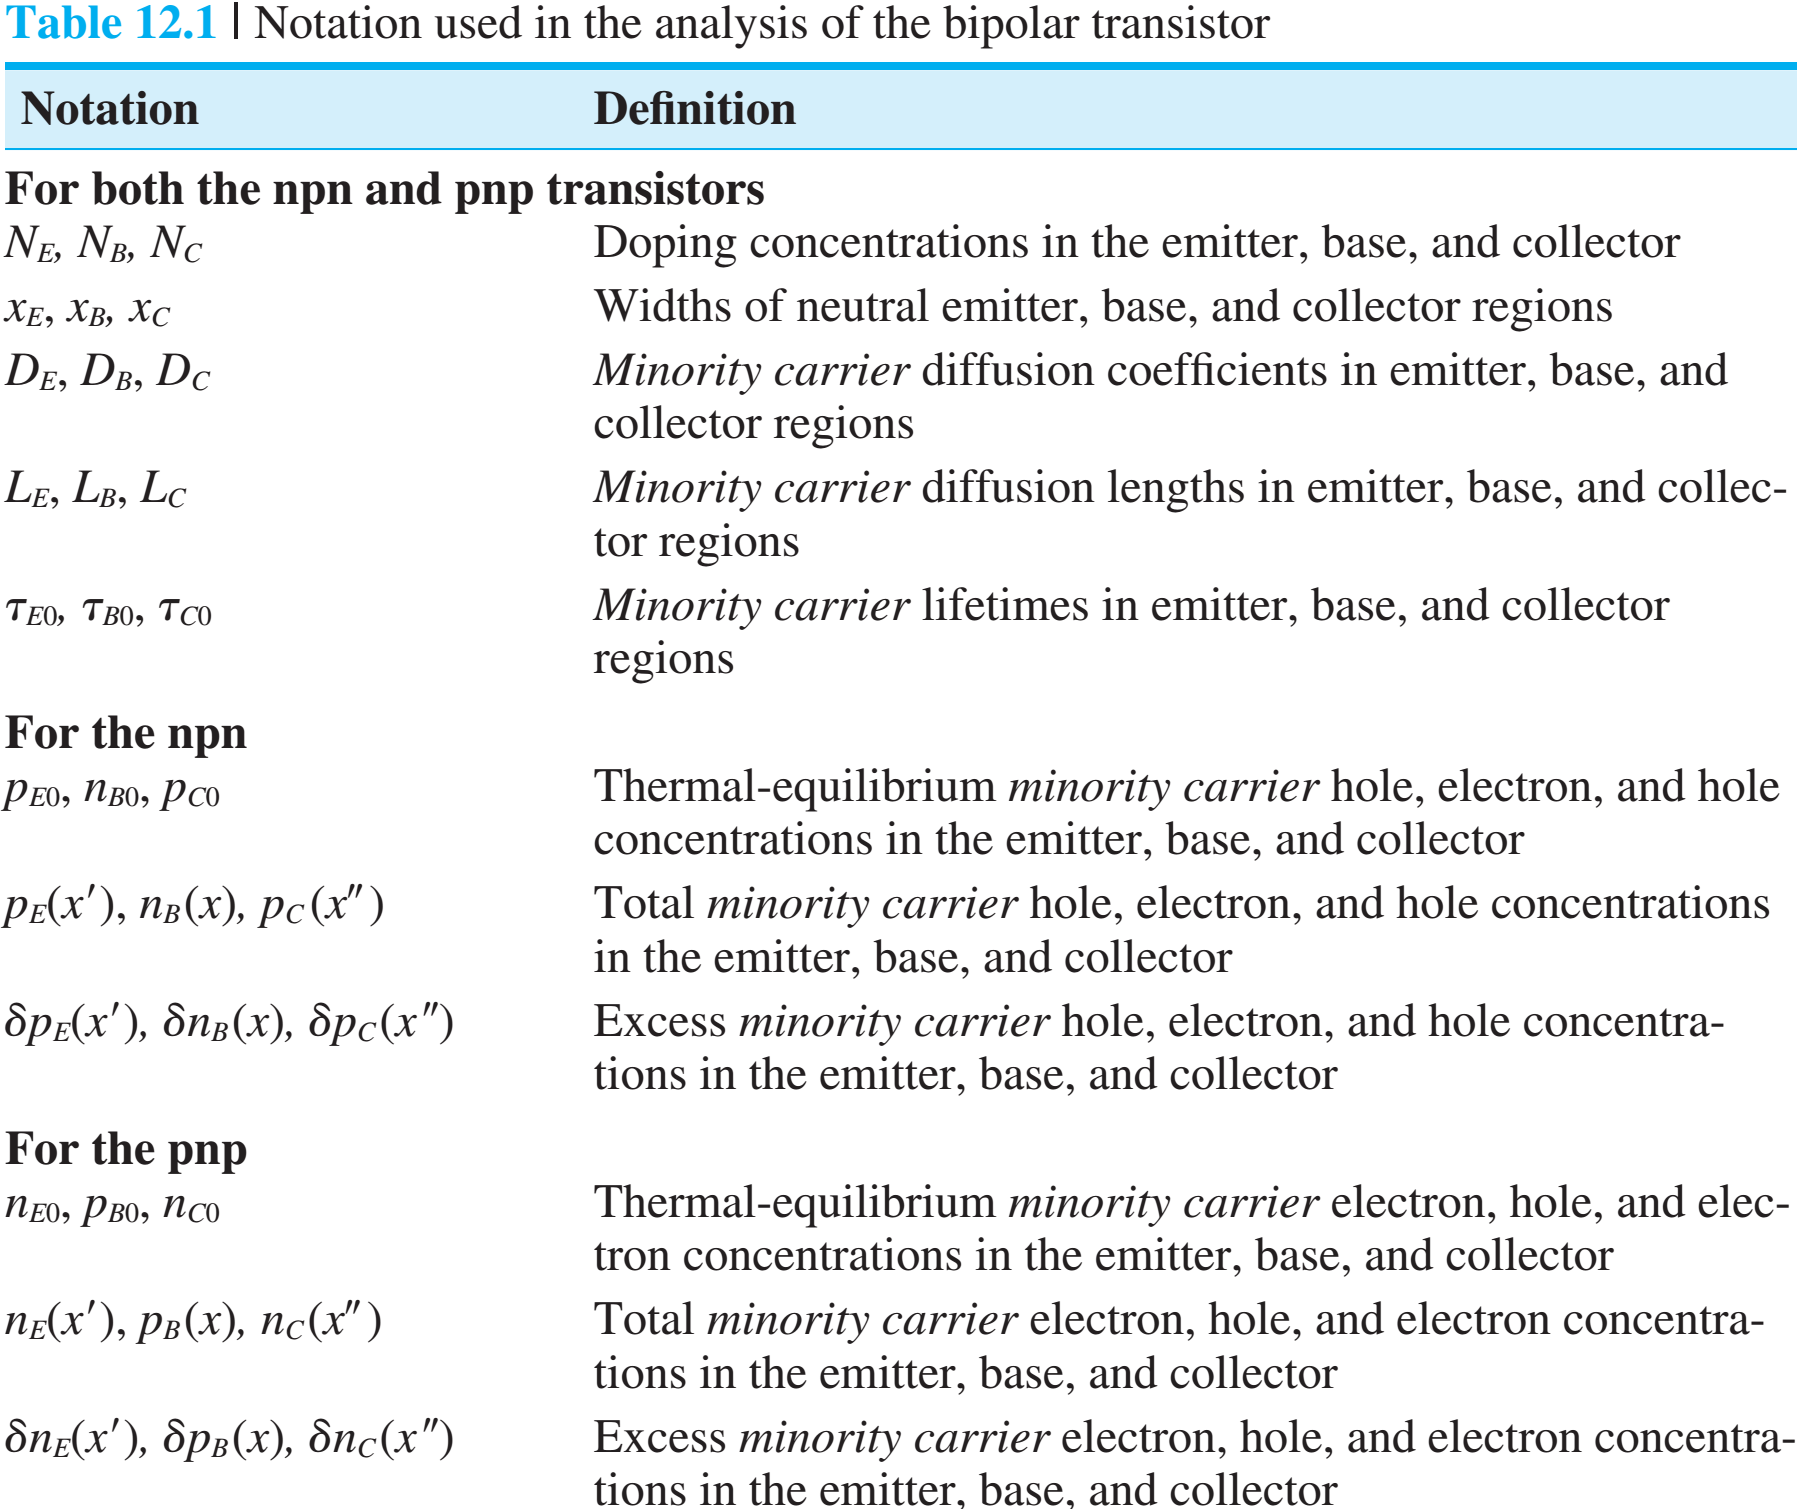
\includegraphics[width=1\linewidth]{NeamanTable12-1.png}}
	\hspace{1em}
	%\parbox[c]{4in}{\captionof{figure}{Resistivity Plot},
	\label{fig:pictureonrigh8194}
\end{minipage}
\begin{minipage}{\linewidth}
\centering
\raisebox{-.8in}{
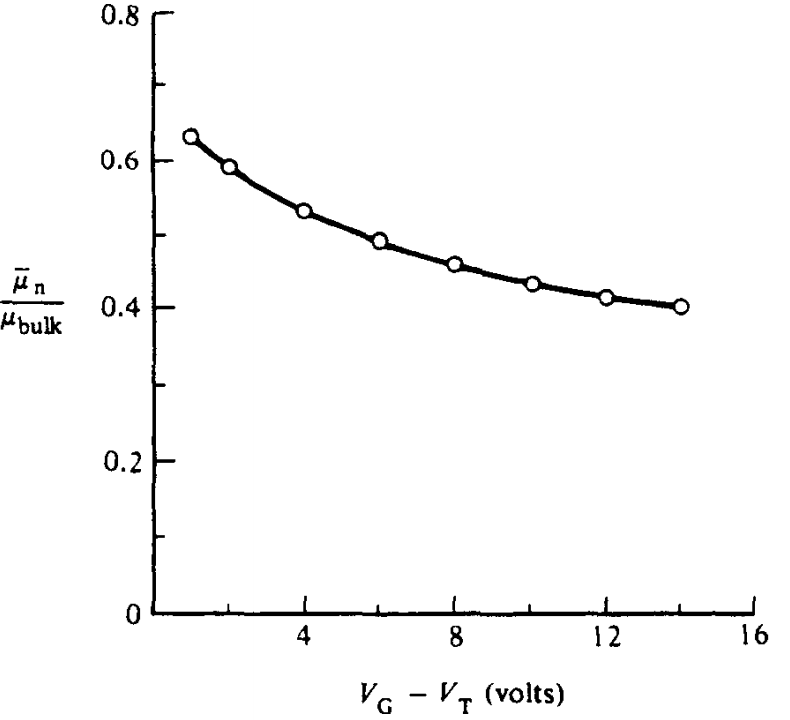
\includegraphics[width=0.6\linewidth]{MOSFETgraphVd_0.PNG}}
\hspace{1em}
\parbox[c]{4in}{\captionof{figure}{Vol IV Mosfet Gate voltages},
\label{fig:pictureonright}}
\end{minipage}

\begin{minipage}{\linewidth}
	\centering
	\raisebox{-.8in}{
		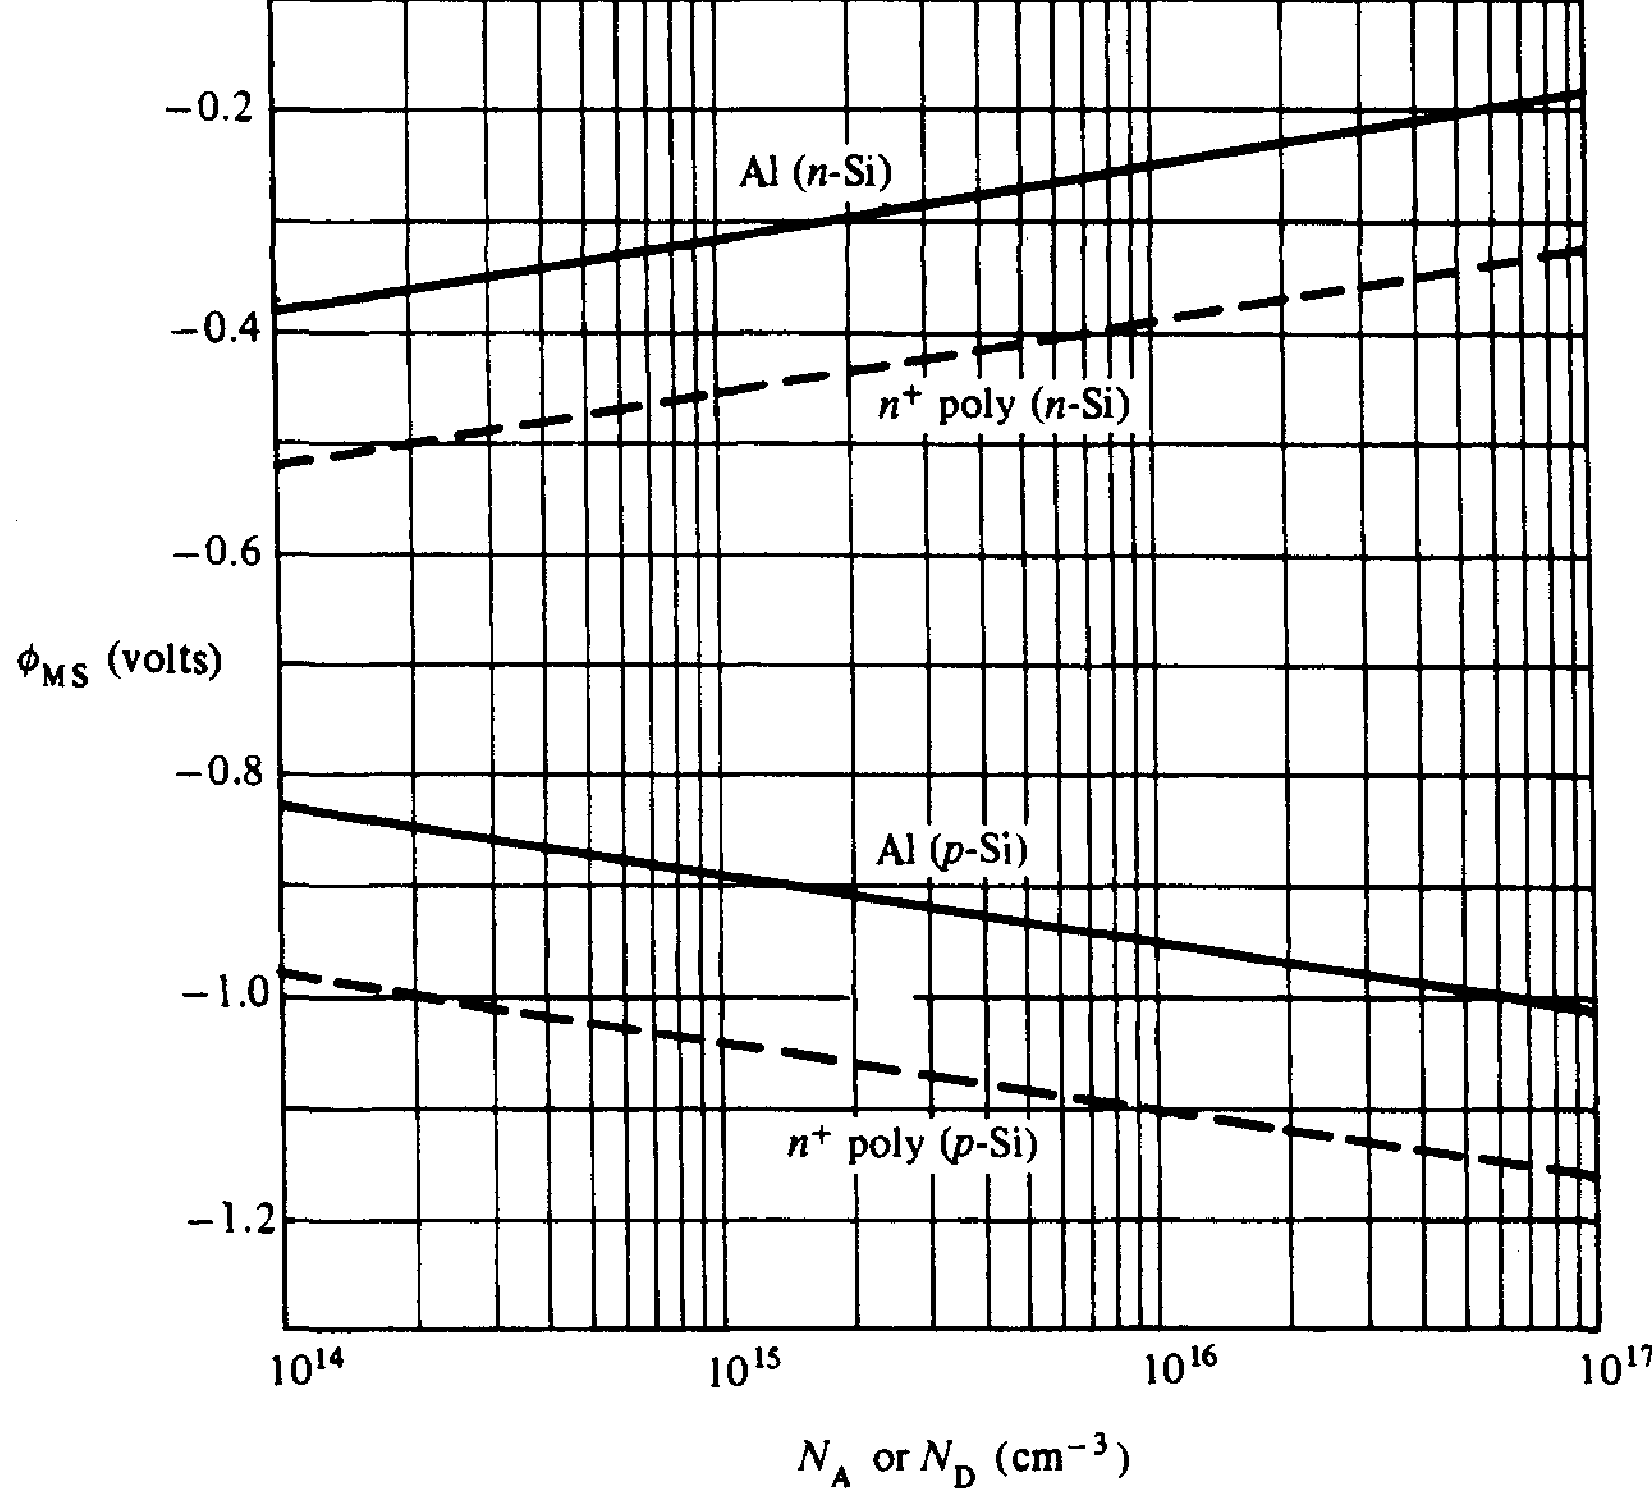
\includegraphics[width=1\linewidth]{Fig43VolIV.png}}
	\hspace{1em}
	\parbox[c]{4in}{\captionof{figure}{Workfunction difference as a function of a n- and p-type dopant conecntration in $n^+$ poly-Si-gate and Al-gate $SiO_2-Si$ structures. ($T=300 K$. $\phi_M^\prime-\chi^\prime=-0.18 \ eV$ for the $n^\prime$ poly-Si-gate structure; $\phi_M^\prime-\chi^\prime=0.03 eV$ for the Al-gate structure.)},
		\label{fig:pictureonright78}}
\end{minipage}
\begin{minipage}{\linewidth}
	\centering
	\raisebox{-.8in}{
		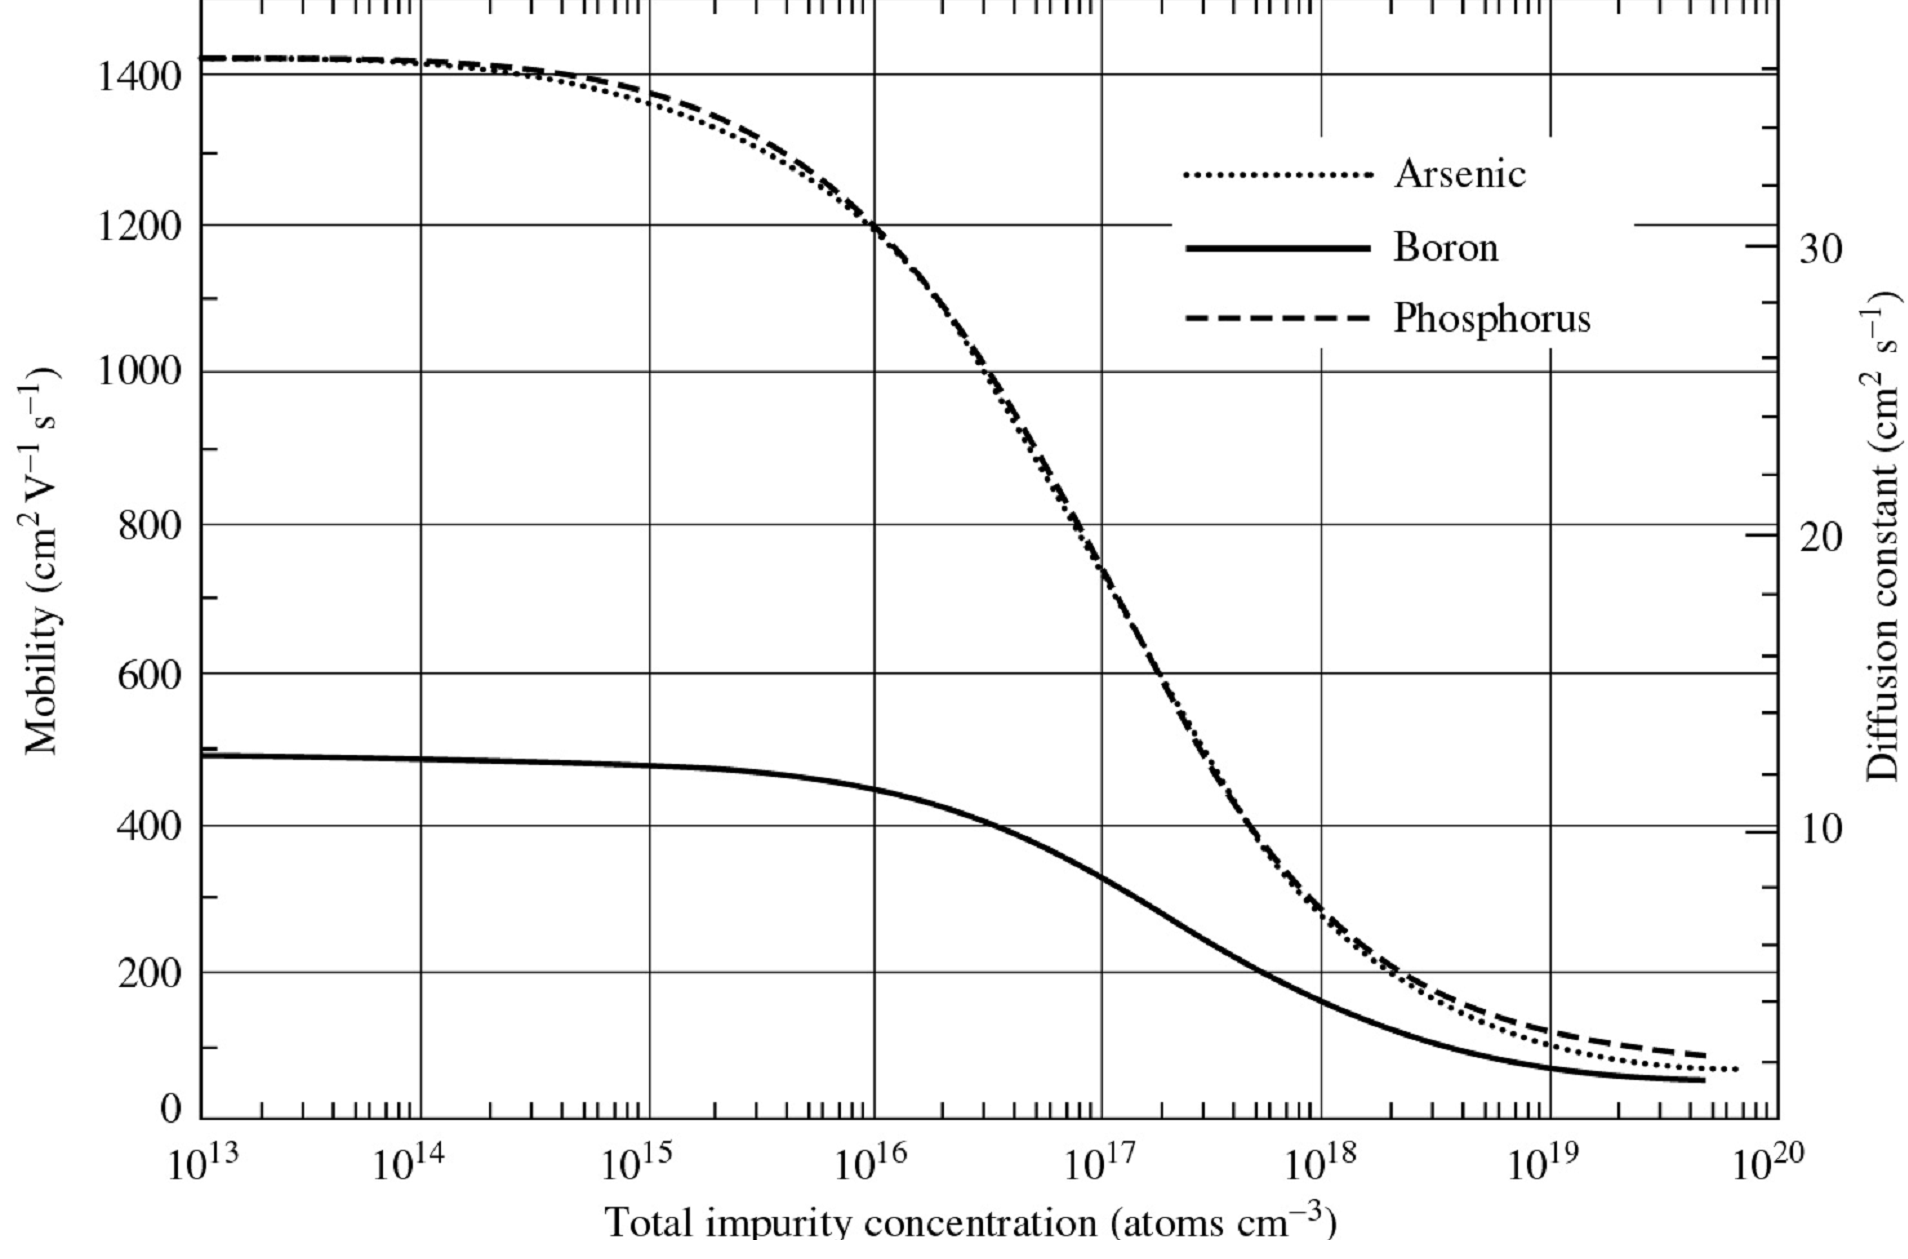
\includegraphics[width=0.7\linewidth]{GroupIIIGroupV.png}}
	%\hspace{1em}
%	\parbox[c]{4in}{\captionof{figure}{Boron Diffusion Chart},
		\label{fig:59}
\end{minipage}

\begin{minipage}{\linewidth}
	\centering
	\raisebox{-.8in}{
		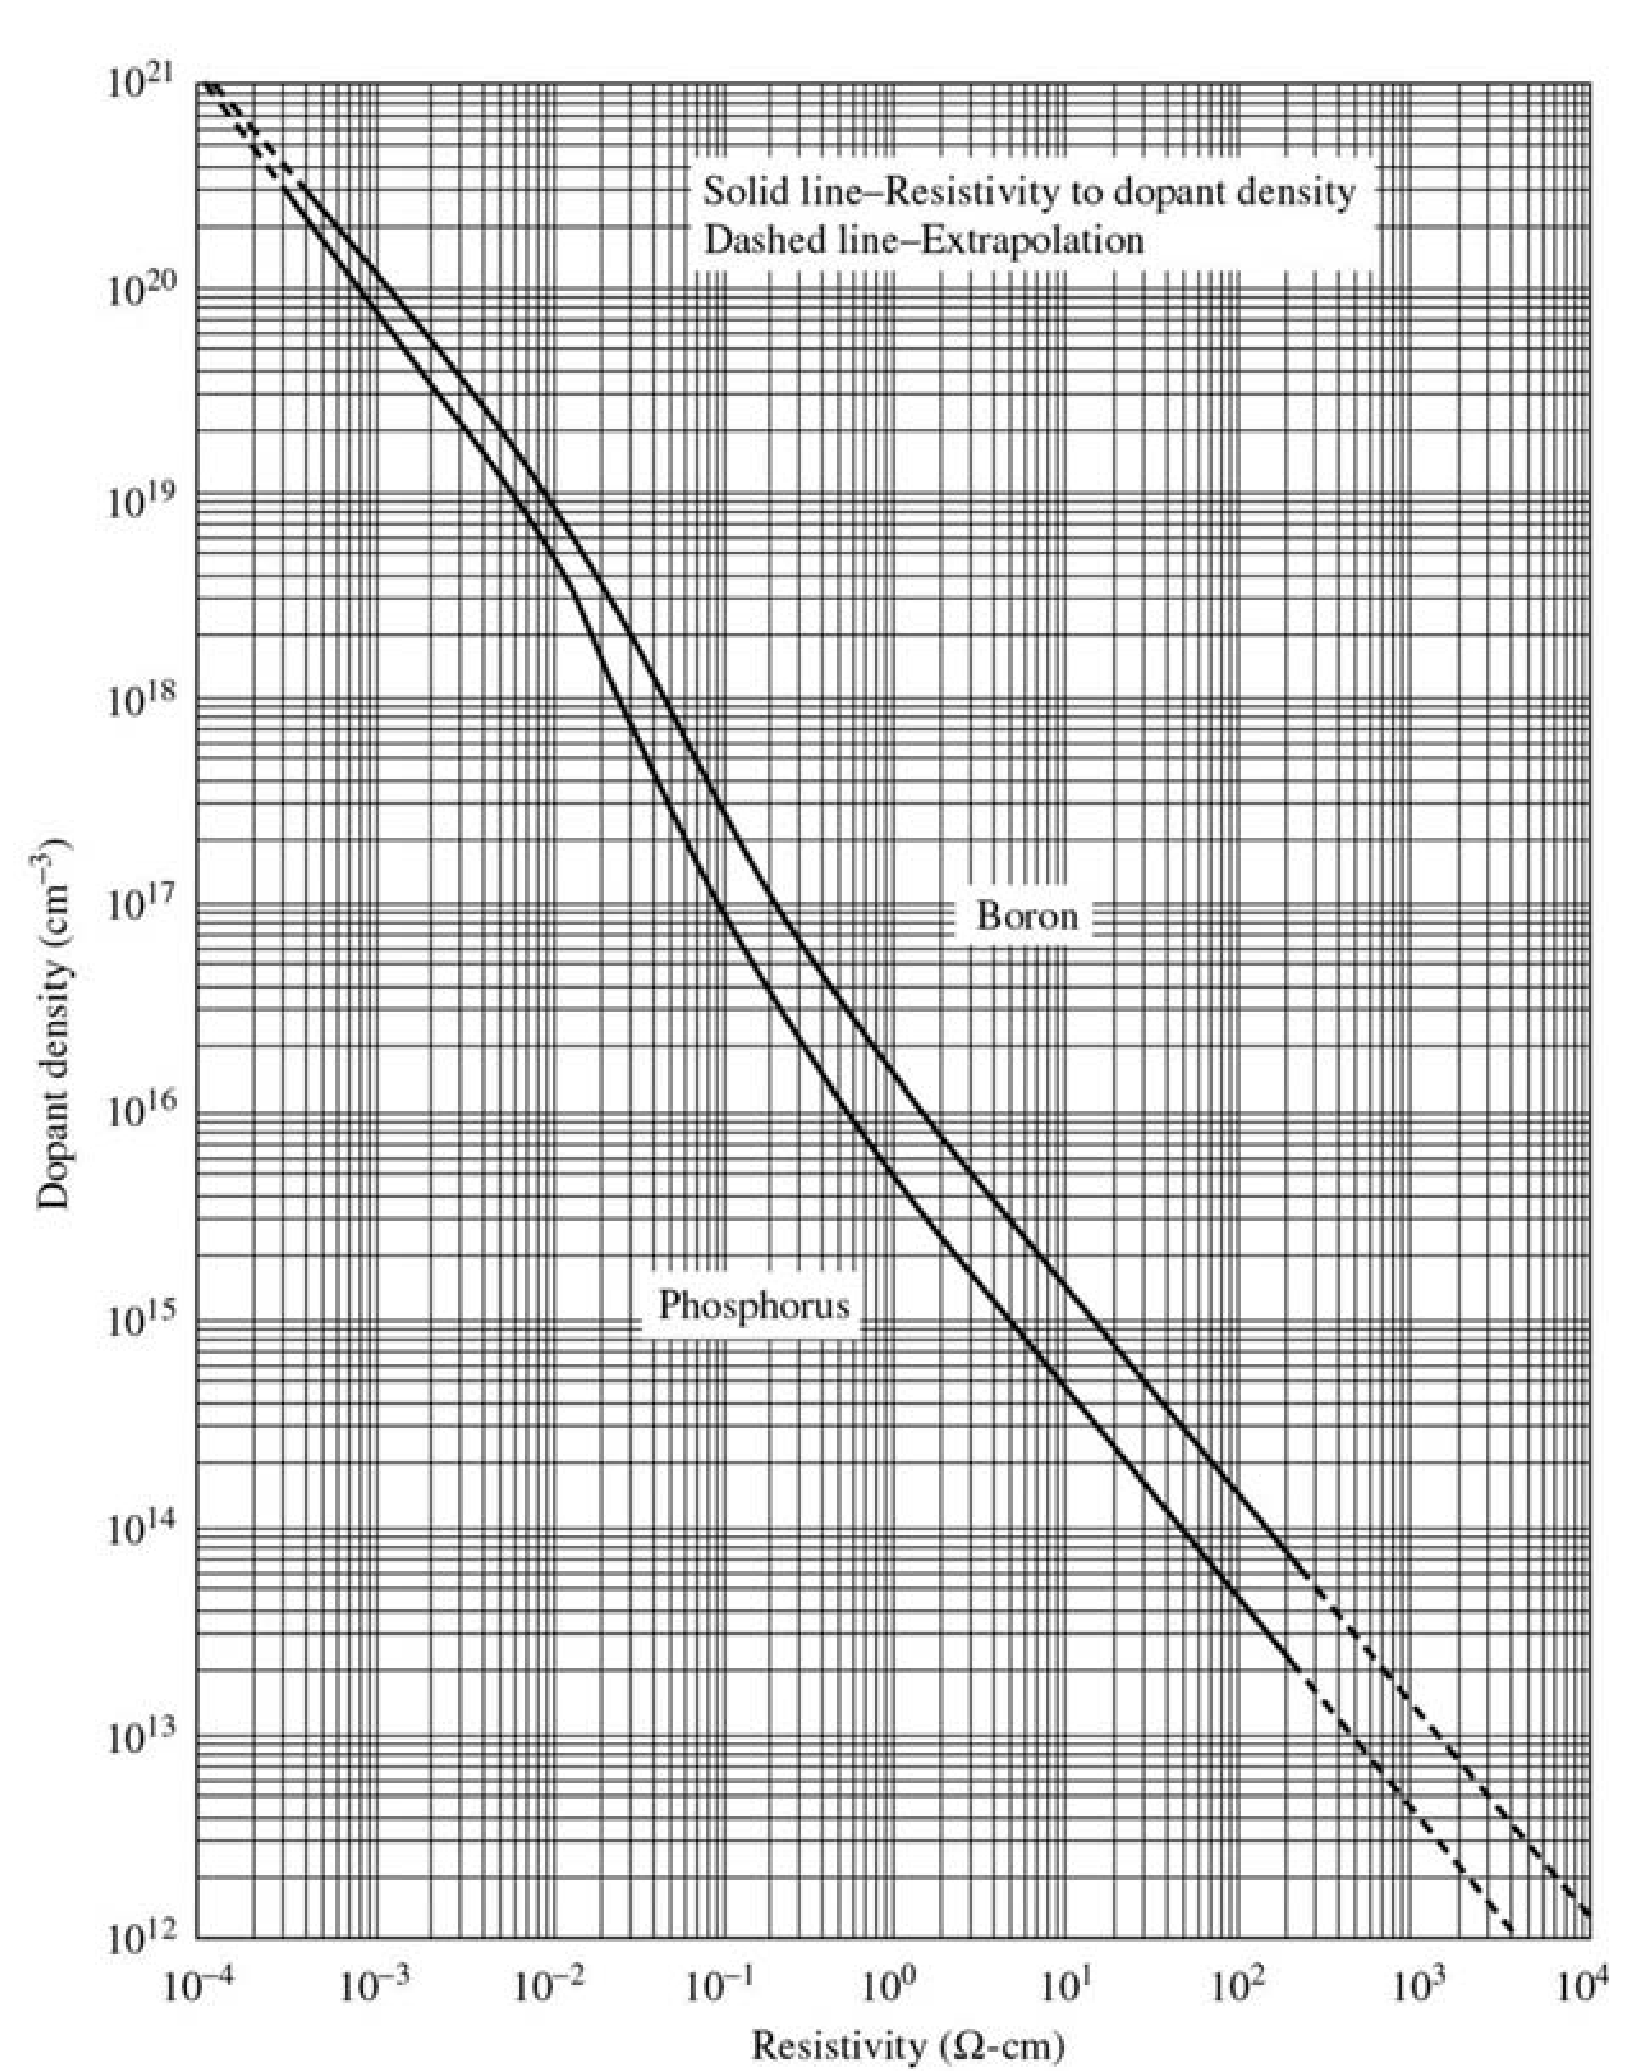
\includegraphics[width=0.7\linewidth]{boronChart.png}}
	\hspace{1em}
	\parbox[c]{4in}{\captionof{figure}{Boron Chart},
		\label{fig:4}}
\end{minipage}
\end{multicols}
\begin{minipage}{\linewidth}
	\centering
	\raisebox{-.8in}{
		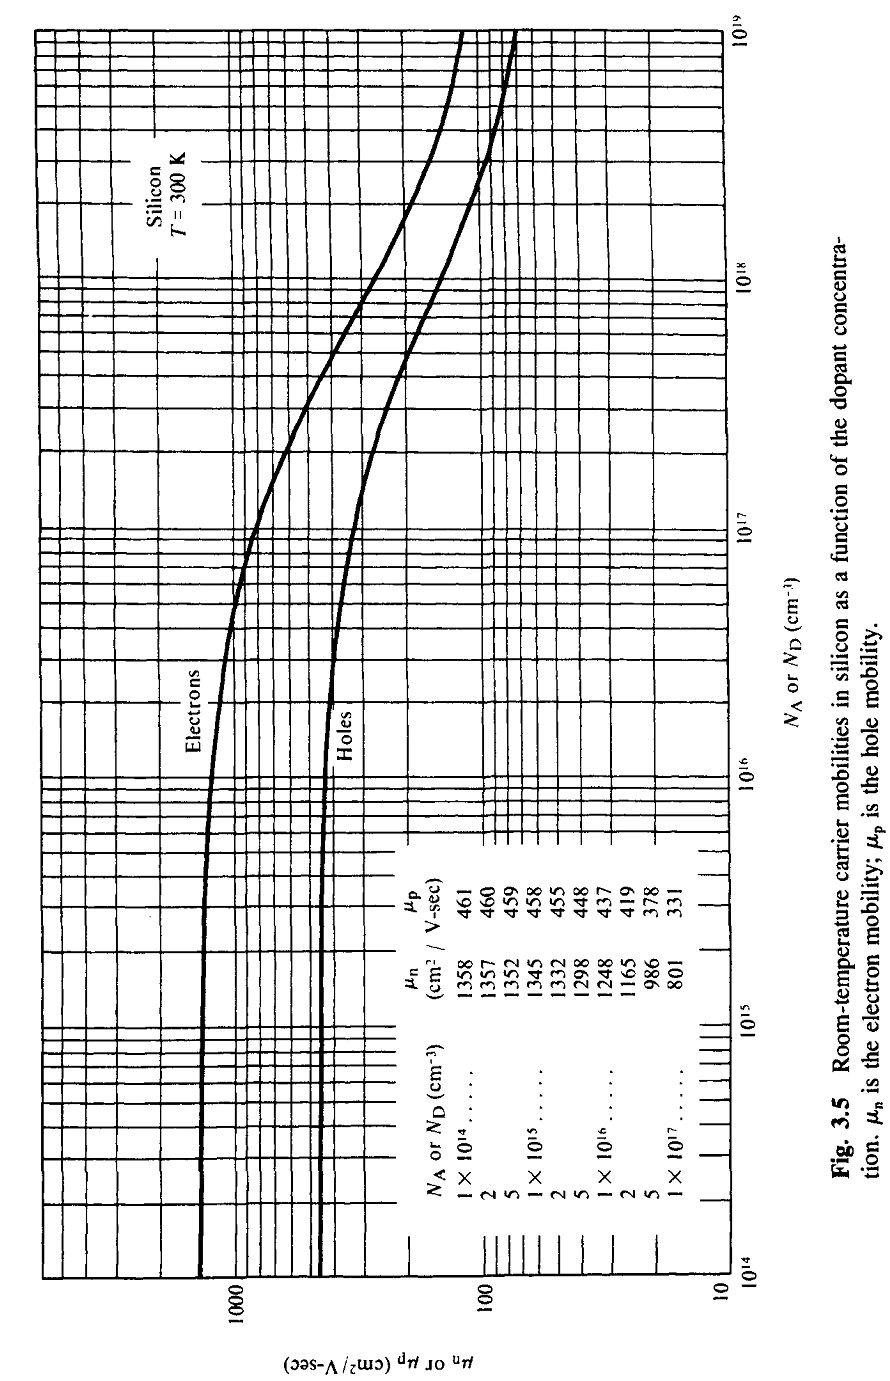
\includegraphics[height=1\textheight]{V1Figure3-5.png}}
% 	\hspace{1em}
% 	\parbox[c]{4in}{\captionof{figure}{Diffussion Constant},
% 		\label{fig:pictureonright79}}
\end{minipage}

\begin{minipage}{\linewidth}
	\centering
	\raisebox{-.8in}{
		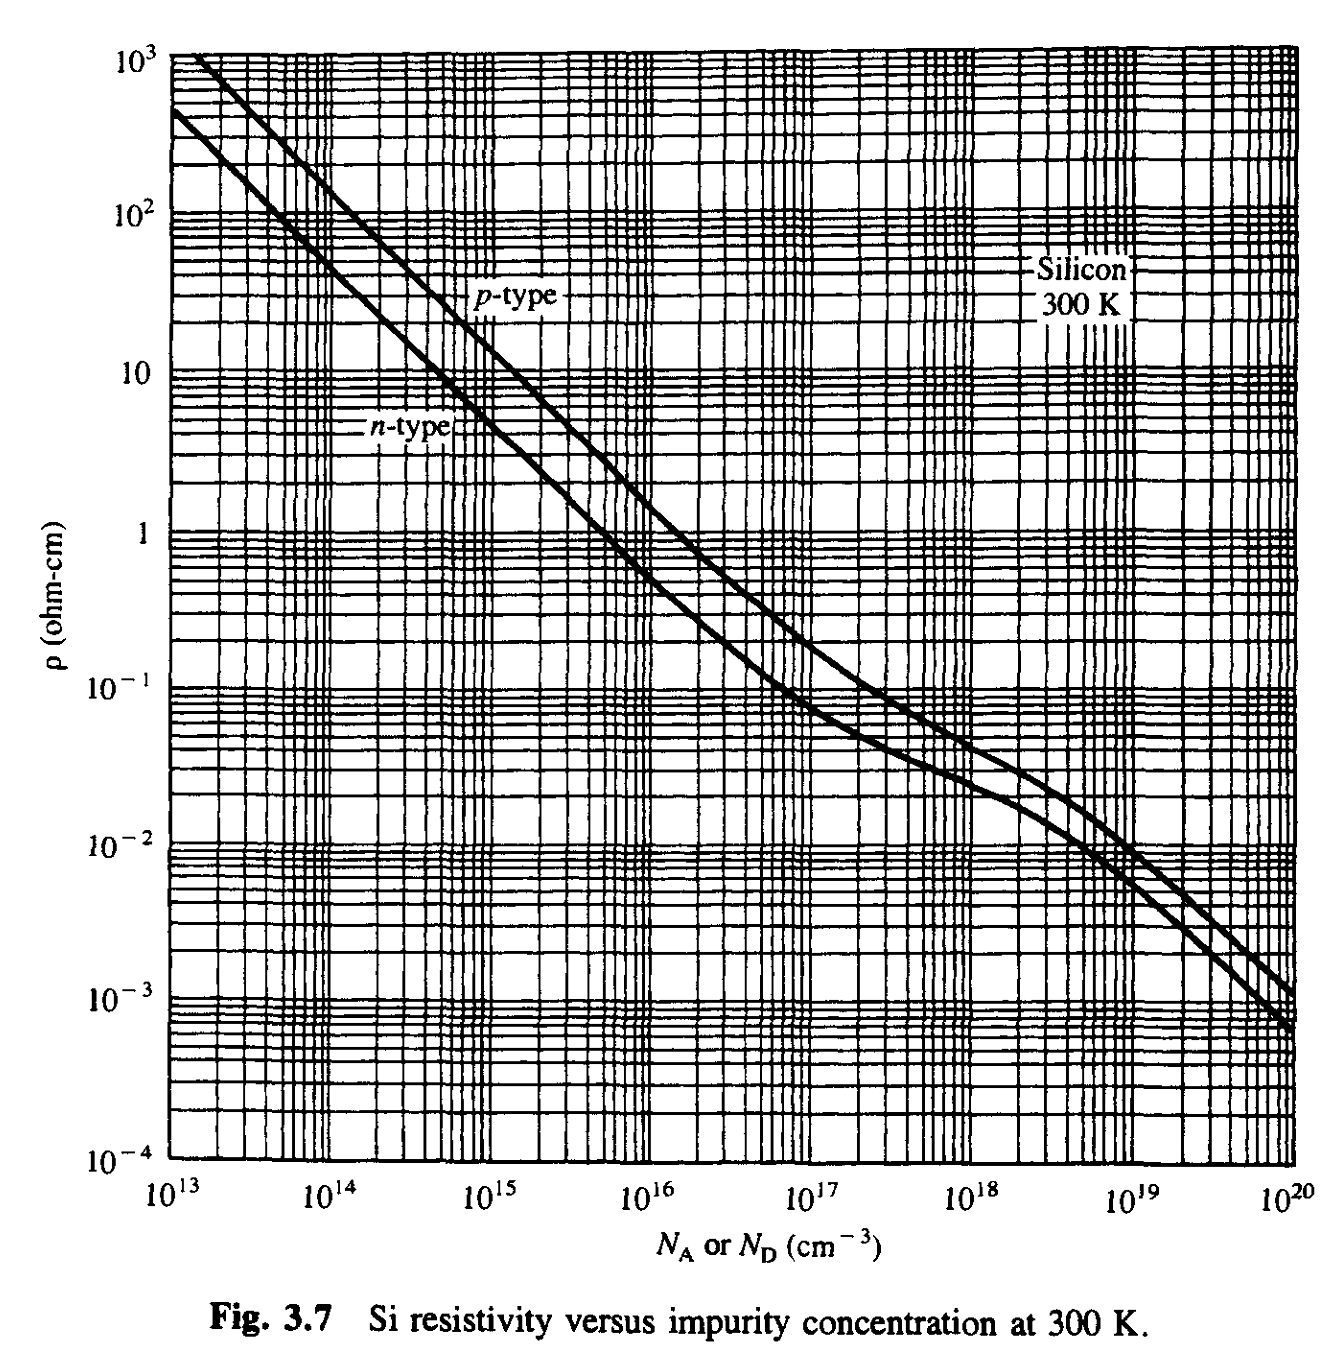
\includegraphics[width=1\textheight]{VIFigure3-7.png}}
	\hspace{1em}
	%\parbox[c]{4in}{\captionof{figure}{Resistivity Plot},
		\label{fig:pictureonrigh819}
\end{minipage}
%% Added this section, to ha ve a list of algorithms in lwarp
\chapter{CENG242Cheat}
\todo{Remember to add more algorithms later}{Future Work}

\begin{algorithm}
\caption{Euclid’s algorithm}\label{euclid}
\begin{algorithmic}[1]
\Procedure{Euclid}{$a,b$}\Comment{The g.c.d. of a and b}
\State $r\gets a\bmod b$
\While{$r\not=0$}\Comment{We have the answer if r is 0}
\State $a\gets b$
\State $b\gets r$
\State $r\gets a\bmod b$
\EndWhile\label{euclidendwhile}
\State \textbf{return} $b$\Comment{The gcd is b}
\EndProcedure
\end{algorithmic}
\end{algorithm}



 \begin{algorithm}
	\caption{Merge Sort}
	\begin{algorithmic}[1]
		\Function{Merge}{$A,p,q,r$}\Comment{Where A - array, p - left, q - middle, r - right}
		
		\State ${n_1} = q - p + 1$
		\State ${n_2} = r - q$
		\State Let $L[1 \ldots {n_1} + 1]$ and $R[1 \ldots {n_2} + 1]$ be new arrays
		\For{$i = 1$ to ${n_1}$}
		\State $L[i] = A[p + i - 1]$
		\EndFor
		\For{$j = 1$ to ${n_2}$}
		\State $R[i] = A[q + j]$
		\EndFor
		\State $L[{n_1} + 1] =  \infty $
		\State $R[{n_2} + 1] =  \infty $
		\State $i = 1$
		\State $j = 1$
		\For{$k = p$ to $r$}
		\If {$L[i] < R[j]$}
		\State $A[k] = L[i]$
		\State $i = i + 1$
		\ElsIf {$L[i] > R[j]$}
		\State $A[k] = R[j]$
		\State $j = j + 1$
		\Else
		\State $A[k] = - \infty$ \Comment{We mark the duplicates with the largest negative integer}
		\State $j = j + 1$
		\EndIf
		\EndFor
		\EndFunction
		
	\end{algorithmic}
\end{algorithm}

\section{Basic Graph Definitions}
\begin{itemize}
	\item A graph $G = (V,E)$ consists of a finite set of {\em vertices} $V$
	and a finite set of {\em edges} $E$.
	\begin{itemize}
		\item {\em Directed graphs}: $E$ is a set of ordered pairs of vertices
		$(u,v)$ where $u,v \in V$ \\
		% \centerline{\epsfig{file=directed_example.eps,height=3.5cm}}
		\item {\em Undirected graph}: $E$ is a set of unordered pairs of
		vertices $\{u,v\}$ where $u,v \in V$ \\ \\
		% \centerline{\epsfig{file=undirected_example.eps,height=3cm}}
	\end{itemize}
	\item Edge $(u,v)$ is {\em incident} to $u$ and $v$
	\item {\em Degree} of vertex in undirected graph is the number of edges
	incident to it.
	\item {\em In (out) degree} of a vertex in directed graph is the number of
	edges entering (leaving) it.
	\item A {\em path} from $u_1$ to $u_2$ is a sequence of vertices
	$<u_1$=$v_0,v_1,v_2, \cdots , v_k$=$u_2>$ such that $(v_i,v_{i+1}) \in E$
	(or $\{v_i,v_{i+1}\} \in E$)
	\begin{itemize}
		\item We say that $u_2$ is {\em reachable} from $u_1$
		\item The {\em length} of the path is $k$
		\item It is a {\em cycle } if $v_0 = v_k$
	\end{itemize}
	
	
	\item An undirected graph is {\em connected /} if every pair of vertices are
	connected by a path
	\begin{itemize}
		\item The {\em connected components } are the equivalence classes of
		the vertices under the ``reachability'' relation. (All connected
		pair of vertices are in the same connected component).
	\end{itemize}
	\item A directed graph is {\em strongly connected } if every pair of
	vertices are reachable from each other
	\begin{itemize}
		\item The {\em strongly connected components } are the equivalence
		classes of the vertices under the ``mutual reachability'' relation. 
	\end{itemize}
	
	\vspace*{\baselineskip}
	
	\item Graphs appear all over the place in all kinds of applications, e.g:
	\begin{itemize}
		\item Trees $(\vert E \vert = \vert V \vert - 1)$
		\item Connectivity/dependencies (house building plans, WWW-page
		connections = internet graph)
	\end{itemize}
	\item Often the edges $(u,v)$ in a graph have weights $w(u,v)$, e.g.
	\begin{itemize}
		\item Road networks (distances)
		\item Cable networks (capacity)
	\end{itemize}
\end{itemize}


\subsection{Representation}
\begin{itemize}
	\item {\em Adjacency-list} representation:
	\begin{itemize}
		\item Array of $\vert V \vert$ list of edges incident to each
		vertex. \\
		
		Examples: \\
		\item Note: For undirected graphs, every edge is stored twice.
		\item If graph is weighted, a weight is stored with each edge.
	\end{itemize}
	
	
	\item {\em Adjacency-matrix} representation:
	\begin{itemize}
		\item $\vert V \vert \times \vert V \vert$ matrix $A$ where 
		\[ a_{ij} = \left\{ \begin{array}{ll}
		1        & \mbox{ if $(i,j) \in E$} \\
		0        & \mbox{ otherwise } \\
		\end{array}
		\right. \]
		
		Examples: \\
		\item Note: For undirected graphs, the adjacency matrix is
		symmetric along the main diagonal ($A^T = A$).
		\item If graph is weighted, weights are stored instead of one's.
	\end{itemize}
	\item Comparison of matrix and list representation: \\
	\begin{itemize}
		\item[]
		\begin{tabular}{l|l}
			Adjacency list & Adjacency matrix \\ \hline
			$O(\vert V \vert + \vert E \vert)$ space & $O(\vert V \vert ^2)$
			space \\
			Good if graph {\em sparse} $(\vert E \vert << \vert V
			\vert ^2)$ & Good if graph {\em dense} $(\vert E \vert \approx
			\vert V \vert ^2)$ \\
			No quick access to $(u,v)$ & $O(1)$ access to $(u,v)$ \\
		\end{tabular}
	\end{itemize}
	\item We will use adjacency list representation unless stated otherwise
	($O(|V|+|E|)$ space).
\end{itemize}


\section{Graph traversal}
\begin{itemize}
	\item There are two standard (and simple) ways of traversing all
	vertices/edges in a graph in a systematic way
	\begin{itemize}
		\item Breadth-first
		\item Depth-first
	\end{itemize}
	\item We can use them in many fundamental algorithms, e.g finding cycles,
	connected components, $\dots$
\end{itemize}

\subsection{Breadth-first search (BFS)}
\begin{itemize}
	\item Main idea:
	\begin{itemize}
		\item Start at some source vertex $s$ and visit,
		\item All vertices at distance 1,
		\item Followed by all vertices at distance 2,
		\item Followed by all vertices at distance 3,
		
		$\vdots$
	\end{itemize}
	\item BFS corresponds to computing {\em shortest path} distance (number of
	edges) from $s$ to all other vertices.
	\item To control progress of our BFS algorithm, we think about {\em coloring}
	each vertex
	\begin{itemize}
		\item {\em White } before we start,
		\item {\em Gray } after we visit the vertex but before we have
		visited all its adjacent vertices,
		\item {\em Black } after we have visited the vertex and all its
		adjacent vertices (all adjacent vertices are gray).
	\end{itemize}
	\item We use a queue $Q$ to hold all gray vertices---vertices we have seen
	but  are still not done with.
	\item We remember from which vertex a given vertex $v$ is colored gray
	-- i.e. the node that discovered $v$ first; this is called
	parent[$v$].
	\item Algorithm: \\ \\
	\fbox{
		\parbox{10cm}{
			{\sc BFS($s$) }
			\begin{itemize}
				\item[] color[$s$] = gray
				\item[] $d[s] = 0$
				\item[] ENQUEUE($Q,s$)
				\item[] WHILE $Q$ not empty DO
				\begin{itemize}
					\item[] DEQUEUE($Q,u$)
					\item[] FOR $(u,v)\in E$ DO
					\begin{itemize}
						\item[] IF color[$v$] = white THEN
						\item[] ~~~~color[$v$] = gray
						\item[] ~~~~$d[v] = d[u] + 1$
						\item[] ~~~~parent[$v$] = u
						\item[] ~~~~ENQUEUE($Q,v$)
						\item[] FI
						\item[] color[$u$] = black
					\end{itemize}
				\end{itemize}
				\item[] OD
			\end{itemize}
	}}
	\vspace*{\baselineskip}
	
	\item Algorithm runs in $O(\vert V \vert + \vert E \vert)$ time
	
	
	\item Example (for directed graph): \\
	\item Note:
	\begin{itemize}
		\item parent[$v$] forms a tree; {\em BFS-tree}.
		\item $d[v]$ contains length of shortest path from $s$ to
		$v$. (Prove by induction)
		\item We can use parent[$v$] to find the shortest path from $s$ to a
		given vertex.
		%       \item We can use algorithm to detect cycles; just check if gray
		%       node is ever met.
	\end{itemize}
	\item If graph is not connected we have to try to start the traversal
	at all nodes. \\
	
	\fbox{
		\parbox{8cm}{ 
			FOR each vertex $u \in V $ DO
			\begin{itemize}
				\item[] IF color[$u$] = white THEN BFS($u$)
			\end{itemize}
			OD
	}}
	
	\begin{itemize}
		\item Note: We can use algorithm to compute connected components in
		$O(|V|+|E|)$ time.
	\end{itemize}
\end{itemize}



\subsection{Depth-first search (DFS)}
\begin{itemize}
	\item If we use stack instead of queue $Q$ we get another traversal order;
	depth-first
	\begin{itemize}
		\item We go ``as deep as possible'',
		\item Go back until we find unexplored adjacent vertex,
		\item Go as deep as possible,
		
		$\vdots$
	\end{itemize}
	\item Often we are interested in ``start time'' and ``finish time'' of
	vertex $u$
	\begin{itemize}
		\item {\em Start time\/} (d[$u$]): indicates at what ``time'' vertex
		is first visited.
		\item {\em Finish time\/} (f[$u$]): indicates at what ``time'' all
		adjacent vertices have been visited.
	\end{itemize}
	\item We can write DFS iteratively using the same algorithm as for BFS
	but with a STACK instead of a QUEUE, or, we can write a recursive DFS
	procedure
	\begin{itemize}
		\item We will color a vertex gray when we first meet it and black
		when we finish processing all adjacent vertices.
	\end{itemize}
	\item Algorithm: \\
	
	\fbox{
		\parbox{8cm}{
			{\sc DFS($u$) } 
			\begin{itemize}
				\item[] color[$u$] = gray
				\item[] $d[u]$ = time
				\item[] time = time + 1
				\item[] FOR $(u,v)\in E$ DO
				\begin{itemize}
					\item[] IF color[$v$] = white THEN
					\begin{itemize}
						\item[] parent[$v$] = $u$
						\item[] {\sc DFS(v)}
					\end{itemize}
					\item[] FI
				\end{itemize}
				\item[] OD
				\item[] color[$u$] = black
				\item[] $f[u]$ = time
				\item[] time = time + 1
			\end{itemize}
	}}
	
	\item Algorithm runs in $O(\vert V \vert + \vert E \vert)$ time
	\begin{itemize}
		\item As before we can extend algorithm to unconnected graphs and
		we can use it to detect cycles in $O(|V|+|E|)$ time.
	\end{itemize}
	
	\item As previously parent[$v$] forms a tree; {\em DFS-tree}
	\begin{itemize}
		\item Note: If $u$ is descendent of $v$ in DFS-tree  then $d[v] <
		d[u] < f[u] < f[v]$
	\end{itemize}
\end{itemize}

%%%%%%%%%%%%%%%%%%%%%%%%%%%%%%%%%%%%%%%%%%%%%%%%%%%%%%%%%%%%%%%%%%%%%%


\section{Topological sorting}
\begin{itemize}
	\item Definition: Topological sorting of {\em directed acyclic graph}
	$G=(V,E)$ is a linear ordering of vertices $V$ such that $(u,v) \in E
	\Rightarrow u$ appear before $v$ in ordering.
	\item Topological ordering can be used in scheduling:
	\begin{itemize}
		\item Example: Dressing (arrow implies ``must come before'') \\ \\
		% \centerline{\epsfig{file=top_sort_example.eps,height=5.5cm}} \\
		
		We want to compute order in which to get dressed. One possibility: \\
		
		
		\vspace*{\baselineskip}
		
		The given order is one possible topological order.
	\end{itemize}
	\item Algorithm: Topological order just reverse DFS finish time ($
	\Rightarrow O(\vert V \vert + \vert E \vert)$ running time).
	\item Correctness: $(u,v) \in E \Leftrightarrow f(v) < f(u)$
	\begin{itemize}
		\item Proof: When $(u,v)$ is explored by DFS algorithm, $v$ must be
		white or black (gray $\Rightarrow$ cycle).
		\begin{itemize}
			\item $v$ white: $v$ visited and finished before $u$ is
			finished $\Rightarrow f(v) < f(u)$
			\item $v$ black: $v$ already finished $\Rightarrow f(v) <
			f(u)$
		\end{itemize}
	\end{itemize}
	\item Alternative algorithm: Count in-degree of each vertex and repeatedly
	number and remove in-degree 0 vertex and its outgoing edges: Homework. 
	
\end{itemize}

\chapter{ELEC 220 CheatSheet}
\begin{multicols}{3}

\section{Ch.1 DC Conduction}
$\sigma$ = conductivity (S/m) and $ \rho$ = resistivity ($ \Omega $m). $\sigma = 1 /\ \rho $. 
\begin{table}
\begin{tabular}{c|c}
	Hall coefficient    & $R_H= \frac{v_D}{J}=\frac{-1}{eN_e}=(-eN_e)^{-1}$ \\
	Ohm's Law  & $J = \sigma \cdot E \quad A /\ m^{2}$\\ 
	Resistance & $R= \frac{\rho \cdot  L}{A}= \frac{L}{\sigma \cdot A}$ \\
	Drude Model  & $J = -eN_ev_D$ \\
	Viscosity Model  & $v_D=\frac{-e\tau}{m_e}E$
\end{tabular}
\caption{Some Equations for DC Conduction}
\end{table}
$$\textbf{Scattering time Formula:} \quad \sigma= \frac{e^2N_e\tau}{m_e} $$

\section{Ch. 2 AC Conduction}
\begin{align} 
\textbf{Skin Depth:} \quad \delta= 
\left(\frac{2}{\omega \mu \sigma}\right)^{1/2} \\
E= E_0e^{-i(wt-z/\ \delta)}e^{-z/\ \delta} \\
I \sim e^{-2z /\ \delta} \\
I \propto |E|^{2} \\
\omega = \frac{2\pi c}{\lambda_o}
\end{align} 
\begin{align} 
\textbf{Plasma Frequency:} \quad \omega_p= 
\left(\frac{N_ee^2}{m \epsilon}\right)^{1/2} \\
k^2= \omega^2 \mu \epsilon - \frac{N_ee^2\mu}{m}= \omega^2\mu\epsilon\left(1-\frac{\omega_p^2}{\omega^2}\right)
\end{align} 
%\def\bsq#1{%both single quotes
%	\lq{#1}\rq}
\section{Ch. 3 DC/AC Dielectrics}
\begin{align} 
\textbf{Relative Permittivity:} \quad = \frac{C^\prime}{C}=\frac{Q^\prime}{Q}
= \epsilon_r \\
PA=Q^\prime - Q = C^\prime V - CV= CV(\epsilon_r-1) \\
P= \epsilon_0E(\epsilon_r-1) \ and \ \epsilon_r=1+\frac{P}{\epsilon_0E}= 1+\chi \\
D = \epsilon E = \epsilon_0 \epsilon_r E = \epsilon_0 E+ P \\
P = Np = Nqd \\
\epsilon_= 1 + \frac{N \alpha_e}{\epsilon_0}=1+\chi
\end{align}
\begin{align}
\textbf{Debye Model:} \quad 
\epsilon_d(\omega)= \frac{\epsilon_d(0)}{1-i\omega \tau_r}=\epsilon_d^\prime+i\epsilon_d^{\prime \prime}\\
\epsilon_d^\prime= \frac{\epsilon_d(0)}{1+\omega^2 \tau_r^2} \quad and \quad \epsilon_d^{\prime \prime}(\omega)= \frac{\epsilon_d(0)}{1+\omega^2 \tau_r^2}\omega \tau_r
\end{align}
Different Polarization Mechanisms(Decreasing Speed)
Electronic	\\
Ionic	\\
Dipolar (Orientational)	\\
Space Charge (Interfacial)	\\
Ferroelectric
\section{Ch. 4 AC Dielectrics Cont'd}
\begin{align}
\nu =\frac{c}{n}= \frac{1}{\sqrt{\epsilon_r \epsilon_o \mu_o}} \\
n = \sqrt{\epsilon_r} \quad \text{reflactive index} \\
\sin(\theta_c)=\frac{n_1}{n2} \\
k_{imag}=\frac{\omega \epsilon_r^{\prime \prime}}{2c\sqrt{\epsilon_r^\prime}}= \frac{\omega}{2c}\sqrt{\epsilon_r^\prime}\tan{\delta} \\
dB = 8.69 \times k_{imag}
\end{align}
\section{Ch. 8 Schrodinger's Equation}
\begin{align}
\textbf{Planck's constant} \quad \hbar = \frac{h}{2 \pi} \\
1.6 \times 10^{-19}J= 1 eV	\\
p = \frac{h}{\lambda} \\
E = \frac{\hbar^2 k^2}{2m}= \frac{n^2h^2}{8mL^2} \\
k=(2mE)^{1/2}h^{-1}	\\
\int_{0}^{L} \psi^2 dz = 1 = A_n^2 \int_{0}^{L} sin^2(n \pi z /L) dz = \frac{A_n^2}{2}L \\
<S> = \frac{\int \psi^*S\psi dV}{\int \psi^*\psi dV}=\int \psi^*S\psi dV
\end{align}
The wavefunction y is complex valued
• We interpret the absolute value of y squared
(i.e., $\psi \times \psi^*$) as the probability that the
particle is in a given position
• This requires appropriate normalization over
space so that the total probability that the
particle is anywhere is 1 (i.e., the particle
exists)
\section{Ch. 12 Free Electron Theory of Metals}
\begin{align}
\textbf{1D Box:} \quad k_F = \frac{N \pi}{2 L} \\
E_F=\frac{\hbar^2k_F^2}{2m}=
\frac{h^2}{32m}\left(\frac
{N}{L}\right)^2 \\
Z(E)=\frac{dN(E)}{dE}= CE^{-1/2} \\
\textbf{2D Box:} \quad k_F^2 = 2 \pi \frac{N}{L^2} \\
E_F=\frac{\hbar^2k_F^2}{2m}=
\frac{h^2}{4 \pi m}\frac
{N}{L^2}	\\
Z(E)=\frac{dN(E)}{dE}= C \\
\textbf{3D Box:} \quad k_F^3 = 3 \pi^2 \frac{N}{L^3} \\
E_F=\frac{\hbar^2k_F^2}{2m}=
\frac{h^2}{2m}\left(\frac
{3N}{8 \pi L^3}\right)^{2/3} \\
\quad Z(E)=\frac{dN(E)}{dE}= \frac{4\pi L^3 (2m)^{3/2}}{h^3}
E^{1/2}=CE^{1/2}
\end{align}
\subsection{Fermi Distribution}
\begin{align}
F(E)= 1 \ if \ E < E_F \\
F(E)= 0 \ if \ E > E_F \\
F(E)= \frac{1}{1+e^{\frac{E-E_F}{k_BT}}} \\
E_{tot}= \int EZ(E)F(E)dE
\end{align}
\section{Ch. 13 Band Theory}
\begin{align}
V= V_0 \cos\left( \frac{2 \pi x}{a}\right) \\
v_g = \frac{ \partial \omega}{ \partial k} =\frac{1}{\hbar} \frac{ \partial E}{\partial k} \\
a = \frac{d v_g}{ d t}= \frac{1}{\hbar} \frac{ \partial^2 E}{ \partial k^2}
\frac {d k}{d t}	\\
F = \frac {dp}{dt}= \hbar \frac{k}{t} \\
m^*=\frac{F}{a}=\frac{\hbar^2}
{\frac{\partial^2 E}{\partial k^2}}
\end{align}
\section{Ch. 14 Metals and Insulators}
\begin{align}
\sigma = \frac{v_F^2Z(E_F)}{3}e^2\tau_F \\
\nu = \frac{E_g}{h}
\end{align}
\section{Ch. 15 Semiconductors}
\begin{align*}
\textbf{Total \# of Electrons in
	Conduction Band:} N_e = N_c \cdot e^{\left(\frac{E_c-E_F}{k_BT}\right)} \\
N_c = 2 \left[\frac{2\pi m_e^*kT}{h^2}^{3/2}\right] \\
\textbf{Total \# of Hole in
	Valence Band:} \quad N_h = N_v \cdot e^{\left(\frac{E_F-E_v}{k_BT}\right)} \\
N_v = 2 \left[\frac{2\pi m_h^*kT}{h^2}^{3/2}\right] \\
E_f=E_v+\frac{E_g}{2}-\frac{1}{2}kTln\left(\frac{N_c}{N-V}\right)=
E_v+\frac{E_g}{2}-\frac{3}{4}kTln\left(\frac{m_e^*}{m_h^*}\right) \\
\textbf{Total Conductivity:} \quad \sigma =e(N_e\mu_e+
N_h\mu_h)=eN_e(\mu_e+\mu_h) \\
\text{Einstein's Relation(Ch.16.3 Diffusion Current)} \quad \frac{D_h}{\mu_h} = \frac{k_bT}{e} 
\end{align*}  $N_i$ = Intrinsic Carrier Density. For an Intrinsic semiconductor holes = electrons
$N_i^2=N_vN_c\exp(-E_g/(kT))$. \\ n-type: $N_e \approx N_D \quad and \quad N_h \approx \frac{N_i^2}{N_D}$ Minority carrier in %n-type is
holes \\
p-type: $N_h \approx N_A \ \ and \ \ N_e \approx \frac{N_i^2}{N_A}$
Minority
carrier %in p-type
is
electrons
\end{multicols}
\chapter{ELEC 403 CheatSheet}
\begin{multicols}{3}

\textbf{Algorithm 1.1 General optimization algorithm} \newline
\textbf{Step 1:} \newline
(a) Set $k=0$ and initialize $x_0$ \newline
(b) Compute $F_0=f(x_0)$ \newline
\textbf{Step 2:} \newline
(a) Set $k=k+1$ \newline
(b) Compute the changes in $x_k$ given by column vector $\nabla x_k$ %where
\[ \text{where} \quad 
\nabla x_k^T = \begin{bmatrix}\nabla x_1 & \nabla x_2 & \cdots & \nabla x_n\end{bmatrix}
\]
by using an appropriate procedure. \newline
(c) Set $x_k=x_{k-1}+\nabla x_k$ \newline
(d) Compute $F_k=f(x_k)$ and $\nabla F_k=F_{k-1}-F_k$. \newline
\textbf{Step 3:} \newline
Check if convergence has been achieved by using an appropriate criterion, e.g., by checking $\nabla F_k$ and/or $\nabla x_k$. If this is the case, continue to
Step 4; otherwise, go to Step 2. \newline
\textbf{Step 4:} \newline
(a) Output $x^* = x_k$ and $F^* = f(x^*)$. \newline
(b) Stop
\section{Ch.2}
Gradient: $g(x)=\nabla f(x)=\begin{bmatrix}\frac{\partial f}{\partial x_1} & \frac{\partial f}{\partial x_2} & \cdots & \frac{\partial f}{\partial x_n} \end{bmatrix}^T$ \newline
Hessian Matrix: $H(x)=\nabla g(x)=\nabla \{ \nabla^T f(x)\}$. \newline
\[
H(x)=
\begin{bmatrix}
\frac{\partial^2 f}{\partial^2 x_1} & \frac{\partial^2 f}{\partial x_1 \partial x_2} & \cdots & \frac{\partial^2 f}{\partial x_1 \partial x_n} \\
\frac{\partial^2 f(x)}{\partial x_2 \partial x_1} & \frac{\partial^2 f(x)}{\partial x_2^2} & \cdots & \frac{\partial f}{\partial x_2 \partial x_n} \\
\vdots & \vdots & \ddots & \vdots \\
\frac{\partial  f}{\partial x_n \partial x_1}& \frac{\partial f}{\partial x_n \partial x_2}& \cdots & \frac{\partial f}{\partial x_n \partial x_n}
\end{bmatrix}
\]
Taylor Series: (quad approx, linear approx): $\delta =\begin{bmatrix} \delta_1 &\delta_2 \end{bmatrix}^T$
$f(x + \delta) = f(x) + g(x)^T\delta + 12\delta^TH(x)\delta + o(||\delta||^2)$ \newline
Linear approximation: $f(x + \delta) \approx f(x) + g(x)^T\delta $
\begin{figure}
	\centering
	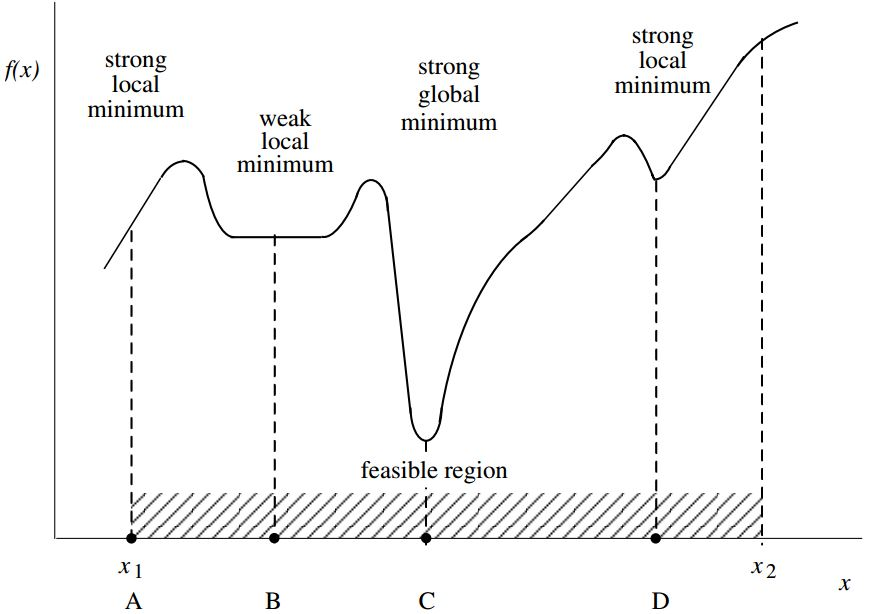
\includegraphics[width=\linewidth]{Images/min.jpg}
	\caption{Minimization points plotted}
\end{figure}
$\tilde{x}=x+\delta \quad \delta =\tilde{x}-x$ $\hat{f}(\tilde{x})=f(x)+g(x)(\tilde{x}-x)^T+0.5(\tilde{x}-x)^T H(x)(\tilde{x}-x)^T$
The gradient $g(x)$ and the Hessian $H(x)$ must satisfy certain conditions at a
local minimizer $x^*$.  \newline
1. Conditions which are satisfied at a local minimizer $x^*$.  \newline
2. Conditions which guarantee that $x^*$ is a local minimizer. 

\textbf{Definition 2.1} A point $x^* \in R,$ where R is the feasible region, is said to be a
weak local minimizer of f(x) if there exists a distance $\epsilon > 0$ such that
$f(x) \geq f(x^*)$ (2.5)
if
$x \in R$ and 
$||x-x^*|| < \epsilon$ \newline

\textbf{Definition 2.2} 
A point $x^* \in R $ is said to be a weak global minimizer of f(x) if
$f(x) \geq f(x^*)$ (2.6)
for all $x \in R.$  \newline
\textbf{Definition 2.3} 

If Eq. (2.5) in Def. 2.1 or Eq. (2.6) in Def. 2.2 is replaced by
$f(x) > f(x^*)$ (2.7)
$x^*$ is said to be a strong local (or global) minimizer. d

\textbf{Definition 2.4} Let $\delta = \alpha \mathbf{d}$ be a change in x where $\alpha$ is a positive constant and d is a direction vector. If R is the feasible region and a constant $\hat{\alpha} > 0$ exists such that
$x + \alpha d \in R$ for all $\alpha$ in the range $0 \leq \alpha \leq \hat{\alpha}$ , then d is said to be a feasible direction at
point x. \newline 

\textbf{Definition 2.5} \newline
(a) Let $d$ be an arbitrary direction vector at point $x$. The quadratic form
$d^TH(x)d$ is said to be \textit{positive definite, positive semidefinite, negative
	semidefinite, negative definite} if $d^TH(x)d > 0, \geq 0, \leq 0, < 0,$ respectively, for all $d \neq 0$ at $x$. If $d^TH(x)d$ can assume positive as well
as negative values, it is said to be indefinite. \newline
(b) If $d^TH(x)d$ is positive definite, positive semidefinite, etc., then matrix
$H(x)$ is said to be positive definite, positive semidefinite, etc. \newline

The objective function must satisfy two sets of conditions in order to have
a minimum, namely, first- and second-order conditions.  \newline
\textbf{First-order necessary conditions for a minimum} \newline %Theorem 2.2
(a) If $f(x) \in C^1$ and $x^*$ is a local minimizer, then
$g(x^*)^Td \geq 0$ for every feasible direction $d$ at $x^*$. \newline
(b) If $x^*$ is located in the interior of $\mathcal{R}$ then
$g(x^*) = 0$ \newline \newline 
\textbf{Second-order necessary conditions for a minimum} \newline
%Theorem 2.2
(a) If $f(x) \in C_2$ and $x^*$ is a local minimizer, then for every feasible direction
d at $x^*$. \hfill \break
\indent     $(i) \ g(x^*)Td \geq 0$ \newline
\indent    $(ii)$ If $g(x^*)^Td = 0$, then $d^TH(x^*)d \geq 0$ \newline
(b) If $x^*$ is a local minimizer in the interior of R, then \newline
\indent $ (i)$ $g(x^*) = 0$ \newline
\indent $ (ii)$ $d^TH(x^*)d \geq 0$ for all $d \neq 0$ 

\textbf{Second-order sufficient conditions for a minimum} \newline %Theorem 2.5
If $f(x) \in C_2$
and $x^*$ is located in the interior of $\mathcal{R}$, then the conditions
(a) $g(x^*) = 0$
(b) $H(x^*)$ is positive definite
are sufficient for $x^*$ to be a strong local minimizer. \newline

\textbf{Definition 2.6} \newline
A point $\bar{x} \in \mathcal{R},$ where $\mathcal{R}$ is the feasible region, is said to be a saddle point if \newline
(a) $g(\bar{x}) = 0$ \newline
(b) point $\bar{x}$ is neither a maximizer nor a minimizer. \hfill \break \newline
Stationary points can be located and classified as follows: \newline
1. Find the points $x_i$ at which $g(x_i) = 0$. \newline
2. Obtain the Hessian $H(x_i)$. \newline
3. Determine the character of $H(x_i)$ for each point $x_i$. \newline
If $H(x_i)$ is positive (or negative) definite, $x_i$ is a minimizer (or maximizer);
if $H(x_i)$ is indefinite, $x_i$ is a saddle point. 

\textbf{Techniques to compute Hessian P.D. , N.D. } \newline
Eigenvalues: det $ (\lambda I -A) = 0$ Multiplying all eigenvalues is equal to the determinant. \newline
The leading principal minors of a matrix A or its negative $-A$ can be used to
establish whether the matrix is positive or negative definite whereas the principal
minors of A or $-A$ can be used to establish whether the matrix is positive or
negative semidefinite. \newline 

\textbf{Theorem 2.9 Properties of matrices} \newline 
(a) If \textbf{H} is positive semidefinite or positive definite, then
det $\mathbf{H} \geq 0  \ \text{or} > 0$ \newline 
(b) \textbf{H} is positive definite if and only if all its leading principal minors are
positive, i.e., det $\mathbf{H_i} > 0$ for $ i = 1, 2, \cdots , n.$ \newline 
(c) \textbf{H} is positive semidefinite if and only if all its principal minors are nonnegative, i.e., det $(H_i^{(l)}) \geq 0$ for all possible selections of $\{l_1, l_2, \cdots , l_i \}$
for $i = 1, 2, \cdots, n$. \newline 
(d) \textbf{H} is negative definite if and only if all the leading principal minors of
$-\mathbf{H}$ are positive, i.e., $det ( -H_i) > 0$ for $i = 1, 2, \cdots, n$. \newline 
(e) \textbf{H} is negative semidefinite if and only if all the principal minors of -$\mathbf{H}$
are nonnegative, i.e., det $(-H_i^{(l)}) \geq 0$ for all possible selections of
$\{l_1, l_2, \cdots , l_i \}$ for $i = 1, 2, \cdots , n$. \newline 
(f) \textbf{H} is indefinite if neither (c) nor (e) holds. 

\textbf{Definition 2.7} \newline
A set $\mathcal{R}_c
\subset E_n $ is said to be convex if for every pair of points $x_1, x_2 \subset R_c$
and for every real number $\alpha$ in the range $0 < \alpha < 1$, the point
$x = \alpha x_1 + (1 - \alpha)x_2$
is located in $\mathcal{R}_c
$, i.e., $x \in \mathcal{R}_c$. \newline 

\textbf{Definition 2.8} \newline
(a) A function $f(x)$ defined over a convex set $\mathcal{R}_c$  is said to be convex if for
every pair of points $x_1, x_2 \in \mathcal{R}_c $ and every real number $\alpha$ in the range $0 < \alpha < 1$, the inequality
$f[\alpha x_1 + (1 - \alpha)x_2] \leq \alpha f(x_1) + (1 - \alpha)f(x_2)$ 
holds. If $x_1 \neq x_2$ and
$f[\alpha x_1 + (1 - \alpha)x_2] < \alpha f(x_1) + (1 - \alpha)f(x_2)$
then f(x) is said to be strictly convex. \newline
(b) If $\phi(x)$ is defined over a convex set $\mathcal{R}_c$ and f(x) = -$\phi(x)$ is convex, then $\phi(x)$ is said to be concave. If f(x) is strictly convex, $\phi(x)$ is strictly concave. \newline

\textbf{Property of convex functions relating to the Hessian} A function $f(x) \in C^2$is convex over a convex set 
$\mathcal{R}_c$ if and only if the Hessian H(x) of
f(x) is positive semidefinite for $x \in \mathcal{R}_c.$  \newline 

\textbf{Theorem 2.15 Relation between local and global minimizers in convex functions} \newline 
If $f(x)$ is a convex function defined on a convex set $\mathcal{R}_c$, then  \newline 
(a) the set of points $S_c$ where $f(x)$ is minimum is convex;  \newline 
(b) any local minimizer of $f(x)$ is a global minimizer. 

\section{Ch. 4}
\textbf{Dichotomous Search} \newline
Two function evaluations per iteration. \newline
A \textbf{unimodal function} on an interval has exactly
one point where a maximum or minimum
occurs in the interval. \newline 
Consider a unimodal function which is known to have a minimum in the interval $[x_L, \ x_U]$. This interval is said to be the range of uncertainty. \newline 
In this method, f(x) is evaluated at two points $x_a =
x_1 - \epsilon/2$ and $x_b = x_1 +\epsilon/2$ where $\epsilon$ is a small positive number. Then depending
on whether $f(x_a) < f(x_b)$ or $f(x_a) > f(x_b)$, range $x_L$ to $x_1 + \epsilon/2$ or $x_1 - \epsilon/2$
to $x_U$ can be selected and if $f(x_a) = f(x_b)$ either will do fine. If we assume
that $x_1 - x_L = x_U - x_1$, i.e., $x_1 = (x_L + x_U)/2$, the region of uncertainty
is immediately reduced by half. The same procedure can be repeated for the
reduced range, that is, f(x) can be evaluated at $x_2 - \epsilon/2$ and $x2 + \epsilon/2$ where $x_2$ is located at the center of the reduced range, and so on. \newline \newline 
%\begin{Figure}
%	\centering
%	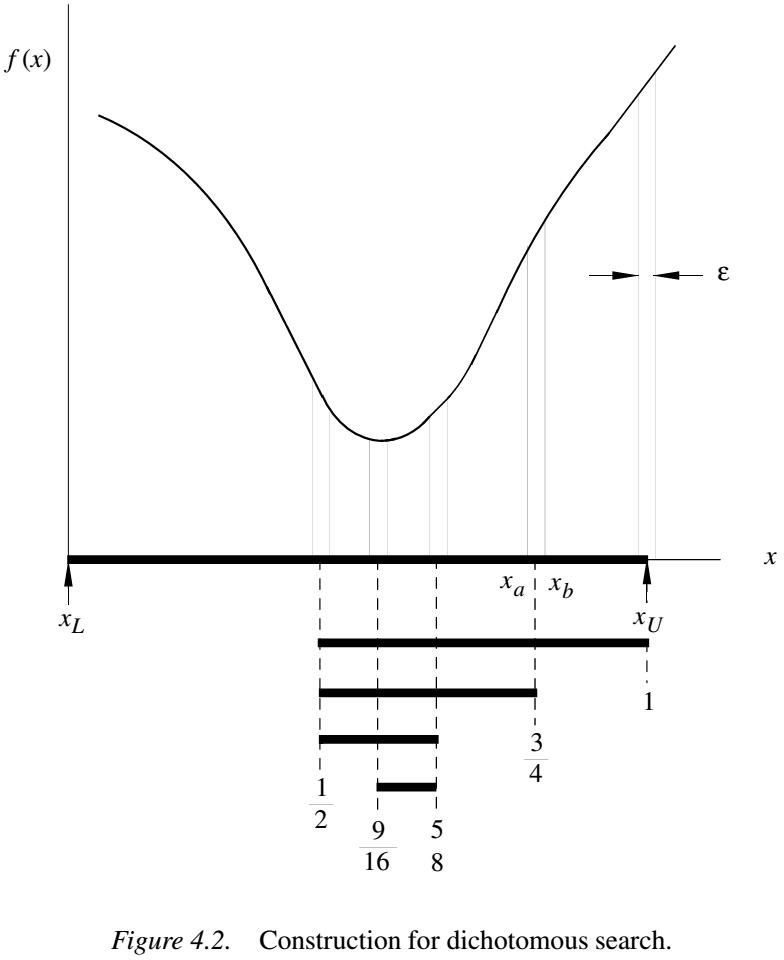
\includegraphics[width=\linewidth]{disearch}
%\end{Figure}
\textbf{Algorithm 4.1 Fibonacci} \newline
Computing n =$I_n=\frac{I_1}{F_n}$, function evaluations = n-1 \newline
\textbf{Step 1} \newline
Input $x_{L,1}, x_{U,1}$, and n. \newline
\textbf{Step 2} \newline
Compute $F_1, F_2, \cdots, F_n$ using Eq. (4.4). \newline
\textbf{Step 3} \newline
Assign $I_1 = x_{U,1} - x_{L,1}$ and compute
\begin{align*}
& I_2 = \frac{F_{n -1}}{F_n}I_1 (\text{see Eq. (4.6)})\\
& x_{a,1} = x_{U,1} - I_2, \quad x_{b,1} = x_{L,1} + I_2\\ 
& f_{a,1} = f(x_{a,1}), \quad f_{b,1} = f(x_{b,1})
\end{align*}
Set k = 1. \newline
\textbf{Step 4} \newline
Compute $I_{k+2}$ using Eq. (4.6).
If $f_{a,k} \geq f_{b,k}$, then update Eqs. (4.7) to (4.12) using
\begin{align*}
& x_{L,k+1}=x_{a,k} \\
& x_{U,k+1}=x_{U,k} \\
& x_{a,k+1}=x_{b,k} \\
& x_{b,k+1}=x_{L,k+1}+I_{k+1} \\
& f_{a,k+1}=f_{b,k} \\
& f_{b,k+1}=f(x_{b,k+1})
\end{align*}
using  Otherwise, if $f_{a,k} < f_{b,k}$, update
information using Eqs. (4.13) to (4.18) using \newline
\begin{align*}
& x_{L,k+1}=x_{L,k} \\
& x_{U,k+1}=x_{b,k} \\
& x_{a,k+1}=x_{U,k+1}-I_{k+2} \\
& x_{b,k+1}=x_{a,k} \\
& f_{a,k+1}=f(x_{a,k+1}) \\
& f_{b,k+1}=f_{a,k}
\end{align*}

\textbf{Step 5} \newline
If $k = n - 2$ or $x_{a,k+1} > x_{b,k+1}$, output $x^* = x_{a,k+1}$ and $f^* = f(x^*)$,
and stop. Otherwise, set $k = k + 1$ and repeat from Step 4.
The condition $x_{a,k+1} > x_{b,k+1}$ implies that $x_{a,k+1} \approx x_{b,k+1}$ within the precision of the computer used, as was stated earlier, or that there is an error in the algorithm. It is thus used as an alternative stopping criterion. \newline

\textbf{Algorithm 4.2 Golden-section search} \newline
(function evaluations = k+1) and Golden Ratio: $K=\cfrac{1+\sqrt{5}}{2}$
$\Lambda_{GS} = I_n = \frac{I_1}
{K_{n-1}}$ \quad $\Lambda_{F} = I_n = \frac{I_1}
{F_n} \approx \frac{\sqrt{5}}
{K^{n+1}}I_1$
$\frac{I_k}{I_{k+1}}=\frac{I_{k+1}}{I_{k+2}}
= \frac{I_{k+2}}{I_{k+3}}
= \cdots = K$ \newline
\textbf{Step 1} \newline
Input $x_{L,1}, x_{U,1},$ and $\epsilon$. \newline
\textbf{Step 2} \newline
Assign $I_1 = x_{U,1} - x_{L,1}, K = 1.618034$ and compute
\begin{align*}
&I_2 = I_1/K \\
&x_{a,1} = x_{U,1} - I_2, \quad x_{b,1} = x_{L,1} + I_2 \\
&f_{a,1} = f(x_{a,1}), \quad f_{b,1} = f(x_{b,1}) 
\end{align*}
Set $k = 1$. \newline
\textbf{Step 3} \newline
Compute $I_{k+2} = I_{k+1}/K$ \newline
If $f_{a,k} \geq f_{b,k}$, then update $x_{L,k+1}, x_{U,k+1}$, $x_{a,k+1}$, $x_{b,k+1}$, $f_{a,k+1}$,
and $f_{b,k+1}$ as  
\begin{align*}
& x_{L,k+1}=x_{a,k} \\
& x_{U,k+1}=x_{U,k} \\
& x_{a,k+1}=x_{b,k} \\
& x_{b,k+1}=x_{L,k+1}+I_{k+1} \\
& f_{a,k+1}=f_{b,k} \\
& f_{b,k+1}=f(x_{b,k+1})
\end{align*}
Or use using Eqs. (4.7) to (4.12). 
Otherwise if $f_{a,k} < f_{b,k}$, then update $x_{L,k+1}, x_{U,k+1}$, $x_{a,k+1}$, $x_{b,k+1}$, $f_{a,k+1}$, and $f_{b,k+1}$ as
\begin{align*}
& x_{L,k+1}=x_{L,k} \\
& x_{U,k+1}=x_{b,k} \\
& x_{a,k+1}=x_{U,k+1}-I_{k+2} \\
& x_{b,k+1}=x_{a,k} \\
& f_{a,k+1}=f(x_{a,k+1}) \\
& f_{b,k+1}=f_{a,k}
\end{align*}
Otherwise, if $f_{a,k} < f_{b,k}$, update
information using Eqs. (4.13) to (4.18). \newline
\textbf{Step 4} \newline
If $I_k < \epsilon$ or $x_{a,k+1} > x_{b,k+1}$, then do: \newline
If $f_{a,k+1} > f_{b,k+1}$, compute
$x^* = 0.5(x_{b,k+1} + x_{U,k+1})$ \newline
If $f_{a,k+1} = f_{b,k+1}$, compute
$x^* = 0.5(x_{a,k+1} + x_{b,k+1})$ \newline
If $f_{a,k+1} < f_{b,k+1}$, compute
$x^* = 0.5(x_{L,k+1} + x_{a,k+1})$
Compute $f^* = f(x^*).$ \newline
Output $x^*$ and $f^*$, and stop. \newline
\textbf{Step 5} \newline
Set $k = k + 1$ and repeat from Step 3. \newline \newline 
\textbf{Equations 4.4, 4.6, (4.7-4.12) and (4.13-4.18) } \newline
$F_k = F_{k-1} + F_{k-2} \quad$ for $k \geq 2$ (4.4) \newline
$I_{k+2} = \frac{F_{n-k-1}}{F_{n-k}}I_{k+1} (4.6)$

If $f_{a,k} > f_{b,k}$, then $x^*$ is in interval $[x_{a,k}, x_{U,k}]$ and so the new bounds of $x^* \rightarrow$  %\newline 
$x_{L,k+1} = x_{a,k} (4.7) \quad x_{U,k+1} = x_{U,k} (4.8)$ 
Similarly, the two interior points of the new interval, namely, $x_{a,k+1}$ and $x_{b,k+1}$
will be $x_{b,k}$ and $x_{L,k+1} + I_{k+2}$, respectively. We can thus assign
$x_{a,k+1} = x_{b,k}$ (4.9) $x_{b,k+1} = x_{L,k+1} + I_{k+2}$ (4.10)
as illustrated in Fig. 4.5. \newline
The value $f_{b,k}$ is retained as the value of f(x) at
$x_{a,k+1}$, and the value of f(x) at $x_{b,k+1}$ is calculated, i.e.,
$f_{a,k+1} = f_{b,k}$ (4.11)
$f_{b,k+1} = f(x_{b,k+1})$ (4.12) \newline
%\begin{Figure}
%	\centering
%	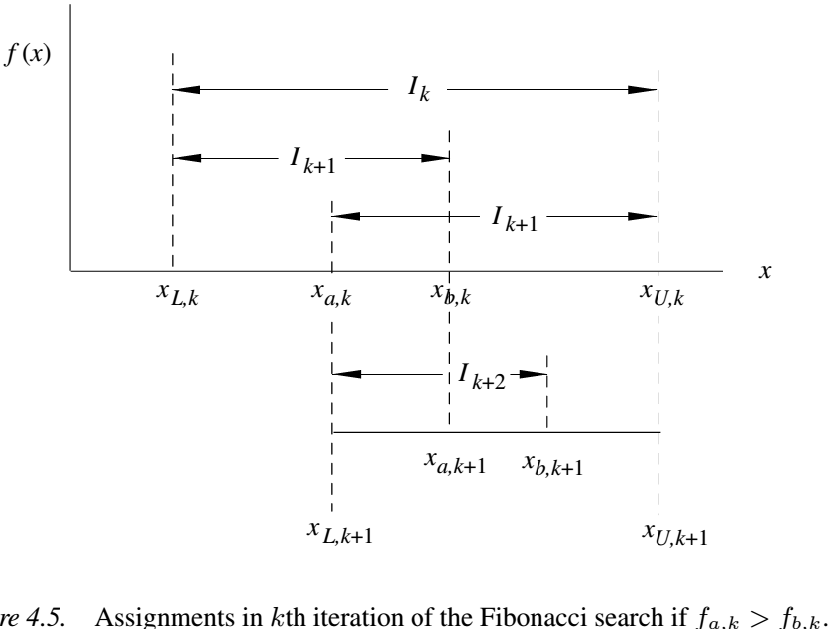
\includegraphics[width=\linewidth]{fibfirst}
%\end{Figure}
On the other hand, if $f_{a,k} < f_{b,k}$, then $x^*$ is in interval $[x_{L,k}, x_{b,k}]$. In this
case, we assign
$x_{L,k+1} = x_{L,k}$ (4.13)
$x_{U,k+1} = x_{b,k}$ (4.14)
$x_{a,k+1} = x_{U,k+1} - I_{k+2}$ (4.15)
$x_{b,k+1} = x_{a,k}$ (4.16)
$f_{b,k+1} = f_{a,k}$ (4.17)
and calculate
$f_{a,k+1} = f(x_{a,k+1})$ (4.18) \newline  \newline
%\begin{Figure}
%	\centering
%	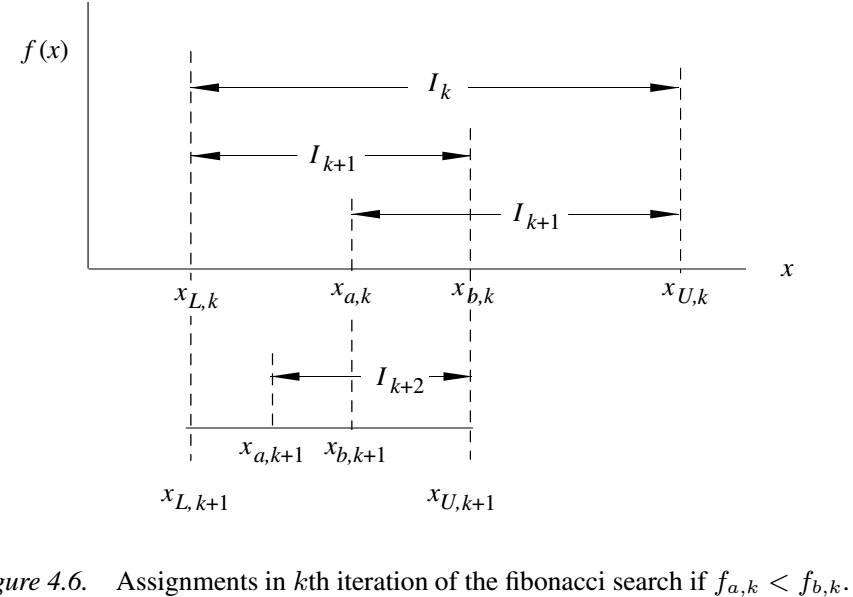
\includegraphics[width=\linewidth]{fibsecond}
%\end{Figure}
%\begin{Figure}
%	\centering
%	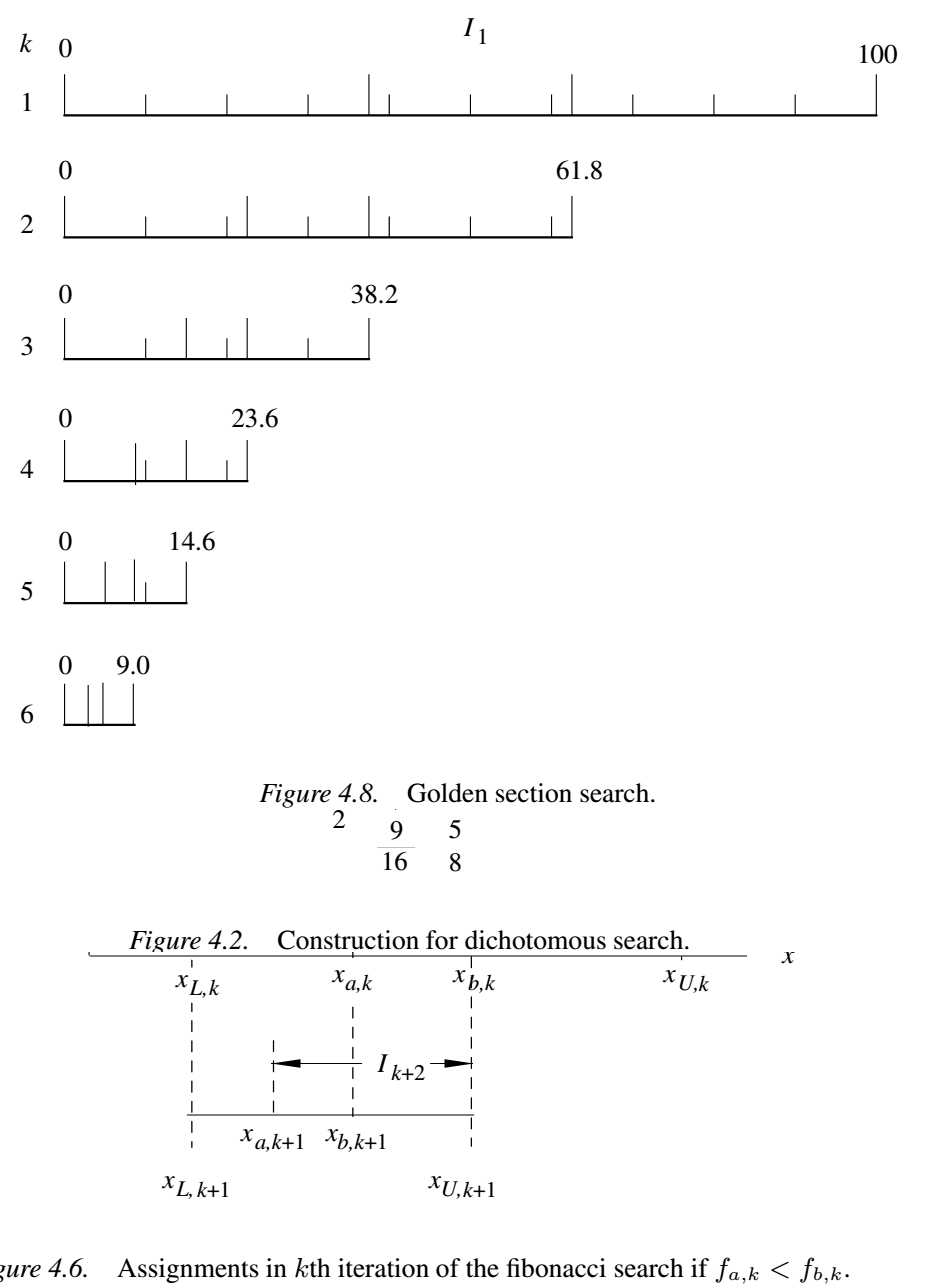
\includegraphics[width=\linewidth]{golden}
%\end{Figure}
%\begin{Figure}
%	\centering
%	\includegraphics[width=\linewidth]{fib}
%\end{Figure}
%%%%%%%%%%%%%%%%%%%%%%%%%%%%%%%
%% Unlikely to be tested %%
%% INCLUDE FOR FINAL %%
%%%%%%%%%%%%%%%%%%%%%%%%%%%%%%%
\textbf{Algorithm 4.6 Inexact line search}  \newline
\textbf{Step 1:} \newline
Input $x_k$, $d_k$, and compute $g_k$. \newline
Initialize algorithm parameters $\rho, \sigma, \tau$, and $\chi$. \newline
Set $\alpha_L = 0$ and $\alpha_U = 10^{99}$. \newline
\textbf{Step 2:} \newline
Compute $f_L = f(x_k + \alpha_L dk)$. \newline
Compute $f_L^\prime = g(x_k + \alpha_L dk)^Tdk$. \newline
\textbf{Step 3:} \newline
Estimate $\alpha_0$. \newline
\textbf{Step 4:} \newline
Compute $f_0 = f(x_k + \alpha_0dk)$. \newline
\textbf{Step 5 (Interpolation)} \newline
If $f_0 > f_L + \rho(\alpha_0 - \alpha_L)f_L^\prime$ , then do: \newline
a. If $\alpha_0 < \alpha_U$, then set $\alpha_U = \alpha_0$.\newline
b. Compute $\breve{\alpha}_0$ using the interpolation formula Eq. (4.57). %\newline
\[
\breve{\alpha}_0 =\alpha_L + \frac{(\alpha_0-\alpha_L)^2f_L^\prime}{2[f_L-f_0+(\alpha_0-\alpha_L)f_L^\prime]}
\]
c. If $\breve{\alpha}_0 < \alpha_L + \tau(\alpha_U - \alpha_L)$ then set $\breve{\alpha}_0 = \alpha_L + \tau(\alpha_U - \alpha_L)$. \newline
d. If $\breve{\alpha}_0 > \alpha_U - \tau(\alpha_U - \alpha_L)$ then set $\breve{\alpha}_0  = \alpha_U - \tau(\alpha_U - \alpha_L)$. \newline
e. Set $\alpha_0 = \breve{\alpha}_0$ and go to Step 4. \newline
\textbf{Step 6} \newline
Compute $f_0^\prime = g(x_k + \alpha_0dk)^Tdk$. \newline
\textbf{Step 7 (Extrapolation)} \newline
If $f_0^\prime < \alpha f_L^\prime$ , then do: \newline
a. Compute $\nabla \alpha_0 = (\alpha_0 - \alpha_L)f_0^\prime /(f_L^\prime - f_0^\prime)$ (see Eq. (4.58)).
\[
\breve{\alpha}_0 = \alpha_0 + (\alpha_0 - \alpha_L)f_0^\prime
(f_L^\prime - f_0^\prime) \quad (Eq. (4.58))
\]
b. If $\nabla \alpha_0 < \tau(\alpha_0 - \alpha_L)$, then set $\nabla \alpha_0 = \tau(\alpha_0 - \alpha_L)$. \newline
c. If $\nabla \alpha_0 > \chi(\alpha_0 - \alpha_L)$, then set $\nabla \alpha_0 = \chi(\alpha_0 - \alpha_L)$. \newline
d. Compute $\breve{\alpha}_0 = \alpha_0 + \nabla \alpha_0$. \newline
e. Set $ \alpha_L =  \alpha_0, \alpha_0 = \breve{\alpha}_0, f_L = f_0, f_L^\prime = f_0^\prime$, and go to Step 4. \newline
\textbf{Step 8} \newline
Output $\alpha_0$ and $f_0 = f(x_k + \alpha_0dk)$, and stop.


\section{Ch. 5}
Standard form: $f(x)=\frac{1}{2}x^T H x + x^T g(x) + C$ \newline 
Rate of Convergence $\beta = (1-r^2)/(1+r^2)$, where r is the smallest eigenvalue divided by the biggest eigenvalue. \newline
\begin{align*}
& H^{-1}=\begin{bmatrix}
a & c \\
c & b 
\end{bmatrix}^{-1}
=
\frac{1}{ab-c^2}
\begin{bmatrix}
b & -c \\
-c & a
\end{bmatrix} \quad ab-c^2 \neq 0
\end{align*}
$[f(x_k)-f(x^*)]\leq \left(\frac{1-r}{1+r}\right)^2[f(x_k)-f(x^*)]$ \newline
\textbf{Algorithm 5.1 Steepest-descent algorithm} \newline
\textbf{Step 1}  \newline
Input $x_0$ and initialize the tolerance $\epsilon$. \newline
Set $k = 0$. \newline
\textbf{Step 2} \newline
Calculate gradient $g_k$ and set $d_k=-g_k$. \newline
\textbf{Step 3} \newline
Find $\alpha_k$, the value of $\alpha$ that minimizes $f(x_k + \alpha d_k)$, using a line search (Algorithm Inexact Line Search. 4.6). \newline
\textbf{Step 4} \newline
Set $x_{k+1} = x_k + \alpha_k d_k$ and calculate $f_{k+1} = f(x_{k+1})$. \newline
\textbf{Step 5}  \newline
If $||\alpha_k d_k|| < \epsilon$, then do: \newline
Output $x^* = x_{k+1}$ and $f(x^*) = f_{k+1}$, and stop. \newline
Otherwise, set $k = k + 1$ and repeat from Step 2. \newline 

\textbf{Algorithm 5.3 Basic Newton algorithm} \newline
\textbf{Step 1} \newline
Input $x_0$ and initialize the tolerance $\epsilon$ \newline
Set $k = 0$. \newline
\textbf{Step 2} \newline
Compute $g_k$ and $H_k$. \newline
If $H_k$ is not positive definite, force it to become positive definite. \newline
\textbf{Step 3} \newline
Compute $H_k^{-1}$ and $d_k=-H_k^{-1}g_k$ \newline
\textbf{Step 4} \newline
Find $\alpha_k$ , the value of $\alpha$ that minimizes $f(x+\alpha d_k)$, using a line search. \newline
\textbf{Step 5} \newline
Set $x_{k+1}=x_k+\alpha_k d_k$ \newline
Compute $f_{k+1}=f(x_{k+1})$. \newline
\textbf{Step 6} \newline
If $||\alpha_k d_k|| < \epsilon$, then do:  \newline
Output $x^*=x_{k+1}$ and $f(x^*)=f(x_{k+1})$, and stop \newline
Otherwise, set $k = k + 1$ and repeat from Step 2. \newline
\textbf{Algorithm 5.5 Gauss --- Newton Algorithm} \newline
$f=\begin{bmatrix}
f_1(x)  & f_2(x) & \cdots f_m(x)
\end{bmatrix}^T$, J = Jacobian \newline
$F(x)=\sum_{p=1}^{m}f_p(x)^2=f^Tf$ \newline
$J=\begin{bmatrix}
\frac{ \partial f_1}{\partial  x_1} & \frac{ \partial  f_1}{ \partial  x_2} & \cdots & \frac{\partial  f_1}{\partial  x_n} \\
\frac{\partial  f_2}{\partial x_1} & \frac{\partial  f_2}{\partial  x_2} & \cdots & \frac{\partial  f_2}{\partial x_n} \\
\vdots & \vdots & \ddots & \vdots \\
\frac{\partial f_m}{\partial  x_1}& \frac{\partial f_m}{\partial  x_2}& \cdots & \frac{\partial f_m}{\partial x_n}
\end{bmatrix}$ \newline
\textbf{Step 1} \newline
Input $x_0$ and initialize the tolerance $\epsilon$.  \newline
Set $k = 0$. \newline
\textbf{Step 2} \newline
Compute $f_{pk} = f_p(x_k)$ for $p = 1, 2, \cdots, m$ and $F_k$.
\newline
\textbf{Step 3}  \newline
Compute $J_k, g_k = 2J^T_k f_k$, and $H_k = 2J^T_k J_k$. \newline
\textbf{Step 4}  \newline
$d_k=-H_k^{-1}g_k$ \newline
\textbf{Step 5} \newline
Find $\alpha_k$, the value of $\alpha$ that minimizes $f(x_k + \alpha d_k)$. \newline
\textbf{Step 6} \newline
Set $x_{k+1} = x_k + \alpha_kd_k$. \newline
Compute $f_{p,k+1}$ for $p = 1, 2,\cdots, m$ and $F_{k+1}$. \newline
\textbf{Step 7} \newline
If $|F_{k+1}-F_k | < \epsilon$, then do: \newline
Output $x^*= x_{k+1}$, $f_{p,k+1}(x^*)$ for $p = 1, 2,\cdots, m$, and $F_{k+1}$. \newline
Stop. \newline
Otherwise, set $k = k + 1$ and repeat from Step 3.


\section{Ch. 7}
\textbf{Problems with Rank-one Method}
\begin{enumerate}
	\item positive definite $S_k$ may not yield positive definite $S_{k+1}$
	\item denominator in correction formula may approach zero 
\end{enumerate}  
THE DFP and BFGS are implementing of the basic algorithms Quasi Newton (7.2) with changes to the updating function. $d_k=-S_kg_k$ and $f(x_k + \alpha d_k)$  $\rightarrow$  $\alpha_k=\frac{g_k^TS_kg_k} 
{g_k^TS_kHS_kg_k}$ \newline
Convergence equation: $\beta = \left(\frac{1-r}{1+r}\right)^2$ $f(x_{k+1})-f(x^*) \leq \left(\frac{1-r}{1+r}\right)^2[f(x_k)-f(x^*)]$ \newline
\textbf{BFGS and then DFP properties} \newline
For convex quadratic functions (BFGS)
\begin{enumerate}
	\item[---] $Sk+1$ becomes identical to $H^{-1}$ for $k = n-1$.
	\item[---] Directions $\delta_0,\delta_1,\cdots,\delta_{n-1}$ form a conjugate set. 
	\item[---] $S_{k+1}$ is positive definite if $S_k$ is positive definite.
	\item[---] $\delta^T_k \gamma_k = \delta^T_k g_{k+1}-\delta_T^k g_k > 0$ applies. \newline
\end{enumerate}  
\textbf{For DFP (from textbook)} 
\begin{enumerate}
	\item If $S_k$ is PD, then 
	the matrix $S_{k+1}$ generated by DFP is also PD.
	\item Directions $\delta_0,\delta_1,\cdots,\delta_{n-1}$ form a conjugate set. \newline
\end{enumerate} 
\textbf{Algorithm 7.2 adjusted for DFP/BFGS} \newline
\textbf{Step 1} \newline
Input $x_0$  and initialize the tolerance $\epsilon$. \newline
Set $k = 0$ and $S_0 = I_n$. \newline
Compute $g_0$. \newline
\textbf{Step 2} \newline
Set $d_k=-S_kg_k$ \newline
Find $\alpha_k$, the value of $\alpha$ that minimizes $f(x_k+\alpha d_k)$, using a line search \newline
Set $\delta_k=\alpha_k d_k$ and $x_{k+1}=x_k+\delta_k$ \newline
\textbf{Step 3} \newline
If $||\delta_k|| < \epsilon$, output $x^* = x_{k+1}$ and $f(x^*) = f(x_{k+1})$, and stop \\
\textbf{Step 4} \newline
Compute $g_{k+1}$ and set $\gamma_k=g_{k+1}-g_k$ \newline
Compute $S_{k+1}$ using appropriate formula.
\begin{align*}
&\text{Basic/ Rank One:} \quad S_{k+1}=S_k+\frac{(\delta_k-S_k \gamma_k)(\delta_k-S_k \gamma_k)^T}{\gamma_k^T(\delta_k-S_k\gamma_k)}\\
&\text{DFP:}\quad S_{k+1}=S_k+\frac{\delta_k \delta_k^T}{\delta_k^T \gamma_k}-\frac{S_k\gamma_k\gamma_k^TS_k}{\gamma_k^TS_k\gamma_k}\\
&\text{BFGS:} \quad S_{k+1}=S_k+\left(1+\frac{\gamma_k^TS_k\gamma_k}{\gamma_k^T\delta_k}\right)\frac{\delta_k\delta_k^T}{\gamma_k^T\delta_k}-\frac{(\delta_k\gamma_k^TS_k+S_k\gamma_k\delta_k^T)}{\gamma_k^T\delta_k}
\end{align*}
Set $k=k+1$ and repeat from Step 2. \newline
\begin{itemize}
	\item[---] remember that $\left(1+\frac{\gamma_k^TS_k\gamma_k}{\gamma_k^T\delta_k}\right)$ is a single number
	\item[---] $\delta_k\delta_k^T$ is a matrix.
	\item[---] Focus on minimization, $\max[f(x)] =-\min[-f(x)]$
	\item[---] Hessian is positive semidefinite for concave functions.
\end{itemize}
\end{multicols}
\chapter{ELEC 360 CheatSheet}
Some keywords used can be found in the glossary section including:
\begin{itemize}
	\item  \gls{partFrac}, \gls{openLoop}, \gls{SISO}, \gls{MIMO}, and \gls{LTI}
	\item  \gls{conSys}, \gls{closedLoop}, \gls{DC Motors}, and \gls{Op Amps}
\end{itemize}

\begin{multicols}{3}

%\includegraphics[width=1.77165in,height=0.95669in]{media/image1.png}

\section{LAPLACE TRANSFORMS}

Final Value Theorem

In Control Engineering, the Final Value Theorem is used most frequently to determine the steady-state value of a system. The real part of the poles of the function must be < 0.
\begin{align}
& \lim\limits_{t \rightarrow \infty} x(t) = \lim\limits_{t \rightarrow 0} sX(s)
\end{align}
%\includegraphics[width=1.77165in,height=0.92126in]{media/image2.png}

%\includegraphics[width=1.77165in,height=1.14961in]{media/image3.png}

Initial Value Theorem

\begin{align}
& \lim\limits_{t \rightarrow 0} x(t) = \lim\limits_{t \rightarrow \infty} sX(s)
\end{align}
%\includegraphics[width=1.77165in,height=0.90551in]{media/image4.png}

%\includegraphics[width=1.77165in,height=0.77953in]{media/image5.png}

\section{SOLUTION OF LINEAR DIFFERENTIAL EQUATION}

\[A\ddot{y} + B\dot{y} + Cy = u\left( t \right)\]

\[\text{with initial conditions }\dot{y}\left( 0 \right)\ and \ y(0)\]

\[\text{is solved by constructing the equation}\]

%\[A\left\lbrack s^{2}Y\left( s \right) - sy\left( 0 \right) - \dot{y}\left( 0 \right) \right\rbrack + B\left\lbrack \text{sY}\left( s \right) - y\left( 0 \right) \right\rbrack + CY(s)\]

\begin{align*}
 &A\left\lbrack s^{2}Y\left( s \right) - sy\left( 0 \right) - \dot{y}\left( 0 \right) \right\rbrack + B\left\lbrack \text{sY}\left( s \right) - y\left( 0 \right) \right\rbrack \\
 & + CY(s)
\end{align*}
\[that\ is\ to\ say:\]

\[\mathcal{L}\left\{ \ddot{y} \right\} = s^{2}Y\left( s \right) - sy\left( 0 \right) - \dot{y}(0)\]

\[\text{and}\]

\[\mathcal{L}\left\{ \dot{y} \right\} = sY\left( s \right) - y\left( 0 \right)\]

\section{STATESPACE REPRESENTATIONS}

To generate from a differential equation:

Use the \textbf{closed loop transfer function}

\[\frac{Y\left( s \right)}{U\left( s \right)} = \frac{s + A}{s^{3} + \text{Bs}^{2} + s + A}\]

Separate and take the inverse Laplace transform

\begin{align*} &s^{3}Y\left( s \right) + \text{Bs}^{2}Y\left( s \right) + sY\left( s \right) + AY\left( s \right) \\
 &= sU\left( s \right) + AU\left( s \right)
 \end{align*}

\[= \dddot{y} + B\ddot{y} + \dot{y} + Ay = \dot{u} + Au\]

Then define state variables:

\(x_{1} = y\) \(\dot{x_{1}} = \dot{y} = x_{2}\)

\(x_{2} = \dot{y}\) \(\dot{x_{2}} = \ddot{y} = x_{3}\)

\(x_{3} = \ddot{y}\)
\(\dot{x_{3}} = \dddot{y} = \dot{u} + Au - B\ddot{y} - \dot{y} - Ay\)

Then construct the state space matrix

\[\begin{bmatrix}
\dot{x_{1}} \\
\dot{x_{2}} \\
\dot{x_{3}} \\
\end{bmatrix} = \begin{bmatrix}
0 & 1 & 0 \\
0 & 0 & 1 \\
 - A & - 1 & - B \\
\end{bmatrix}\begin{bmatrix}
x_{1} \\
x_{2} \\
x_{3} \\
\end{bmatrix} + \begin{bmatrix}
\beta_{1} \\
\beta_{2} \\
\beta_{3} \\
\end{bmatrix}u\]

and

\[y = \begin{bmatrix}
1 & 0 & 0 \\
\end{bmatrix}\begin{bmatrix}
x_{1} \\
x_{2} \\
x_{3} \\
\end{bmatrix} + \beta_{0}u\]

\(\beta\) values can be calculated as follows:

\[\beta_{0} = b_{0}\]

\[\beta_{1} = b_{1} - a_{1}\beta_{0}\]

\[\beta_{2} = b_{2} - a_{1}\beta_{1} - a_{2}\beta_{0}\]

\[\beta_{3} = b_{3} - a_{1}\beta_{2} - a_{2}\beta_{1} - a_{3}\beta_{0}\]

Where the values for \(a_{x}\text{\ and\ }b_{x}\)come from:

\[\dddot{y} + a_{1}\ddot{y} + a_{2}\dot{y} + a_{3}y = b_{0}\dddot{u} + b_{1}\ddot{u} + b_{2}\dot{u} + b_{3}u\]


\[\ddot{x}=(F-c\dot{x_{1}}-kx)/m\]
where
	x=position,$\dot{x}$=speed/velocity,$\ddot{x}$=acceleration
	c = damping constant,
	m = mass,
	F = force
	k = spring constant,

To perform inverse (find transfer function from statespace model)

\[G\left( s \right) = d + c{(sI - A)}^{- 1}b\]


where

\[\begin{bmatrix}
\dot{x_{1}} \\
\dot{x_{2}} \\
\dot{x_{3}} \\
\end{bmatrix} = \begin{bmatrix}
A_{11} & A_{12} & A_{13} \\
A_{21} & A_{22} & A_{23} \\
A_{31} & A_{32} & A_{33} \\
\end{bmatrix}\begin{bmatrix}
x_{1} \\
x_{2} \\
x_{3} \\
\end{bmatrix} + \begin{bmatrix}
b_{1} \\
b_{2} \\
b_{3} \\
\end{bmatrix}u\]

And

\[y = \begin{bmatrix}
c_{1} & c_{2} & c_{3} \\
\end{bmatrix}\begin{bmatrix}
x_{1} \\
x_{2} \\
x_{3} \\
\end{bmatrix} + \lbrack d\rbrack u\]

The inverse of a square 2x2 matrix is found by:

\[\begin{bmatrix}
a & b \\
c & d \\
\end{bmatrix}^{- 1} = \frac{1}{ad - bc}\begin{bmatrix}
d & - b \\
 - c & a \\
\end{bmatrix}\]

The inverse of a square 3x3 matrix is found by:
%\includegraphics[width=2.52147in,height=1.02367in]{media/image8.png}

For a 3×3 matrix
$$A=\begin{bmatrix}
	a_{11} & a_{12}  & a_{13} \\
	a_{21} & a_{22}  & a_{23}\\
	a_{31} & a_{32}  &  a_{33}
\end{bmatrix}$$	
the matrix inverse is:

$$A^{-1}= \frac{1}{|A|}\begin{bmatrix}
\begin{bmatrix} a_{22} & a_{23} \\ a_{32} & a_{33}\end{bmatrix} & \begin{bmatrix} a_{13} & a_{12} \\ a_{33} & a_{32}\end{bmatrix} & \begin{bmatrix} a_{12} & a_{13} \\ a_{22} & a_{23}\end{bmatrix} \\
\begin{bmatrix} a_{23} & a_{21} \\ a_{33} & a_{31}\end{bmatrix}& \begin{bmatrix} a_{11} & a_{13} \\ a_{31} & a_{33}\end{bmatrix} & \begin{bmatrix} a_{13} & a_{11} \\ a_{23} & a_{21}\end{bmatrix} \\
\begin{bmatrix} a_{21} & a_{22} \\ a_{31} & a_{32}\end{bmatrix} & \begin{bmatrix} a_{12} & a_{11} \\ a_{32} & a_{31}\end{bmatrix} & \begin{bmatrix} a_{11} & a_{12} \\ a_{21} & a_{22}\end{bmatrix}	
\end{bmatrix}$$
Solving a three order polynomial, without a fancy calculator
\begin{align*}
& x = \left[q + \left[ q^2 + (r-p^2)^3\right ]^{1/2} \right]^{1 /3} \\
& \left[q - \left[ q^2 + (r-p^2)^3\right ]^{1/2} \right]^{1 /3} + p
\end{align*}
Where 
\begin{align*}
& p = \frac{-b}{3a}, \ \ q =p^3 + \frac{bc-3ad}{3a^2}, \ \ r =\frac{c}{3a}
\end{align*}
\section{SECOND ORDER SYSTEMS}

\[G\left( s \right) = \frac{C(s)}{R(s)} = \frac{\omega_{n}^{2}}{s^{2} + 2\zeta\omega_{n}s + \omega_{n}^{2}}\]

\[K = \omega_{n}^{2};\ \ \ \ T = 2\zeta\omega_{n} = 2\sigma;\ \ \ \ \ \zeta = \frac{T}{2\sqrt{K}};\ \ \ \ \omega_{d} = \omega_{n}\sqrt{1 - \zeta^{2}}\]

\[\zeta = damping\ ratio; \sigma = real\ part\ of\ root;\]

\(\ \ \ \omega_{d} = damped\ natural\ frequency\)

\( omega_{n} = undamped\ natural\ frequency \)
%\includegraphics[width=1.96736in,height=1.37361in]{media/image9.png}

\[ Undamped:\ \zeta = 0;\] 
\[ Critically\ Damped: \zeta = 1 \] 
\[ Over\ Damped:\ \zeta > 1\]

Imaginary axis:

Frequency of oscillations

Real axis:

Decay time

\textbf{UNIT STEP RESPONSE OF A 2\textsuperscript{ND} ORDER UNDAMPED
SYSTEM}

$ t_{d}$ = delay time - to reach 50\% of $c\left( \infty \right) $\text{for the first time}.
$ t_{r}$ = rise time - time to reach 100 \% of $c\left( \infty \right)$ \text{for first time} . 
$ t_{p}$ = peak time - time to reach first peak. 
$ t_{s}$ = settling time - time to reach \& stay within 2\% or 5\% 
$ M_{p}$ = maximum overshoot. 
%\[{t_{d} = delay\ time - to\ reach\ 50\%\ of\ c\left( \infty \right)\text{for\ the\ first\ time}\backslash n}{t_{r} = rise\ time - time\ to\ reach\ 100\%\ of\ c\left( \infty \right)\text{for\ first\ time}\backslash n}{t_{p} = peak\ time - time\ to\ reach\ first\ peak\backslash n}{t_{s} = settling\ time - time\ to\ reach\ \&\ stay\ within\ 2\%\ or\ 5\%\backslash n}{M_{p} = maximum\ overshoot\ \left( \% \right)\backslash n}\]
\[{t_{r} = \frac{1}{\omega_{d}}\operatorname{}\left( - \frac{\omega_{d}}{\sigma} \right);\ \ \ \ t_{p} = \frac{\pi}{\omega_{d}}\backslash n}\]

\[{M_{p} = e^{- \frac{\zeta\omega_{n}\pi}{\omega_{d}}} = e^{- \frac{\eta \pi}{\sqrt{1 - \zeta^{2}}}} = e^{- \frac{\sigma \pi}{\omega_{d}}}}\]

\[t_{s} = \frac{4}{\sigma} = \frac{4}{\zeta\omega_{n}}\ \left( 2\%\ band \right)\]
\[t_{s} = \frac{3}{\sigma} = \frac{3}{\zeta\omega_{n}}\ \left( 5\%\ band \right)\]

Dominant poles are the ones closest to the imaginary axis

\section{ROUTH-HURWITZ STABILITY TEST}
\[a_0s^n + a_1s^{n-1}+ \cdots + a{n-1} s + a_n = 0\]
\[ \begin{array}{lllll}
\mbox{row n}   & a_0 & a_2 & a_4 & \cdots \\
\mbox{row n-1} & a_1 & a_3 & a_5 & \cdots \\
\mbox{row n-2} & b_1 & b_2 & b_3 & \cdots \\
\mbox{row n-3} & c_1 & c_2 & c_3 & \cdots \\
\cdots & \cdots & \cdots & \cdots & \cdots \\
\mbox{row 2} & * & * &  & \cdots \\
\mbox{row 1} & * &   &  & \cdots \\
\mbox{row 0} & * &   &  & \cdots \end{array} \]

\[ b_1=-\frac{det\left[\begin{array}{cc}a_0&a_2\\a_1&a_3\end{array}\right]}{a_1}
=\frac{a_1a_2-a_0a_3}{a_1} \]
\[ b_2=-\frac{det\left[\begin{array}{cc}a_0&a_4\\a_1&a_5\end{array}\right]}{a_1}
=\frac{a_1a_4-a_0a_5}{a_1} \]
\[ b_3=-\frac{det\left[\begin{array}{cc}a_0&a_6\\a_1&a_7\end{array}\right]}{a_1}
=\frac{a_1a_6-a_0a_7}{a_1} \]

\[ c_1=-\frac{det\left[\begin{array}{cc}a_1&a_3\\b_1&b_2\end{array}\right]}{b_1}
=\frac{b_1a_3-a_1b_2}{b_1} \]
\[ c_2=-\frac{det\left[\begin{array}{cc}a_1&a_5\\b_1&b_3\end{array}\right]}{b_1}
=\frac{b_1a_5-a_1b_3}{b_1} \]
\[ c_3=-\frac{det\left[\begin{array}{cc}a_1&a_7\\b_1&b_4\end{array}\right]}{b_1}
=\frac{b_1a_7-a_1b_4}{b_1} \]
\section{STEADY STATE ERROR ANALYSIS}

\[K_{p} = \operatorname{}{G\left( s \right)H(s)}\]

\[K_{v} = \operatorname{}{\text{sG}\left( s \right);\ \ \ \ K_{v} = \operatorname{}{s\left( \text{KG}\left( s \right) \right)}}\]

\[K_{a} = \operatorname{}{s^{2}G\left( s \right);\ \ \ \ K_{a} = \operatorname{}{s^{2}\left( \text{KG}\left( s \right) \right)}}\]

The type of system is determined by the number of poles at the origin.
For example:

%\includegraphics[width=2.60736in,height=0.52328in]{media/image10.png}

\section{ROOT LOCUS}

Root Locus presents the poles of the closed loop system when the gain K
changes from zero to infinity.

\textbf{Construction of the Root Locus}

Open loop transfer function

\[\text{KH}\left( s \right)G\left( s \right) = K\frac{B(s)}{A(s)}\]

m: the order of the \textbf{open-loop} numerator polynomial

n: the order of the \textbf{open-loop} denominator polynomial

\textbf{Rule 1:} number of branches equals the number of poles of the
open-loop transfer function

\textbf{Rule 2:} If the total number of poles and zeros of the open-loop
system to the right of the s-point on the real axis is odd, then this
point lies on the locus.

\textbf{Rule 3:} The locus starting point (K=0) are at the open-loop
poles and the locus ending points (K=$\infty$) are at the open loop zeros and
n-m branches terminate at infinity.

\textbf{Rule 4:} Slope of asymptotes of root locus as `s' approaches
infinity

\textbf{Rule 5:} Abscissa of the intersection between asymptotes of root
locus and real-axis.

%\includegraphics[width=2.13497in,height=0.89069in]{media/image11.png}

\textbf{Rule 6:} Break-away and break-in points. From the characteristic
equation

\[f\left( s \right) = A\left( s \right) + KB\left( s \right) = 0\ \ \ \ and\ \ \ \ K = - \frac{A\left( s \right)}{B\left( s \right)}\]

The break-away and break-in points can be found from

\[\frac{\text{dK}}{\text{ds}} = - \frac{A^{'}\left( s \right)B\left( s \right) - A\left( s \right)B^{'}\left( s \right)}{B^{2}\left( s \right)} = 0\]

\textbf{Rule 7:} Angle of departure from complex poles or zeros.
Subtract from 180° the sum of all angles from all other zeros and poles
of the open-loop system to the complex pole (or zero) with appropriate
signs.

\textbf{Rule 8:} Imaginary-axis crossing points. Use Ruth-Hurwitz table
to find value of K where system becomes unstable.

\section{BODE DIAGRAMS}

%\includegraphics[width=2.08800in,height=1.27279in]{media/image12.png}

\subsection{1. Gain Factor K:} Horizontal straight line at magnitude:
\(20\log{(K)}\text{dB}\)

Phase is zero.

\subsection{2. Integral or derivative factors}
\(\mathbf{(j\omega)}^{\mathbf{\pm 1}}\)

\[\left( \text{j}\omega \right)^{- 1}\  \rightarrow 20\log{\left| \frac{1}{\text{j}\omega} \right| = - 20\log\omega}\]

Magnitude: strait line with slope -20 dB/decade

Phase: -90°

\[\left( \text{j}\omega \right) \rightarrow 20\log\left| \text{j}\omega \right| = 20\log\omega\]

Magnitude: straight line with slope 20dB/decade

Phase: +90°

\subsection{3. First Order Factors}
\(\left( \mathbf{1 + j\omega T} \right)^{\mathbf{\pm 1}}\)

\begin{align}
& \left( 1 + j\omega T \right)^{- 1} \rightarrow 20\log\left| \frac{1}{1 + j\omega T} \right| \\ \notag
&= - 20\log\sqrt{1 + \omega^{2}T^{2}}\ \lbrack dB\rbrack
\end{align}

Approximation for Magnitude:

\[For\ \omega\ between\ 0\ and\ \frac{1}{T}\  \rightarrow 0dB\]
\[For\ \omega\  \gg \frac{1}{T} \  \rightarrow - 20dB/decade\]

Phase:

\[\omega = 0\  \rightarrow \varphi = 0\]
\[\omega = \frac{1}{T} \rightarrow \varphi = - 45\]
\[\omega = \infty \rightarrow \varphi = - 90 \]

\[\left( \mathbf{1 + j\omega T} \right)^{\mathbf{+ 1}}\]

\subsection{4. Quadratic Factors}

\[G\left( \text{j}\omega \right) = \frac{1}{1 + 2\zeta\left( \frac{\omega}{\omega_{n}} \right) + \left( \frac{\text{j}\omega}{\omega_{n}} \right)^{2}}\ \ ;\ \ 0 < \zeta < 1\]

Approximation for magnitude:

\[\omega \ll \omega_{n} \rightarrow 0dB\]

\[\omega \gg \omega_{n} \rightarrow - 20\log\left( \frac{\omega^{2}}{\omega_{n}^{2}} \right) = - 40\log{\left( \frac{\omega}{\omega_{n}} \right)\text{dB}}\]

\[Phase:\]

\[\omega = 0\  \rightarrow \varphi = 0\]
\[\frac{\omega}{\omega_{n}} = 1 \rightarrow \varphi = - 90\backslash \]
\[\omega = \infty \rightarrow \varphi = - 180 \]

\[Resonant\ Frequency:\]
	\[\omega_{r} = \omega_{n}\sqrt{1 - 2\zeta^{2}}\ \ for\ 0 < \zeta < 0.707\]

\[Resonant\ Peak\ Value:\]
\[M_{r} = \left| G\left( \text{j}\omega \right) \right|_{\max} = \frac{1}{2\zeta\sqrt{1 - \zeta^{2}}} \ for\ 0 < \zeta < 0.707 \]

Consider

\[ G_{1}\left( s \right) = \frac{1}{1 + Ts} \ G_{2}\left( s \right) = \frac{1}{1 - Ts} \ G_{3}\left( s \right) = \frac{1}{Ts - 1} \]

Then\ldots{}

\[\left| G_{1}(j\omega) \right| = \left| G_{2}(j\omega) \right| = \left| G_{3}(j\omega) \right|\]

And\ldots{}

\[\angle G_{2}\left( \text{j}\omega \right) = - \angle G_{1}\left( \text{j}\omega \right) and \]
\[ \angle G_{3}\left( \text{j}\omega \right) = 180 - \angle G_{1}\left( \text{j}\omega \right)\]

\[+ 90\ and\ \angle G_{3}\left( \text{j}\omega \right)\ goes\ from - 180\ to - 90\]


Generate based on the Bode Plot.

\textbf{The Nyquist Stability Criterion:} relates the stability of the
closed loop system to the frequency response of the open loop system.

\[Z = N + P\]

\textbf{Z:} Number of zeros of $(1+H(S)G(s))$ in the right half plane =
number of unstable poles of the closed-loop system.

\textbf{N:} Number of clockwise encirclements of the point $-1+j0$.

\textbf{P:} Number of poles of $G(s)H(s)$ in the right half plane.

If the plot makes a counter-clockwise encirclement of the $-1+j0$ point
then N becomes -1.

If Z = 0 the closed loop system is stable. If Z \textgreater{} 0 the
closed loop system has Z unstable poles. If Z \textless{} 0 a mistake
has been made and the calculations need to be rechecked.

\section{PHASE AND GAIN MARGINS}

A measure for relative stability of the closed-loop system is how close
\(G(j\omega)\), the frequency response of the open-loop system, comes to
the point $-1+j0$. This is represented by the phase and gain margins.

\textbf{Phase Margin:} The amount of additional phase lag at the Gain
Crossover Frequency \(\omega_{0}\) required to bring the system to the
verge of instability.

Gain crossover frequency:
\(\omega_{0}\text{\ for\ which\ }\left| G\left( j\omega_{0} \right) \right| = 1\)

Phase margin:
\(\gamma = 180 + \angle G\left( j\omega_{0} \right) = 180 + \phi\)

\textbf{Gain Margin:} The reciprocal of the magnitude
\(\left| G(j\omega_{1}) \right|\) at the Phase crossover frequency
\(\omega_{1}\) required to bring the system to the verge of instability.

Phase crossover frequency:
\(\omega_{1}\ where\ \angle G\left( j\omega_{1} \right) = - 180\)

Gain margin:

\[K_{g} = \frac{1}{\left| G(j\omega_{1}) \right|}\]

\[K_{g} = - 20\log\left| G\left( j\omega_{1} \right) \right|\]

\[K_{g}\ in\ dB > 0 = stable\] for minimum phase systems. 
	\[K_{g}in\ dB < 0\] = unstable for minimum phase systems. 

\textbf{Minimum phase systems:} all poles and zeros are in the left half
plane.

If the open-loop system is minimum phase and has both phase and gain
margins positive then the closed-loop system is stable.

For good relative stability both margins are required to be positive.

Good values for minimum phase system are:

Phase Margin: 30°-60°

Gain Margin: above 6dB


\end{multicols}
\chapter{ELEC 370 Cheatsheet}

\begin{multicols}{2}
	\section{MAGNETIC CIRCUITS}
	
	\[\mu = \ \mu_{o}\mu_{r}\text{\ where\ }\mu_{o} = 4\pi \times 10^{- 7}\ \lbrack\frac{H}{m}\rbrack\]
	
	Field Intensity:
	\(H = \ \frac{\text{Ni}}{l_{c}}\ \lbrack\frac{\text{At}}{m}\rbrack\)
	
	Flux Density: \(B = \ \mu H\ \lbrack\frac{\text{Wb}}{m^{2}}\rbrack\)
	
	Reluctance:
	\(\mathcal{R = \ }\frac{l_{c}}{\mu A}\ \left\lbrack \frac{\text{At}}{\text{Wb}} \right\rbrack\)
	
	Flux:
	\(\phi = B \times A = \ \frac{\mathcal{F}}{\mathcal{R}}\ \lbrack Wb\rbrack\)
	
	Flux: \(\phi = \ \frac{\mu\text{NiA}}{l_{c}}\ \lbrack Wb\rbrack\)
	
	Induced EMF:
	\(\varepsilon = N \times \frac{\text{d}\phi}{\text{dt}}\ \left\lbrack V \right\rbrack\)
	
	Flux linkage: \(\lambda = N\phi\ \left\lbrack \text{Wbt} \right\rbrack\)
	
	Eddy current loss:
	\(P_{e} = \ K_{e}\ f^{2}B_{m}^{2}\ \left\lbrack \frac{\text{Wb}}{\text{kg}} \right\rbrack\)
	
	\[B_{m} = \ B_{\max}\text{\ of\ core}\]
	
	Inductance:
	\(L = \ \frac{\text{N}\phi}{I} = \ \frac{N^{2}}{\mathcal{R}} = \ \frac{N^{2}\mu\text{A}}{l_{c}}\ \lbrack H\rbrack\)
	
	Leakage inductance: \(L_{l} = \ \frac{N\phi_{l}}{I}\ \lbrack H\rbrack\)
	
	Energy:
	\(\varepsilon = \ \frac{Li^{2}}{2} = \ \frac{\mathcal{R}\phi^{2}}{2}\ \lbrack J\rbrack\)
	
	\section{TRANSFORMERS}
	
	Turns ratio:
	\(\frac{V_{1}}{V_{2}} = \frac{i_{1}}{i_{2}} = \frac{N_{1}}{N_{2}} = k\)
	
	Load impedance as seen from primary:
	
	\({Z'}_{L} = {(\frac{N_{1}}{N_{2}})}^{2} \times Z_{L}\ \lbrack\Omega\rbrack\)
	
	Peak flux: \(\phi_{m}\)
	
	Peak voltage:
	\(V_{\text{pk}} = \varepsilon_{11p} = N_{1}\theta_{m}\omega\text{\ \ }\left\lbrack V \right\rbrack\)
	
	RMS voltage:
	\(V_{\text{RMS}} = \frac{V_{\text{peak}}}{\sqrt{2}}\text{\ \ }\left\lbrack V \right\rbrack\)
	
	\[L_{l1} = \frac{N_{1}\phi_{l1}}{i_{1}}\ \ ;\ \ L_{l2} = \frac{N_{2}\phi_{l2}}{i_{2}}\]
	
	\[{i^{'}}_{m} = i_{1} - \frac{N_{2}}{N_{1}}i_{2}\ \ ;\ \ {i^{''}}_{m} = i_{2} - \frac{N_{1}}{N_{2}}i_{1}\]
	
	\[{L^{'}}_{m} = \frac{N_{1}\varnothing_{m}}{{i^{'}}_{m}}\ \ ;\ \ {L^{''}}_{m} = \frac{N_{1}\varnothing_{m}}{{i^{''}}_{m}}\]
	
	\[\frac{{L^{'}}_{m}}{{L^{''}}_{m}} = \left( \frac{N_{1}}{N_{2}} \right)^{2}\ \]
	
	\[{X^{'}}_{l2} = \left( \frac{N_{1}}{N_{2}} \right)^{2}X_{l2}\ \ ;\ \ {R^{'}}_{2} = \left( \frac{N_{1}}{N_{2}} \right)^{2}R_{2}\]
	
	\[{X^{''}}_{l1} = \left( \frac{N_{2}}{N_{1}} \right)^{2}X_{l1}\ \ ;\ \ {R^{''}}_{1} = \left( \frac{N_{2}}{N_{1}} \right)^{2}R_{1}\]
	
	\[{X^{''}}_{m} = \left( \frac{N_{2}}{N_{1}} \right)^{2}{X^{'}}_{m}\ \ ;\ \ {R^{''}}_{c} = \left( \frac{N_{2}}{N_{1}} \right)^{2}{R^{'}}_{c}\]
	
	\[\overline{{\varepsilon''}_{1}} = \frac{N_{2}}{N_{1}}\overline{\varepsilon_{1}}\ \ ;\ \ \overline{{V''}_{1}} = \frac{N_{2}}{N_{1}}\overline{V_{1}}\text{\ \ }\]
	
	\[\overline{{I^{''}}_{1}} = \frac{N_{1}}{N_{2}}\overline{I_{1}}\ \ ;\ \ \overline{{I^{''}}_{m}} = \frac{N_{1}}{N_{2}}\overline{I_{m}}\]
	
	\[P_{c} = \frac{V_{1}^{2}}{{R'}_{c}}\ \ ;\ \ P_{w} = I_{1}^{2}R_{1} + I_{2}^{2}R_{2}\]
	
	\[\eta = \left( \frac{V_{2}I_{2}\cos\theta_{2}}{V_{2}I_{2}\cos{\theta_{2} + P_{c} + P_{w}}} \right)*100\%\]
	
	Regulation:
	\(\frac{\left| \overline{V_{\text{NL}}} \right| - \left| \overline{V_{\text{FL}}} \right|}{\left| \overline{V_{\text{FL}}} \right|}\)
	
	\subsection{OPEN CIRCUIT TEST}
	
	\[\cos\theta_{\text{OC}} = \frac{P_{\text{OC}}}{V_{\text{OC}}I_{\text{OC}}}\]
	
	\[{R^{'}}_{c} = \frac{V_{\text{OC}}}{I_{\text{OC}}\cos\theta_{\text{OC}}}\ \ ;\ \ {X^{'}}_{m} = \frac{V_{\text{OC}}}{I_{\text{OC}}\sin\theta_{\text{OC}}}\]
	
	\subsection{SHORT CIRCUIT TEST}
	
	\[\left| Z_{\text{SC}} \right| = \frac{V_{\text{SC}}}{I_{\text{SC}}} = \sqrt{\left( R_{1} + k^{2}R_{2} \right)^{2} + \left( X_{l1} + k^{2}X_{l2} \right)^{2}}\]
	
	\[P_{\text{SC}} = I_{\text{SC}}^{2}(R_{1} + k^{2}R_{2})\]
	
	\[{R'}_{\text{eq}} = R_{1} + {R'}_{2} = R_{1} + k^{2}R_{2} = \frac{P_{\text{SC}}}{I_{\text{SC}}^{2}}\]
	
	\[{X^{'}}_{\text{leq}} = \sqrt{\left| Z_{\text{SC}} \right|^{2} - {R^{'}}_{\text{eq}}^{2}} = X_{l1} + {X^{'}}_{l2} = X_{l1} + k^{2}X_{l2}\]
	
	Assume: \(R_{1} = {R'}_{2}\ \ \&\ \ X_{l1} = {X'}_{l2}\)
	
	\subsection{PER-UNIT VALUES}
	
	\[I_{\text{BASE}} = \frac{S_{\text{BASE}}}{V_{\text{BASE}}}\ \ \lbrack per\ winding\rbrack\]
	
	\[R_{\text{BASE}} = X_{\text{BASE}} = Z_{\text{BASE}} = \frac{V_{\text{BASE}}}{I_{\text{BASE}}}\]
	
	\[P_{\text{BASE}} = Q_{\text{BASE}} = \left| S_{\text{BASE}} \right| = V_{\text{BASE}}I_{\text{BASE}}\]
	
	\[P.U.\  = \frac{\text{actual\ amount}}{\text{base\ amount}}\]
	
	\textbf{AUTO-TRANSFORMER}
	
	\[I_{x} = I_{2} - I_{1}\ \ \ ;\ \ \ \text{CU}_{\text{RATIO}} = 1 - \frac{N_{2}}{N_{1}}\]
	
	\section{DC-MACHINES}
	
	Lossless Machine:
	\(vi = T_{e}\omega_{m}\ \ \ ;\ \ \ \overset{}{F} = i(\overset{}{l} \times \overset{}{B})\)
	
	\subsection{DC GENERATORS}
	
	\textbf{LAP WINDING}
	
	\[a = P\ ;\ \ \varepsilon_{a} = \frac{\phi\text{Z}\Omega}{2\pi}\]
	
	\textbf{WAVE WINDING}
	
	\[a = 2\ ;\ \ \varepsilon_{a} = \frac{\phi\text{Z}\Omega P}{4\pi}\]
	
	Average Flux density per pole: \(B_{a} = \frac{\phi \text{P}}{\pi l_{a}D}\)
	
	\[\varepsilon_{a1} = \phi PN\ \left( \text{per\ coil} \right);\ \ \varepsilon_{a} = \frac{\phi\text{Z}\Omega P}{2\pi a}\]
	
	\[K = \frac{\text{ZP}}{2\pi a}\]
	
	\[T_{d} = K\phi I_{a}\]
	
	Air gap power:
	\(P_{\text{ag}} = \varepsilon_{a}I_{a} = T_{d}\Omega\text{\ \ }\left\lbrack W \right\rbrack\)
	
	Where: \(\phi = \frac{\text{flux}}{\text{pole}}\)
	
	\[Z = total\ armature\ conductors\]
	
	\[\ \ \ \  = \# slots\frac{\# conductors}{\text{slot}}\]
	
	\[P = \# generator\ poles\ (always\ even)\]
	
	\[\Omega = \frac{2\pi N}{60} = angular\ velocity\ \left\lbrack \frac{\text{rads}}{s} \right\rbrack\]
	
	\[N = armature\ speed\ \lbrack rpm\rbrack\]
	
	\[a = \# parallel\ paths\ in\ armature\ winding\]
	
	\subsection{SEPERATLY EXCITED}
	
	\[v_{f} = R_{f}i_{f} + L_{f}\frac{di_{f}}{\text{dt}}\ \ ;\ \ \ \ V_{f} = I_{f}R_{f}\]
	
	\[v_{t} = K\phi\Omega - L_{a}\frac{di_{a}}{\text{dt}} - i_{a}R_{a}\]
	
	\[V_{t} = K\phi\Omega - i_{a}R_{a}\]
	
	\[T_{\text{shaft}} = K\phi i_{a} + J\frac{d\Omega}{\text{dt}} + T_{\text{loss}}\]
	
	\[T_{\text{shaft}} = K\phi i_{a} + T_{\text{loss}}\]
	
	\[I_{f} = \frac{V_{\text{fs}}}{R_{e} + R_{f}}\ ;\ \ I_{l} = I_{a}\]
	
	\[I_{l} = \frac{V_{t}}{R_{L}} = \frac{\varepsilon_{a}}{R_{a} + R_{L}} = \frac{\text{K}\phi\Omega}{R_{a} + R_{L}}\]
	
	\[\varepsilon_{a} = V_{t} + I_{a}R_{a} = K\phi\Omega\]
	
	\[\text{K} \phi \text{ depends\ on\ }I_{f}\]
	
	\[V_{t} = \varepsilon_{a} - I_{a}R_{a} = \varepsilon_{a} - I_{L}R_{a}\]
	
	\subsection{SHUNT}
	
	No Load:
	
	\[\varepsilon_{a} = I_{f}(R_{a} + R_{e} + R_{f})\]
	
	\[V_{t} = I_{f}\left( R_{e} + R_{f} \right) \cong \varepsilon_{a} = f(I_{f})\]
	
	Loaded:
	
	\[V_{t} = I_{L}R_{L} = \varepsilon_{a} - I_{a}R_{a}\]
	
	\[I_{a} = I_{L} + I_{f}\]
	
	\[I_{L} = \frac{P_{L}}{I_{L}}\ \ ;\ \ I_{f} = \frac{V_{t}}{R_{f}}\]
	
	Voltage will not build if:
	
	\begin{enumerate}
		\def\labelenumi{\arabic{enumi}.}
		\item
		There is no residual magnetism present
		\item
		Field connected opposes permanent magnetism
		\item
		\(R_{f} > R_{\text{criti}\text{cal}}\)
	\end{enumerate}
	
	\[\varepsilon_{a} = V_{t} + I_{a}R_{a} = I_{f}\left( R_{e} + R_{f} \right) + I_{a}R_{a}\]
	
	\textbf{SERIES}
	
	\[I_{a} = I_{L} = I_{f}\]
	
	\[V_{t} = \varepsilon_{a} - I_{L}(R_{a} + R_{s})\]
	
	\textbf{EFFICIENCY}
	
	\[P_{\text{in}} = T_{\text{applied}}\Omega + V_{f}I_{f}\]
	
	\[P_{\text{out}} = V_{t}I_{L}\]
	
	\[\eta = \frac{P_{\text{out}}}{P_{\text{in}}} = \frac{V_{t}I_{L}}{T_{\text{applied}}\Omega + V_{f}I_{f}}\]
	
	\textbf{LOSSES}
	
	\[P_{STRAY\_ LOSS}\]
	
	\[P_{MECHANICAL\_ LOSS} = winding\ \&\ friction\]
	
	\[P_{MAGNETIG\_ LOSS} = core\ losses\]
	
	\[P_{ELECTRICAL\_ LOSS} = I_{a}^{2}R_{a} + I_{f}^{2}R_{f}\]
	
	\[P_{ARMATURE\_ LOSS} = \varepsilon_{a}I_{a} = T_{d}\Omega\]
	
	\[P_{ARMATURE\_ CU\_ LOSS} = P_{a} = I_{a}^{2}R_{a}\]
	
	\[P_{SHUNT\_ FIELD\_ CU\_ LOSS} = P_{f} = V_{t}I_{f}\]
	
	\[P_{BRUSH\_ LOSS} = V_{\text{BD}}I_{a}\]
	
	\[P_{\text{RO}T\_ LOSS} = P_{\text{CORE}} + P_{\text{MECH}} = E_{a}I_{a} = (V_{t} - I_{a}R_{a})I_{a}\]
	
	\[P_{\text{ROT}} - \text{calculated\ at\ no\ load\ conditions}\]
	
	\subsection{DC MOTORS}
	
	\textbf{SEPARATELY EXCITED}
	
	\[v_{f} = R_{f}i_{f} + L_{f}\frac{di_{f}}{\text{dt}}\ ;\ V_{f} = I_{f}R_{f}\]
	
	\[v_{t} = K\phi\Omega + L_{a}\frac{di_{a}}{\text{dt}} + i_{a}R_{a}\]
	
	\[V_{t} = \varepsilon_{a} + I_{a}R_{a} = K\phi\Omega + I_{a}R_{a}\]
	
	\[T_{\text{LOAD}} = K\phi i_{a} - J\frac{d\Omega}{\text{dt}} - T_{\text{LOSS}} = K\phi i_{a} - T_{\text{LOSS}}\]
	
	\[\varepsilon_{a} = K\phi\Omega = f\left( I_{f} \right)|_{\Omega = \Omega_{\text{RATED}}}\]
	
	\[T = T_{\text{internal}} = K\phi I_{a}\]
	
	\textbf{SPEED CONTROL}
	
	\[\Omega = \frac{V_{t} - I_{a}R_{a}}{\text{K}\phi} = \frac{V_{t}}{\text{K}\phi} - \frac{TR_{a}}{\left( \text{K}\phi \right)^{2}}\]
	
	\[\Omega = \frac{V_{t}}{\text{K}\phi} - \frac{T(R_{a} + R_{d})}{\left( \text{K}\phi \right)^{2}}\]
	
	\[T = T_{\text{LOSS}} + T_{\text{LOAD}}\]
	
	\textbf{SHUNT}
	
	\[V_{t} = I_{f}\left( R_{e} + R_{f} \right) = \varepsilon_{a} + I_{a}R_{a} = K\phi\Omega{+ i}_{a}R_{a}\]
	
	\[T_{\text{LOAD}} = K\phi I_{a} - T_{\text{LOSS}}\]
	
	\[\varepsilon_{a} = K\phi\Omega = f\left( I_{f} \right)|_{\Omega = \Omega_{R}}\]
	
	\[T = T_{\text{INTERNAL}} = K\phi I_{a}\]
	
	\[\Omega = \frac{V_{t}}{\text{K}\phi} - \frac{TR_{a}}{\left( \text{K}\phi \right)^{2}}\]
	
	\[\Omega = \frac{V_{t}}{\text{K}\phi} - \frac{T(R_{a} + R_{d})}{\left( \text{K}\phi \right)^{2}}\]
	
	\textbf{BLOCKED ROTOR}
	
	\[R_{a} = \frac{V_{a}}{I_{a}}\ \ ;\ \ R_{f} = \frac{V_{f}}{I_{f}}\]
	
	\textbf{SERIES}
	
	\[T = K\phi I_{a} = \text{K}\phi I_{L}\]
	
	\[\varepsilon_{a} = K\phi\Omega = f(I_{f})|_{\Omega = \Omega_{R}}\]
	
	\[V_{t} = \varepsilon_{a} + I_{a}(R_{a} + R_{s}) = K\phi\Omega{+ I}_{a}(R_{a} + R_{s})\]
	
	\[T_{\text{LOAD}} = K\phi I_{L} - T_{\text{LOSS}}\]
	
	\[T = T_{\text{LOSS}} + T_{\text{LOAD}}\]
	
	\[\Omega = \frac{V_{t}}{\text{K}\phi} - \frac{T(R_{a} + R_{s})}{\left( \text{K}\phi \right)^{2}}\]
	
	\[for\ liner\ range\ of\ mag\ curve:\ I_{L} < I_{a(RATED)}\]
	
	\[K\varnothing = K_{f}I_{L}^{2}\]
	
	\[K\phi = \sqrt{K_{f}T}\]
	
	\[T = K_{f}I_{L}^{2}\]
	
	\[T_{\text{DEVELOPED}} = \frac{P_{\text{DEVELOPED}}}{\Omega}\]
	
	\subsection{INDUCTION MOTORS}
	
	\[P = 2n\ ;where\ P = \# poles,\ n = \# stator\ slots\ or\ poles\ or\ phases\]
	
	Synchronous Speed: \(N_{s} = \frac{120f}{P}\)
	
	\[\omega_{s} = \frac{P}{2} \times \frac{2\pi N_{s}}{60}\]
	
	\[\% slip = \left( \frac{N_{s} - N}{N_{s}} \right) \times 100\%\]
	
	Rotor speed: \(N = (1 - s)N_{s}\)
	
	\[N_{r} = sN_{s}\]
	
	\[X_{2BR} = \omega_{s}L_{s}\ ;blocked\ rotor\ leakage\ L\]
	
	\[X_{2} = sX_{2BR}\]
	
	\[\varepsilon_{2BR} = 4.44f\phi_{m}N_{t}\ ;where:\ N_{t} = \# rotor\ tuns,\ \phi_{m} = \max\text{flux}\]
	
	\[\varepsilon_{2} = s\varepsilon_{2BR}\]
	
	\[\overset{\overline{}}{I_{2}} = \frac{\overset{\overline{}}{\varepsilon_{2BR}}}{\frac{R_{2}}{s} + jX_{2BR}} = \frac{s\overset{\overline{}}{\varepsilon_{2BR}}}{R_{2} + jsX_{2BR}}\]
	
	\[\frac{R_{2}}{s} = R_{2} + \frac{R_{2}}{s}(1 - s)\]
	
	\[{R^{'}}_{2} = \left( \frac{N_{1}}{N_{2}} \right)^{2}{R^{'}}_{2}\ \ ;\ \ {X^{'}}_{2BR} = \left( \frac{N_{1}}{N_{2}} \right)^{2}X_{2BR}\]
	
	\textbf{EQUIVALENT CIRCUIT PARAMETERS}
	
	\[P_{OC - 3\phi} = P_{\text{total}} = W_{1} + W_{2}\]
	
	\[P_{OC - 1\phi} = \frac{P_{OC - 3\phi}}{3}\]
	
	\[P_{OC - 1\phi} = \frac{P_{OC - 3\phi} - 3I_{\text{OC}}^{2}R_{1} - P_{\text{mech}}}{3}\]
	
	\[P_{NL - 1\phi} = P_{OC - 1\phi -}I_{\text{OC}}^{2}R_{1} - P_{mech - loss - 1\phi}\]
	
	\[R_{c} = \frac{V_{\text{OC}}^{2}}{P_{NL - 1\phi}}\ \ ;\ \ V_{OC - 1\phi} = \frac{V_{\text{NL}}}{\sqrt{3}}\]
	
	Where: \(V_{\text{OC}} = V\ line\ to\ neutral = V_{\text{RATED}}\)
	
	\[\cos{\theta_{\text{OC}} = \frac{P_{NL - 1\phi}}{V_{\text{OC}}I_{\text{OC}}}}\]
	
	\[X_{m} = \frac{V_{\text{OC}}}{I_{\text{OC}}\sin\theta_{\text{OC}}} = \frac{V_{\text{OC}}^{2}}{\sqrt{V_{\text{OC}}^{2}I_{\text{OC}}^{2} - P_{NL - 1\phi}^{2}}}\]
	
	\[k = \frac{N_{\text{stator}}}{N_{\text{rotor}}}\]
	
	\textbf{WOUND ROTOR}
	
	\[k = \sqrt{\frac{V_{\text{ss}}V_{\text{sm}}}{V_{rm}V_{\text{rs}}}}\ ;where\ \]
	
	\[V_{\text{sm}} = measured\ V_{\text{stator}}\text{for\ }V_{\text{rotor}} = V_{\text{rs}}\]
	
	\[V_{\text{rm}} = measured\ V_{\text{rotor}}\text{for\ }V_{\text{stator}} = V_{\text{ss}}\]
	
	\textbf{BLOCKED ROTOR TEST}
	
	\[R_{\text{eq}} = R_{1} + {R'}_{2} = R_{1} + k^{2}R_{2} = \frac{P_{SC - 1\phi}}{I_{\text{SC}}^{2}}\]
	
	\[\left| Z_{\text{SC}} \right| = \frac{V_{\text{SC}}}{I_{\text{SC}}}\ \ ;\ \ V_{SC - 1\phi} = \frac{V_{\text{SC}}}{\sqrt{3}}\]
	
	\[X_{\text{eq}} = X_{1} + k^{2}X_{2BR} = \sqrt{\left| Z_{\text{SC}} \right|^{2} - {R^{'}}_{\text{eq}}^{2}}\]
	
	\[X_{1} = {X'}_{2BR} \cong \frac{X_{\text{eq}}}{2}\]
	
	\(Y - Connected:\ R_{1} = \frac{R_{m}}{2}\)
	
	\[\Delta - Connected:R_{1} = \frac{3R_{m}}{2}\]
	
	\[P_{CU - LOSS} = 3I_{1}^{2}R_{1}\]
	
	\[P_{AG - 3\phi} = P_{i - 3\phi} - P_{CU - LOSS} - P_{CORE - LOSS} = 3{I^{'}}_{2}^{2}\frac{{R^{'}}_{2}}{s}\]
	
	\[P_{d - 3\phi} = 3{I^{'}}_{2}^{2}{R^{'}}_{2}\frac{(1 - s)}{s} = P_{ag - 3\phi}(1 - s)\]
	
	\[P_{o - 3\phi} = P_{d - 3\phi} - P_{\text{MECH}} - P_{CORE - LOSS}\]
	
	\[\frac{P_{R - CU - LOSS}}{P_{d - MECH}} = \frac{s}{1 - s}\]
	
	\textbf{SPEED TORQUE CHARACTERISTIC}
	
	\[T_{e} = \frac{P_{d - 3\phi}}{\Omega_{m}}\ ;\ \Omega_{m} = \Omega_{s}(1 - s)\]
	
	\[T_{e} = \frac{3}{\Omega_{s}} \times \frac{{I^{'}}_{2}^{2}{R^{'}}_{2}}{s}\ \ ;\ \ T_{e - start} = \frac{3}{\Omega_{s}} \times {I^{'}}_{2}^{2}{R^{'}}_{2}\]
	
	\[{I'}_{2} = \frac{\overset{\overline{}}{V_{1}}}{\left( R_{1} + \frac{{R^{'}}_{2}}{s} \right) + j\left( X_{1} + X_{2BR} \right)}\]
	
	\[T_{e - normal\ } = \frac{3V_{1}^{2}s}{\Omega_{s}{R^{'}}_{2}}\]
	
	\textbf{THEVENIN EQUIVALENT}
	
	\[\overset{\overline{}}{V_{\text{TH}}} = \frac{jX_{m}\overset{\overline{}}{V_{1}}}{R_{1} + j\left( X_{1} + X_{m} \right)}\]
	
	\[Z_{\text{TH}} = R_{\text{TH}} + jX_{\text{TH}} = \frac{jX_{m}\left( R_{1} + jX_{1} \right)}{R_{1} + j\left( X_{1} + X_{m} \right)}\]
	
	\[T_{e - start} = \frac{3V_{1}^{2}{R^{'}}_{2}}{{\Omega_{s}\left( X_{1} + {X^{'}}_{2BR} \right)}^{2}}\]
	
	\[s_{m} = \frac{{R'}_{2}}{\sqrt{R_{1}^{2} + {(X_{1} + {X^{'}}_{2BR})}^{2}}}\]
	
	\[T_{e - max} = \frac{3V_{1}^{2}}{2\Omega_{s}\left( R_{1} + \sqrt{R_{1}^{2} + \left( X_{1} + {X^{'}}_{2BR} \right)^{2}} \right)}\]
	
	\textbf{INDUCTION MOTOR PERFORMANCE}
	
	Neglecting mechanical and core losses:
	
	\[P_{o - 3\phi} = P_{d - 3\phi}\ \ ;\ \ \eta \cong 1 - s\]
	
	\textbf{THREE PHASE THEORY}
	
	\[V_{L} = Line\ Voltage = line\ to\ line\ voltage\]
	
	\[V_{P} = Phase\ Voltage = line\ to\ neutral\ voltage\]
	
	\[Y - Connected\]
	
	\[V_{L} = \sqrt{3}V_{P}\]
	
	\[P_{T} = \sqrt{3}V_{L}I_{L}\cos\theta\]
	
	\[P_{P} = V_{P}I_{P}\cos\theta\]
	
	\[\Delta - Connected\]
	
	\[I_{L} = \sqrt{3}I_{P}\]
	
	\[V_{L} = V_{P}\]
	
	\[P_{T} = \sqrt{3}V_{L}I_{L}\cos\theta\]
	
	\section{SYNCHRONOUS MACHINES}
	
	\textbf{SYNCHRONOUS GENERATOR}
	
	Open Circuit Characteristic:
	
	\[\text{Plot\ }V_{\text{OC}}\text{\ vs.\ }I_{f}\]
	
	\[I_{f0} \rightarrow E_{0}\]
	
	Short Circuit Characteristic:
	
	\[short\ armature,\ keep\ I_{f0}\text{\ constant}\]
	
	\[\text{measure\ }I_{a}\]
	
	\[\left| Z_{s} \right| = \frac{E_{0}}{I_{a}}\]
	
	Resistance Measurement:
	
	\[Y - connected\]
	
	\[R_{a\left( \text{DC} \right)} = \frac{R_{\text{measured}}}{2}\]
	
	\[- connected\]
	
	\[R_{a\left( \text{DC} \right)} = \frac{3R_{\text{measured}}}{2}\]
	
	\[R_{\text{eff}} = 1.4R_{a\left( \text{DC} \right)}\]
	
	\[Voltage\ induced\ in\ phase\ a:\ \]
	
	\[\varepsilon_{a} = E_{m}\operatorname{sin(}{\omega t)}\]
	
	Where:
	
	\[E_{m} = 2\pi fN\phi\]
	
	\[\phi = flux\ per\ po\text{le}\]
	
	\[\omega = 2\pi f\]
	
	\[f = frequency\ of\ induced\ voltage\]
	
	\[\varepsilon_{b} = E_{m}\operatorname{sin(}{\omega t - 120)}\]
	
	\[\varepsilon_{c} = E_{m}\operatorname{sin(}{\omega t - 240)}\]
	
	\[E_{0} = K\phi f\ (rms\ or\ peak)\]
	
	\textbf{PER-PHASE}
	
	\[\overset{\overline{}}{E_{0}} = \overset{\overline{}}{V_{t}} + \overset{\overline{}}{I_{a}}\left( R_{a} + jX_{s} \right)\]
	
	\[\% VR = \frac{\left| \overset{\overline{}}{E_{0}} \right| - \left| \overset{\overline{}}{V_{t}} \right|}{\left| \overset{\overline{}}{V_{t}} \right|} \times 100\%\]
	
	\[\delta = \angle between\ \overset{\overline{}}{E_{0}}\ \&\ \overset{\overline{}}{V_{t}} = power\ angle\]
	
	\[\phi = \angle between\ \overset{\overline{}}{I_{a}}\ \&\ \overset{\overline{}}{V_{t}}\]
	
	\[\text{gennerally\ }X_{s} \gg R_{a}\ \therefore\ Z_{s} \cong jX_{s}\]
	
	\[\mathbf{\text{Neglecting\ }}\mathbf{R}_{\mathbf{0}}\mathbf{:}\]
	
	\[E_{0}\sin\delta = X_{s}I_{a}\cos\phi\]
	
	\[P_{d - 1\phi} = V_{t}I_{d}\cos{\phi =}V_{t}\left( \frac{E_{0}\sin\delta}{X_{s}} \right)\]
	
	\[\mathbf{\text{Including\ }}\mathbf{R}_{\mathbf{0}}\mathbf{:}\]
	
	Unity PF Load:
	
	\[E_{0} = \sqrt{\left( V_{t} + I_{a}R_{a} \right)^{2} + \left( I_{a}X_{s} \right)^{2}}\]
	
	Lagging PF Load:
	
	\[E_{0} = \sqrt{{\left( V_{t}\operatorname{cos(}\phi \right) + I_{a}R_{a})}^{2} + {\left( V_{t}\operatorname{sin(}\phi \right) + I_{a}X_{s})}^{2}}\]
	
	Leading PF Load:
	
	\[E_{0} = \sqrt{{\left( V_{t}\operatorname{cos(}\phi \right) + I_{a}R_{a})}^{2} + {\left( V_{t}\operatorname{sin(}\phi \right) - I_{a}X_{s})}^{2}}\]
	
	Active and Reactive Power:
	
	\[\overset{\overline{}}{E_{0}} = \overset{\overline{}}{V_{t}} + \overset{\overline{}}{I_{a}}\left( R_{a} + jX_{s} \right) = E_{0}(\cos\delta + j\sin\delta)\]
	
	\[I_{a} = \frac{1}{\left| Z_{s} \right|^{2}}\left\lbrack R_{a}\left( E_{0}\cos\left( \delta \right) - V_{t} \right) + X_{s}E_{0}\sin\left( \delta \right) + jR_{a}E_{0}\sin\left( \delta \right) - jX_{s}\left( E_{0}\cos\left( \delta \right) - V_{t} \right) \right\rbrack\]
	
	\[where:\ \left| Z_{S} \right|^{2} = R_{a}^{2} + X_{s}^{2}\]
	
	\[\overset{\overline{}}{S} = \overset{\overline{}}{V_{t}}\overset{\overline{}}{I_{a}} = P + jQ\]
	
	\[P = \frac{1}{\left| Z_{s} \right|^{2}}\left\lbrack R_{a}\left( V_{t}E_{0}\cos\left( \delta \right) - {V_{t}}^{2} \right) + X_{s}{V_{t}E}_{0}\sin\left( \delta \right) \right\rbrack\]
	
	\[Q = \frac{1}{\left| Z_{s} \right|^{2}}\left\lbrack - R_{a}V_{t}E_{0}\sin\left( \delta \right) + X_{s}\left( V_{t}E_{0}\cos\left( \delta \right) - V_{t}^{2} \right) \right\rbrack\]
	
	\[\text{Neglecting\ }R_{a}:\]
	
	\[P \cong \frac{V_{t}E_{0}\sin\left( \delta \right)}{X_{s}}\ \ ;\ Q \cong \frac{{- V}_{t}^{2} + V_{t}E_{0}\cos\left( \delta \right)}{X_{s}}\]
	
	\[T \cong \frac{V_{t}E_{0}\sin\left( \delta \right)}{\Omega_{s}X_{s}}\]
	
	\textbf{SYNCHRONOUS MOTOR}
	
	\[T_{d} \cong \frac{3V_{t}E_{0}\sin\left( \delta \right)}{\Omega_{s}X_{s}}\]
	
	\textbf{PER-PHASE}
	
	\[\text{neglecting\ }R_{a}:\]
	
	\[P_{d - 1\phi} = \frac{V_{t}E_{0}\sin{(\delta)}}{X_{s}} = constant\]
	
	\[I_{a}X_{s}\cos\left( \phi \right) = E_{0}\sin\left( \delta \right) = constant\]
	
	\textbf{SALIENT-POLE MACHINES}
	
	\[I_{d} = I_{a}\sin\left( \delta + \phi \right)\]
	
	\[I_{q} = I_{a}\cos\left( \delta + \phi \right)\]
	
	\[E_{0} = V_{t}\cos\left( \delta \right) + I_{a}X_{a}\]
	
	\[P_{d - 1\phi} = \frac{V_{t}E_{0}\sin\left( \delta \right)}{X_{d}} + \frac{V_{t}^{2}}{2}\left( \frac{1}{X_{q}} - \frac{1}{X_{d}} \right)\]
\end{multicols}
%% Move the data in this document into another document, ignore the figures before the columns, remove the junk at the bottom of concurrency.
\chapter{CENG 355 CheatSheet}
\definecolor{blizzardblue}{rgb}{0.67, 0.9, 0.93}
\definecolor{burlywood}{rgb}{0.87, 0.72, 0.53}
\definecolor{byzantine}{rgb}{0.74, 0.2, 0.64}
\definecolor{capri}{rgb}{0.0, 0.75, 1.0}
\definecolor{carrotorange}{rgb}{0.93, 0.57, 0.13}
\renewcommand\labelitemi{---}
\setlength{\fboxrule}{2pt}%


% Change to 3 columns for actually cheatsheet
	\begin{figure}
		\centering
		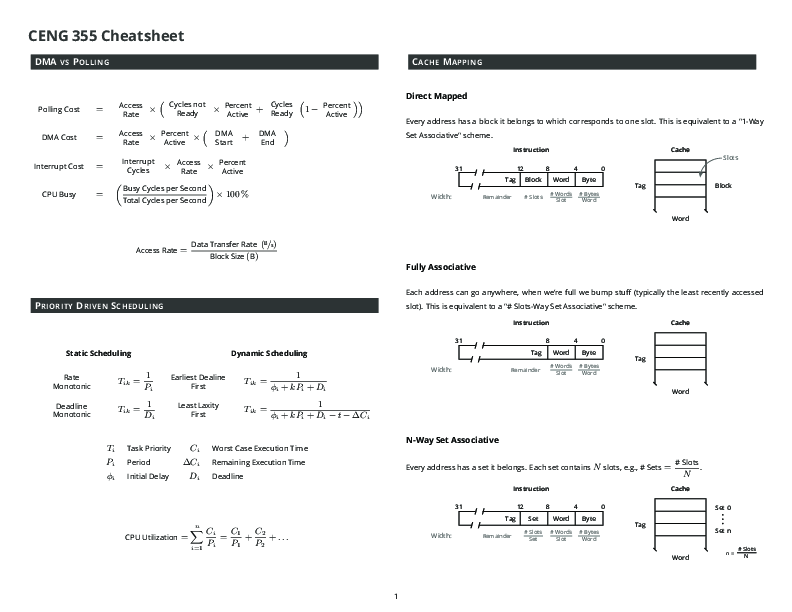
\includegraphics[width=1\linewidth]{CENG355/Ceng355-0.png}
		\caption{Cheatsheet Part 1}
		\label{fig:ceng355-0}
	\end{figure}
	\begin{figure}
		\centering
		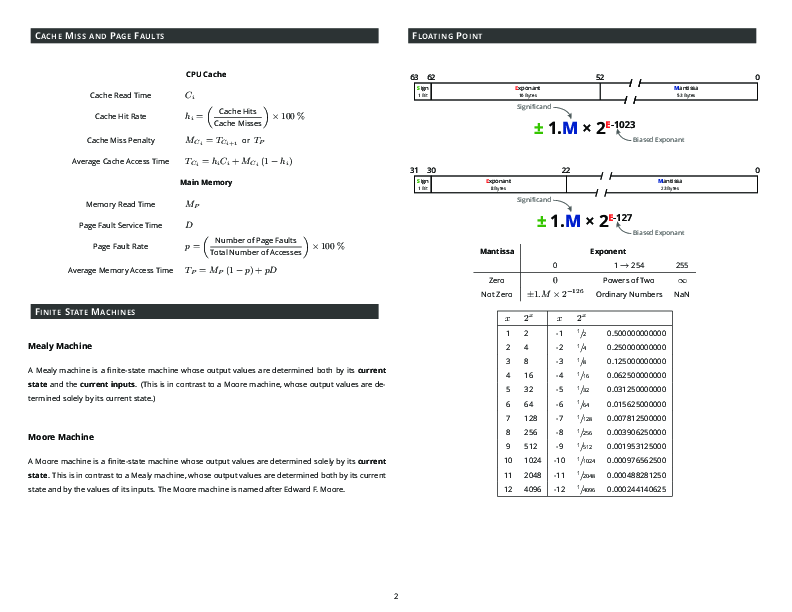
\includegraphics[width=1\linewidth]{CENG355/Ceng355-1.png}
		\caption{CheatSheet Part 2}
		\label{fig:ceng355-1}
	\end{figure}
\begin{multicols}{2}
\section{I/O}
% Create documents for one example from https://www3.nd.edu/~cpoellab/teaching/cse40463/slides4.pdf
\section{Interfacing}
\section{Memory}
\textbf{\underline{Principle of Locality}}:
\hrule
Programs tend to reuse data and instructions near
those they have used recently, or that were recently
referenced themselves. \newline
\textbf{Temporal locality}:
\fcolorbox{byzantine!45}{capri!25}{Recently referenced items are likely to be referenced again in the near future}
\textbf{Spatial locality}:
\fcolorbox{blizzardblue!85}{burlywood!25}{Items with nearby addresses tend to be referenced close together in time.}
\textbf{Data:}
\begin{itemize}
\item Reference array elements in succession: spatial locality
\item Reference sum each iteration: temporal locality
\end{itemize}
\textbf{Instructions:}
\begin{itemize}
\item Reference instructions in sequence: spatial locality.
\item Cycle through loop repeatedly: temporal locality.
\end{itemize}

\subsubsection{Blocked Matrix Code}
\begin{lstlisting}[language=Java]
void bijk(array A, array B, array C, int n, int bsize)
{
	int i, j, k, kk, jj;
	double sum;
	int en = bsize * (n/bsize); /* Amount that fits evenly into blocks */
	
	for (i = 0; i < n; i++)
	for (j = 0; j < n; j++)
	C[i][j] = 0.0;
	
	for (kk = 0; kk < en; kk += bsize) {
		for (jj = 0; jj < en; jj += bsize) {
			for (i = 0; i < n; i++) {
				for (j = jj; j < jj + bsize; j++) {
					sum = C[i][j];
					for (k = kk; k < kk + bsize; k++) {
						sum += A[i][k]*B[k][j];
					}
					C[i][j] = sum;
				}
			}
		}
	}
}
\end{lstlisting}
Copy-paste code here to remove the line numbers.
\end{multicols}
\section{Arithmetic}
\begin{figure}
	\centering
	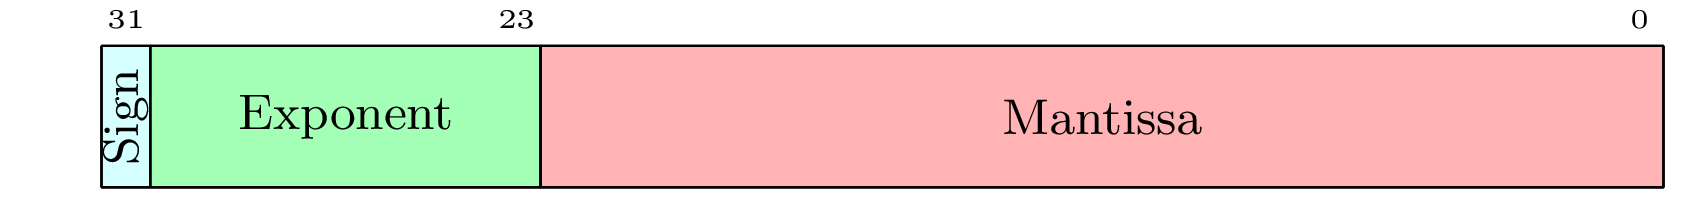
\includegraphics[width=1\linewidth]{CENG355/Exponent.png}
	\caption{IEEE 754 floating point (correct later)}
	\label{fig:exponent}
\end{figure}
\begin{align}
& t_{avg} = h_1C_1 + (1-h_1)(h_2C_2 + (1-h_2)M) \\
& \quad \text{where}  \notag
\end{align}
$h_1$ \textit{is the hit rate in the } $L_1$ \textit{caches.} \newline 
$h_2$ \textit{is the hit rate in the } $L_2$ \textit{ cache.} \newline
$C_1$ \textit{is the time to access information in the } $L_1$ \textit{caches.}\newline
$C_2$ \textit{is the miss penalty to transfer information from the } $L_2$ \text{cache to an } $L_1$ \textit{ cache.} \newline
\textit{M is the miss penalty to transfer information from the main memory to the } $L_2$ \textit{cache.}

\section{Concurrency}

\colorbox{capri!85}{\makebox(12,12){\textcolor{white}{This better work rofl, why is this so damn hard}}}
\setlength{\fboxrule}{6pt}%
\fcolorbox{blizzardblue!85}{carrotorange!85}{Fun with colour} 

\begin{align*}
& \text{Amdahl's Law} =  \frac{1}{f_{unenh} + f_{enh}/p}
\end{align*}

\begin{figure}
	\centering
	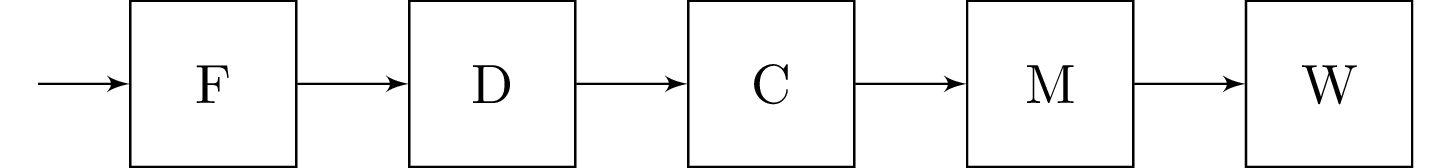
\includegraphics[width=1\linewidth]{CENG355/Pipeline.png}
	\caption{Pipeline for Question 2}
	\label{fig:q2diagram}
\end{figure}

%%% Manually modify after exams or before the test hits me
\chapter{CENG356}
\textbf{Increm­ental vs Iterative}

\begin{longtable}[]{@{}ll@{}}
	\toprule
	Increm­ental & Iterative\tabularnewline
	\midrule
	\endhead
	1. The requir­ements are divided into different builds & 1. Does not
	start with a full specif­ication\tabularnewline
	2. Needs a clear and complete definition of the whole system from the
	start & 2. Building and improving the product step by
	step\tabularnewline
	3. Customers can respond to each build (but a build may not represent
	the whole system) & 3. We can get reliable user feedback\tabularnewline
	4. Increm­ental fundam­entally means~\textbf{add onto}~and helps you to
	improve your~\textbf{proc­ess} & 4. Good for big projects\tabularnewline
	~ & 5. Only major reqs. can be defined, details may evolve over
	time\tabularnewline
	~ & 6. Iterative fundam­entally means~\textbf{redo}~and helps you to
	improve you~\textbf{prod­uct}\tabularnewline
	\bottomrule
\end{longtable}

\textbf{Protot­yping}\label{prototyping}

\begin{longtable}[]{@{}l@{}}
	\toprule
	\vtop{\hbox{\strut \textbf{Types of
				Protot­ypes:}}\hbox{\strut \emph{Throw­away}~= Example is a paper one.
			Will be used only for evalua­tion;~\emph{Incre­mental}~= created a
			separate compon­ents;~\emph{Evolu­tio­nary}~= refined to become actual
			product}\hbox{\strut \textbf{Prot­otype
				Fideli­ty:}}\hbox{\strut \emph{Low}~= Omit details (Rough, no code, easy
			to trash) - Paper, Storyb­oard, Wizard of OZ (evalu­ation)~\emph{High}~=
			Looks like a polished product (looks of product, comment on aesthe­tics,
			GUI powerpoint etc are used)}\hbox{\strut \textbf{Prot­otyping can help
				answer:}}\hbox{\strut - Crowded UI, Knobs versu slider for contro­lling
			volume, Navigation = Transp­arent or solid menu?}}\tabularnewline
	\bottomrule
\end{longtable}

\textbf{White Box/Black Box
	Testing}\label{white-boxblack-box-testing}

\begin{longtable}[]{@{}l@{}}
	\toprule
	\vtop{\hbox{\strut \textbf{White}~= AKA glass box, struct­ural; Tester
			know the source code and can debug at runtime = Develo­per's
			perspe­ctive}\hbox{\strut \textbf{Unit Testing}~= Do discrete parts of
			my system work as expected?}\hbox{\strut - Does an individual method
			work as expected?}\hbox{\strut - Necessary calls to other methods should
			be mocked out where possible}\hbox{\strut -Always white
			box}\hbox{\strut \textbf{Black}~= Tester gives inputs and observe
			outputs (No code, only focus on reqs., interacts with UI only) = User's
			perspe­ctive}\hbox{\strut \textbf{Acce­ptance Testing}~= Is the system
			working from the customer's perspe­­ctive? (AKA. System
			testing)}\hbox{\strut - Interacts with system through GUI}\hbox{\strut -
			Focused in feature~}\hbox{\strut Usually black box}}\tabularnewline
	\bottomrule
\end{longtable}

White = Did we build the system right?\\
Black = Did we build the right system?

\textbf{Agile vs TDD}\label{agile-vs-tdd}

\begin{longtable}[]{@{}l@{}}
	\toprule
	\vtop{\hbox{\strut \textbf{TDD}~= focused on how code gets written (for
			work cycles of indivi­duals or small groups of developers
			exclus­ively)}\hbox{\strut \textbf{Agile}~= Overall develo­pment process
			(focuses on project management and groups of develo­pers, as opposed to
			specif­ically how a given developer writes code)}}\tabularnewline
	\bottomrule
\end{longtable}

\textbf{Polymo­rphism}\label{polymorphism}

\begin{longtable}[]{@{}l@{}}
	\toprule
	A property of OO software by which an abstract operation may be
	performed in different ways, typically in different
	classes.\tabularnewline
	\bottomrule
\end{longtable}

\textbf{Inheri­tance}\label{inheritance}

\begin{longtable}[]{@{}l@{}}
	\toprule
	Implicit possession by a subclass of features defined in a subclass.
	Features include variables and methods\tabularnewline
	\bottomrule
\end{longtable}

\textbf{Abstract Classes and Abstract
	Operations}\label{abstract-classes-and-abstract-operations}

\begin{longtable}[]{@{}ll@{}}
	\toprule
	Abstract Operations & No method for that operation exists in the
	class\tabularnewline
	\midrule
	\endhead
	Abstract Class & Cannot have any instances\tabularnewline
	\bottomrule
\end{longtable}

- A class that has one or more abstract more abstract methods must be
declared abstract.\\
- Any class, except a leaf class, can be declared abstract\\
- Label with \textless{}ab­str­act\textgreater{}

\textbf{Sturctural Modelling}\label{sturctural-modelling}

\begin{longtable}[]{@{}l@{}}
	\toprule
	\textbf{Gene­ral­iza­tion:}~Specia­lizing a superclass into subcla­sses.
	Avoid unnece­ssary genera­liz­ations\tabularnewline
	\midrule
	\endhead
	\textbf{Depe­nde­ncy:}~Used for extremely weak relati­­on­ships between
	classes. Ex. A class makes use of a library\tabularnewline
	\textbf{Aggr­ega­tion:}~Represents "­par­t-w­hol­e" relati­ons­hips. The
	whole side is called the aggregate. Aggreg­ations are read as "is part
	of"\tabularnewline
	\textbf{Comp­osi­tion:}~Are strong forms of aggreg­ation. If the
	aggregate is destroyed, then the parts are also
	destroyed.\tabularnewline
	\bottomrule
\end{longtable}

\textbf{Aggr­ega­tion}~= An associ­ation is an aggreg­ation if: the
parts 'are part of' the aggregate. The aggregate 'is composed of' the
parts. When something owns or controls the aggregate, then they also own
and control the parts

\textbf{Software Archit­ecture}\label{software-architecture}

\begin{longtable}[]{@{}l@{}}
	\toprule
	Process of designing the global organi­zation of a software system
	including:\tabularnewline
	\midrule
	\endhead
	- Dividing software into subsystems - Deciding how these will interact -
	Determ­ining their interf­aces: the archit­ecture is the core of the
	design so all software engineers must understand it. Archit­ecture will
	often constrain the overall effici­ency, reusab­ility and
	mainta­ina­bility of the system\tabularnewline
	Import­ance: To enable everyone to better understand the system, To
	allow people to work on individual pieces of the system in isolation,
	prepare for extension of the system, facilitate reuse and
	reusab­ility\tabularnewline
	Archit­ecture in different views:\tabularnewline
	- Logical breakdown into subsys­tems, - Interfaces among the
	subsys­tems, - Dynamics of the intera­ction among components at run
	time, - Data will be shared among subsys­tems, - Components will exist
	at run time and the machines or devices on which they will be located,
	-\tabularnewline
	Ensuring mainta­ina­bility and reliab­ility = archit­ectural model is
	stable\tabularnewline
	- Stable = means new features can be easily added with only small
	changes to the archit­ecture\tabularnewline
	\bottomrule
\end{longtable}

\textbf{Agile vs. Spiral}\label{agile-vs.-spiral}

\begin{longtable}[]{@{}ll@{}}
	\toprule
	Agile & Spiral\tabularnewline
	\midrule
	\endhead
	Iterations are shorter (1 to 4 weeks) & Iterations are longer (4 to 6
	months)\tabularnewline
	Not good for low rates of requir­ements change (cost of collab­ora­tion)
	& Suitable for large scale develo­pment (due to risk
	analysis)\tabularnewline
	Is good for low-risk and less critical systems & More emphasis on
	docume­ntation and process\tabularnewline
	\bottomrule
\end{longtable}

Both are increm­ental and iterative

\textbf{Static vs Dynamic
	Testing}\label{static-vs-dynamic-testing}

\begin{longtable}[]{@{}llll@{}}
	\toprule
	Static & Dynamic & Validation & Verifi­cation\tabularnewline
	\midrule
	\endhead
	Objective = Finding errors in early stages of the develo­pment cycle &
	Objective = Checks the functional behaviour of the system & Check that
	the software product meets the customer's actual needs & Whether the
	system is well-e­ngi­neered? Error free?\tabularnewline
	Are we building the product right? & Are we building the right product?
	& Dynamic & Static\tabularnewline
	Activities = Reviews, Walkth­roughs, Inspection & Testing - The product
	meets the user's needs = the product fulfills its intended
	use\tabularnewline
	The product is built according to the reqs.\tabularnewline
	\bottomrule
\end{longtable}

Checking whether the software is of high quality will not ensure that
the system is useful. So~\textbf{Trust but verify, verify but also
	valida­te}.

\textbf{Race Conditions}\label{race-conditions}

\begin{longtable}[]{@{}l@{}}
	\toprule
	A race occurs when two threads are using the same resources and the
	order of operations is important\tabularnewline
	\midrule
	\endhead
	Critical races can be prevented by locking data so they cannot be
	accessed by other threads\tabularnewline
	Ex. A keyword like~\emph{synch­ron­ized}\tabularnewline
	\bottomrule
\end{longtable}

\textbf{Testing Strate­gies}\\
- Hard to test critical races\\
- Use mocking to control the order

\textbf{UML Diagrams}\label{uml-diagrams}

\begin{longtable}[]{@{}l@{}}
	\toprule
	\textbf{Inte­raction Diagra­ms:}~A set of diagrams to model the dynamic
	aspects of the system. To visualize how the system runs. Often built
	from a use case and class diagram to illustrate how a set of objects
	accomplish the required intera­ctions with an actor.\tabularnewline
	\midrule
	\endhead
	\textbf{Sequence Diagra­ms:}~An intera­ction diagram that focuses on the
	sequence of messages exchanged by a set of objects performing a certain
	task\tabularnewline
	\textbf{Comm­uni­cation Diagra­ms:}~Emphasize how objects collab­orate
	to realize an intera­ction\tabularnewline
	\textbf{State Diagrams}~At any given point in time, the system is in
	precisely one state and will remain in the state until an event occurs
	to change state. Is a directed graph, nodes are states, edges are
	transi­tions. Have timeouts to automa­tically change
	states\tabularnewline
	\bottomrule
\end{longtable}

\textbf{Inte­raction Diagrams Show (Inter­act­ion)}~= the steps of the
use case, the steps of a piece of functi­ona­lity. Composed of instances
of classes, actors and messages.~\\
\textbf{Sequence Diagra­ms:}~Can represent condit­ional logic and loops
and show explicit destru­ction of objects.\\
\textbf{Comm­uni­cation Diagram:}~Annota­tions of object diagrams. Shows
link between objects that commun­icate

\textbf{Functional vs.
	Non-fu­nct­ional}\label{functional-vs.-non-functional}

\begin{longtable}[]{@{}ll@{}}
	\toprule
	Functional & What is the system doing? For example: Should be able to
	make two slides\tabularnewline
	\midrule
	\endhead
	Non Functional & How is the system doing a thing? For Ex. A created
	slide should be displayed in 1 second\tabularnewline
	\bottomrule
\end{longtable}

\textbf{Non - Functional}\label{non---functional}

\begin{longtable}[]{@{}l@{}}
	\toprule
	Response Time, Throug­hput, Resource Usage, Reliab­ility, Availa­bility,
	Failure Recovery, Mainta­ina­bility, Modula­rity, Security,
	Testab­ility, Learna­bility, Usability, Price, Extens­ibi­lity,
	Reusab­ility\tabularnewline
	\bottomrule
\end{longtable}

Non functional requir­ements may be more critical than functional
requir­ements, if these are not met, the system is useless! Usually
cannot be implem­ented in a single module of a program.

\textbf{The Process of Design}\label{the-process-of-design}

\begin{longtable}[]{@{}l@{}}
	\toprule
	\vtop{\hbox{\strut \textbf{Design}~= problem solving process to find and
			describe a way:}\hbox{\strut - to implement the system's functional
			reqs.~}\hbox{\strut - respect the constr­aints imposed by
			non-fu­nct­ional reqs. (budget, deadli­nes..)}\hbox{\strut - adhere to
			general principles of good quality}\hbox{\strut \textbf{Design Issues}~=
			sub problems of the overall design. Each issue has several altern­ative
			solutions. The designer makes a design decision to resolve each issue.
			This involves choosing what he or she consider to be the best option
			from among the altern­atives.~}\hbox{\strut \textbf{Good design}~=
			increasing profit with reduced cost, ensure confor­mation to the reqs.,
			accele­rating develo­pment, increasing usability, effici­ency,
			reliab­ility, mainta­ina­bility and reusab­ility}}\tabularnewline
	\bottomrule
\end{longtable}

They use knowledge of the reqs., the design created so far, the tech.
available, software design principles and 'best practices' and past
experi­ences.
%\import{ELEC460/}{elec460Formulas.tex}

\chapter{Glossary}
\printglossary[title=Glossary]
\begin{lstlisting}
	Consider using a manual approach to style listlisting, 
	what I do for pandoc, a combination of prism.js with <pre> and <code> tags inbewteen.
\end{lstlisting}

\chapter{ELEC 460: Control Theory II}


\textbf{Necessary and Sufficient Condition for Stability} \newline

\begin{enumerate}
\item $|a_n| < |a_0|$ 
\item $P(1) > 0$
\item \begin{align*}
P(-1) & > 0 \ \text{for n even } \\
& < 0 \ \text{for n odd}
\end{align*}
\item $b_{n-1}> |b_0|, |c_{n-2}|>|c_0|, \cdots |q_2| > |q_0|$
\end{enumerate}

\textbf{Special Case n =2} \newline 
$P(z) =a_0z^2+a_1z+a_2$ \newline 
\begin{tabular}{c c c}
$z^0$ & $z^1$& $z^2$ \\
$a_2$ & $a_1$ & $a_0$
\end{tabular} \newline
$P(z) \neq 0$ for $|z| \geq 1$ if and only if 
\begin{enumerate}
\item $|a_2| < |a_0|$
\item $P(1) > 0$
\item $P(-1) > 0 \quad (n=2)$
\end{enumerate}

 \textbf{Root Locus} presents the poles of the closed loop system when the gain K changes from zero to infinity.

 \textbf{Construction of the Root Locus}

 Open loop transfer function
 $ \displaystyle \text{KH}\left( s \right)G\left( s \right) = K\frac{B(s)}{A(s)}$

m: the order of the \textbf{open-loop} numerator polynomial.

 n: the order of the \textbf{open-loop} denominator polynomial. $q=n-m$

 \textbf{Rule 1:} number of branches equals the number of poles of the
 open-loop transfer function

 \textbf{Rule 2:} If the total number of poles and zeros of the open-loop
 system to the right of the s-point on the real axis is odd, then this
 point lies on the locus.

\textbf{Rule 3:} The locus starting point (K=0) are at the open-loop
 poles and the locus ending points (K=$\infty$) are at the open loop zeros and
 n-m branches terminate at infinity.

\textbf{Rule 4 and 5:} Slope of asymptotes of root locus as `s' approaches infinity. \newline Abscissa of the intersection between asymptotes of root locus and real-axis.
\begin{align*}
& \sigma  = {\frac{\sum\limits_{i = 1}^n {{p_i}}  - \sum\limits_{i = 1}^m {{z_i}} }{q}} \quad \theta = \pm r{\frac{180}{q}} \quad \text{where r=1, 3, 5} \\
& f\left( s \right) = A\left( s \right) + KB\left( s \right) = 0\ \ \ \ and\ \ \ \ K = - \frac{A\left( s \right)}{B\left( s \right)} \\
& \frac{\text{dK}}{\text{ds}} = - \frac{A^{'}\left( s \right)B\left( s \right) - A\left( s \right)B^{'}\left( s \right)}{B^{2}\left( s \right)} = 0 \\
 \end{align*}
 \textbf{Rule 5:} 

 \textbf{Rule 6:} Break-away and break-in points. From the characteristic
  equation

  \[f\left( s \right) = A\left( s \right) + KB\left( s \right) = 0\ \ \ \ and\ \ \ \ K = - \frac{A\left( s \right)}{B\left( s \right)}\]

  The break-away and break-in points can be found from

  \[\frac{\text{dK}}{\text{ds}} = - \frac{A^{'}\left( s \right)B\left( s \right) - A\left( s \right)B^{'}\left( s \right)}{B^{2}\left( s \right)} = 0 \]

  \textbf{Rule 7:} Angle of departure from complex poles or zeros.
  Subtract from $180^o$ the sum of all angles from all other zeros and poles
  of the open-loop system to the complex pole (or zero) with appropriate signs. 

 \begin{align*}
& \text{Z-transform: Definition} \quad F(z)=Z[f(t)]-Z[f(kT)]=\sum_{k=0}^{\infty}f(kT)z^{-k} \\
& e^\ast(\infty)=\lim_{z \rightarrow 1} (1-z^{-1})E(z) \quad K_p=\lim_{z \rightarrow 1} GH(z), \quad e^\ast (\infty) = \frac{1}{1+K_p} \\
& e^\ast(\infty) = \frac{1}{K_v}, \quad K_v =  \lim_{z \rightarrow 1} \frac{(1-z^{-1}) GH(z)}{T}  \\
& e^\ast(\infty) = \frac{1}{K_a}, \quad K_a =  \lim_{z \rightarrow 1}\frac{(1-z^{-1})^2 GH(z)}{T^2}
\end{align*}

{\bf Linear Factor Rule.}  
 For each factor of $Q$ of the form $(ax+b)^m$, 
 the partial fraction decomposition contains 
 the following sum of $m$ partial fractions:  
\[
\frac{A_1}{ax+b} + \frac{A_2}{(ax+b)^2} + \cdots + \frac{A_m}{(ax+b)^m},
\]
 where the $A_i$ are constants to be determined.  

\medskip
\noindent
{\bf Quadratic Factor Rule.}  
 For each factor of $Q$ of the form $(ax^2+bx+c)^m$, 
 where $ax^2+bx+c$ is an irreducible quadratic, 
% the partial fraction decomposition contains 
 the following sum of $m$ partial fractions:  
\[
\frac{A_1x+B_1}{ax^2+bx+c} + \frac{A_2x+B_2}{(ax^2+bx+c)^2} + \cdots 
  + \frac{A_mx+B_m}{(ax^2+bx+c)^m},
\]
 where the $A_i$ and $B_i$ are constants to be determined. 


Geometric Sum $\sum\limits_{k = -N}^{N} {ar^{k - 1} = a\frac{1-r^{N}}{{1 - r}}} \sum_{i=0}^\infty a^i=\frac{1}{1-a}$

$ x(k+2)-\frac{3}{2}x(k+1)+\frac{1}{2}x(k)=u(k), \text(x(0)=1,x(1)=5/2) $

$[z^2X(z)-z^2x(0)-zx(1)]-\frac{3}{2}(zX(z)-zx(0)]+\frac{1}{2}X(z)=\frac{z}{z-1}$


\textbf{Effects of T on Transient Behaviour} \hfill \break 
$s= -\zeta \omega_n \pm j \omega_n \sqrt{1-\zeta^2}$,  \hfill \break 
$\zeta$: damping ratio  \hfill \break 
$\omega_n$: undamped natural frequency,  \hfill \break 
$\omega_d$: damped natural frequency \hfill \break
$z=e^{Ts} \rightarrow z= \exp\left[T(-\zeta \omega_n +j\omega_n \sqrt{1-\zeta^2})\right]$, and
$|z|=e^{-T \zeta \omega_n}$, $\angle z = T \omega_n \sqrt{1-\zeta^2}= T \omega_d$. $\uparrow T$ makes system less stable (for the same gain K) than $\downarrow T$.
\textbf{Matrix Inverses for 2x2 and 3x3}
\begin{align*}
& A^{-1} = \begin{bmatrix}
a & b \\
c & d
\end{bmatrix}^{-1}= \frac{1}{|A|}\begin{bmatrix}
d & -b \\
-c & a
\end{bmatrix} \ \begin{bmatrix}
a & b & c \\
d & e & f \\
g & h & i
\end{bmatrix}^{-1} \\
& A^{-1} = 
\frac{1}{|A|}\begin{bmatrix}
% Row one determinate
+\begin{vmatrix}
e & f \\
h & i
\end{vmatrix} & 
-\begin{vmatrix}
b & c \\
h & i
\end{vmatrix} & 
+\begin{vmatrix}
b & c \\
e & f
\end{vmatrix} \\
& & \\
-\begin{vmatrix}
d & f \\
g & i
\end{vmatrix} & +\begin{vmatrix}
a & c \\
g & i
\end{vmatrix} &
-\begin{vmatrix}
a & c \\
d & f
\end{vmatrix} \\
& & \\
+\begin{vmatrix}
d & e \\
g & h
\end{vmatrix} &
-\begin{vmatrix}
a & b \\
g & h
\end{vmatrix} &
+\begin{vmatrix}
a & b \\
d & e
\end{vmatrix}
\end{bmatrix}^{-1}
\end{align*}
\textbf{Bilinear Transform}  \hfill \nopagebreak
$s= \frac{2(1-z^{-1})}{T(1+z^{-1})}$, $z=\cfrac{1+0.5Ts}{1-0.5Ts}$.

\text{1. Stability} $\Re[s] < 0$

$\displaystyle \Re \left(\frac{2}{T} \frac{1-z^{-1}}{1+z^{-1}}\right)= \Re \left(\frac{2}{T}\frac{z-1}{z+1}\right) < 0$, $z= \sigma + j \omega$ \hfill \nopagebreak

$\displaystyle \Re \frac{z-1}{z+1}=\Re \left[\frac{\sigma^2-1+\omega^2+2j\omega}{(\sigma+1)^2+\omega^2}\right] \rightarrow \sigma^2-1+\omega^2 < 0$.


\textbf{Solution of inhomogeneous state equations}
scalar $\dot{x}=ax+bu \quad \dot{x}-ax=bu$
\begin{align*}
& e^{-at}[\dot{x}(t)-ax(t)]=\underbrace{\frac{d}{dt}[e^{-at}x(t)]=e^{-at}bu(t)}_{\text{integrate ~$0 \rightarrow t$}} \\
& e^{-at}x(t)-x(0) = \int^t_0 e^{-a \tau}bu(\tau) d\tau \\
& \rightarrow x(t)=e^{at}x(0)+e^{at}\int_0^te^{-a\tau}bu(\tau)d\tau
\end{align*}
matrix: $\dot(x)=Ax+bu$, but taking $\mathcal{L}^{-1}$ leads to  \hfill \break  $x(t)=e^{At}x(0)+\int_{0}^{t}e^{A(t-\tau)}bu(\tau) d\tau$

\textbf{Controllable Canonical Form} \hfill \nopagebreak

% \hfill \break \nopagebreak
\resizebox{.9\linewidth}{!}{
  \begin{minipage}{\linewidth}
\begin{align*}
& G(z) = \frac{b_0+b_1z^{-1}+ \cdots + b_nz^{-n}}{1+a_1z^{-1}+ \cdots + a_n}= \frac{b_0z^n+b_1z^{n-1}+ \cdots + b_n}{z^n+a_1z^{n-1}+\cdots + a_n} \\
& G(z)= b_0 + \frac{(b_1-a_1b_0)z^{-1}+(b_2-a_2b_0)z^{-2}+ \cdots + (b_n-a_nb_0)z^{-n-1}}{1+a_1z^{-1}+a_2z^{-2}+ \cdots + a_nz^{-n}} \\
& \begin{bmatrix}
x_1(k+1) \\
 \vdots \\
x_n(k+1)
\end{bmatrix}= \begin{bmatrix}
0      & 1         & 0      & \cdots \\
\vdots & \cdots    &        & \vdots \\
\vdots &           &  \cdots      &   1    \\
-a_n   &  \cdots   & \cdots & -a_1
\end{bmatrix}\begin{bmatrix}
x_1(k) \\
 \vdots \\
x_n(k)
\end{bmatrix}+\begin{bmatrix}
0 \\
 \vdots \\
0 \\
1
\end{bmatrix}u(k) \\
& y(k) = \begin{bmatrix}
b_n-a_nb_0, & b_{n-1}a_{n-1}b_0, & b_1-a_1b_0
\end{bmatrix} \begin{bmatrix}
x_1(k) \\
\vdots \\
x_n(k)
\end{bmatrix} + b_0 u(k) \\
& z \rightarrow s \quad  zX(z) = \mathcal{Z}[x(k+1)] \quad  sX(s) = \mathcal{L}[x(t)]
\end{align*}
  \end{minipage}
} \hfill \nopagebreak

\textbf{Observable Canonical Form} \hfill \nopagebreak

\resizebox{.9\linewidth}{!}{
  \begin{minipage}{\linewidth}
\begin{align*}
& \begin{bmatrix}
\dot{x_1} \\
 \vdots \\
\dot{x_n}
\end{bmatrix}= \begin{bmatrix}
0      & 0         & 0      & -a_n     \\
1 & \cdots    &        & -a_{n-1} \\
0 &           & \cdots &   \vdots \\
0   &  0   & 1 & -a_1
\end{bmatrix} \begin{bmatrix}
x_1 \\
 \vdots \\
x_n
\end{bmatrix}+\begin{bmatrix}
b_n-a_nb_0 \\
 \vdots \\ 
b_1-a_1b_0
\end{bmatrix}u(k) \\
& y(k) = \begin{bmatrix}
0, & \cdots & \cdots, & 0, & 1 
\end{bmatrix} \begin{bmatrix}
x_1 \\
\vdots \\
x_n
\end{bmatrix} + b_0 u(k) 
\end{align*}
  \end{minipage}
} \hfill \nopagebreak

\textbf{Part-Frac-Expansion Method, Dia Canonical} %\hfill \nopagebreak
\vspace{-0.425cm}
\begin{align*}
& G(z) =  b_0 + \frac{c_1}{z-p_1} + \cdots \ \cdots + \frac{c_n}{z-p_n} \\
& \begin{bmatrix}
x_1(k+1) \\
\vdots \\
\vdots \\
x_n(k+1)
\end{bmatrix} =  \begin{bmatrix}
p_1     & 0       & \cdots  & 0      \\
0       & \vdots  &         & 0      \\
\vdots  &         &  \vdots & \vdots \\
0       & 0       &  \cdots & p_n
\end{bmatrix}\begin{bmatrix}
x_1(k) \\
\vdots \\
\vdots \\
x_n(k)
\end{bmatrix} + \begin{bmatrix}
1 \\
1 \\
\vdots \\
1
\end{bmatrix} u(k) \\
&  y(k) = \begin{bmatrix}
c_1 & \cdots & c_n
\end{bmatrix} \begin{bmatrix}
x_1    \\
\vdots \\
x_n
\end{bmatrix} + b_0 u(k)
\end{align*}

\textbf{Special Case} %hill \nopagebreak
%
\vspace{-0.425cm}
\begin{align*}
& y^{(n)}+a_1y^{(n-1)}+ \cdots + a_{n-1}y+a_{n}=u \quad \dot{x} = Ax + bu  \\
& x = \begin{bmatrix}
x_1 \\
\vdots \\
\vdots \\
x_n
\end{bmatrix} \quad 
A = \begin{bmatrix}
0      & 1        &  \vdots & \vdots       & 0        \\
0      & 0        &  1      &              & \vdots   \\
\vdots &          &         & \ddots       & \vdots   \\
0      &          &         &              &  1       \\
-a_n   & -a_{n-1} &  \cdots & \cdots       & -a_1 
\end{bmatrix}
\end{align*}

\vspace*{-0.90cm}

\begin{minipage}[h]{0.25\linewidth}
\[
b = \begin{bmatrix}
0 \\
0 \\
\vdots \\
1
\end{bmatrix}
\]
\end{minipage}
\begin{minipage}[h]{0.75\linewidth}
\begin{align*}
& c = [1 \ 0 \ .. \ 0] \ \quad y =cx+du \ \text{and} \ d=0 \\
& Y(s) = [c(sI-A)^{-1}b+d]U(s) \quad \\ 
& \frac{Y(z)}{U(z)} = c(zI-A)^{-1}b+d 
\end{align*}
\end{minipage}
\textbf{Deadbeat Controller and Deadbeat Response}
\vspace*{-0.25cm}
\begin{align*}
& x(k+1)=Gx(k)+Hu(k) \quad u(k)=-Kx(k) \\
& x(k+1)=(G-HK)x(k) \quad x(k)=(G-HK)^kx(0) \\
& x(k) = (G-HK)^kx(0) \quad x(k) =0 \quad \text(for) k \geq \quad q (q \leq n) \\
& \det(zI-G+HK)=z^n \quad N^n =0, \text{N is nilpotent matrix.}
\end{align*}
\vspace*{-0.7cm}

\textbf{Controllability} A system is controllable, if and only if, it is possible to transfer the system state from any arbitrary initial state x(0) to the origin in finite time. initial state x(0) $\rightarrow$ desired state: x(n)=0.%
%
\textbf{Controllability condition for SI continuous systems:} $\det C = \det[b, \ \ Ab, \ \, \cdots, A^{n-1}b] \neq 0$.

\textbf{Observability} A system is observable if any initial state x(0) can be determined from a finite number of output observations. $\det O_c = \det \begin{bmatrix} 
c \\ cA \\ \vdots \\ cA^{n-1} \end{bmatrix} \neq 0$.

\textbf{Continuous State Transition Matrix:} $\phi(t)$,
$\phi(t)=e^{At}= \mathcal{L}^{-1}[(sI-A)^{-1}]$, then $\dot{\phi}(t)=A\phi(t) \quad \phi(0)=I$, $\dot(x)=Ax$ %\hfill \linebreak

Verification: $x(t)=\phi(0)x(0)=Ix(0)$ 
$\dot{x}(t)=\dot{\phi}(t)x(0)=A\phi(t)x(0)=Ax(t)$. 

Properties of $\phi(t)$:
\vspace*{-0.4cm}
\begin{align*}
& 1) \ \ \phi(0)=e^{A0}=I \\
& 2) \ \ \phi(t) = e^{At} = (e^{(-At)})^{-1}=[\phi(-t)]^{-1} \\
& 3) \ \ \phi(t_1+t_2)=\phi(t_1)\phi(t_2)=\phi(t_2)\phi(t_1) \\
& 4) \ \ [\phi(t)]^n = \phi(nt) \\
& 5) \phi(t_0-t_1)\phi(t_1-t_2)=\phi(t_0-t_2)=\phi(-t_1+t_0)\phi(-t_2+t_1) \\
& e^{A(t_0-t_1)}e^{A(t_1-t_2)} = e^{A(t_0-t_2)}=e^{-A(t_1-t_0)}e^{-A(t_2-t_1)}
\end{align*}%
%
\textbf{BIBO Stability}
Output is bounded for any bounded input.
CTS systems : Poles in left half plane, Discrete Systems: poles inside unit circle.

\textbf{INTERNAL ( Also asymptotic stability)}
Def: Equilibrium state:
 Continuous systems: Assume u(t) = 0;
 $\dot{x}_e=0=Ax_e+bu \rightarrow x_e=0$ \hfill \break 
  Discrete systems: Assume u(k) = 0;
 $x_e(k+1)=0=x_e(k)+Gx_e(k) \rightarrow x_e=0$ \hfill \break
\textbf{Def:} A system is asymptotically stable if any initial condition x(0) converges to
the equilibrium state $x_e=0$.
 (It is assumed $u(t) = 0,t \leq0$  or $u(k)=0, k\geq 0$)
 
 \textbf{Condition for asymptotic stability}: \hfill \break CTS $\Re[\lambda_i\{A\}]<0$ \hfill \break Discrete $|\lambda_i 
 \{G\}|$
, all eigenvalues in unit circle

%\newpage 
%\begin{multicols}{3}

$\text{BIBO Stability} \rightarrow \text{Asymptotic Stability (AS)}$ \hfill \break
BIBO Stability \& no pole zero cancellation $\rightarrow $ AS \hfill \break 
%
Eigenvalues of A are the solutions of $\det(I\lambda -A) = 0$, \hfill \break
Poles of G(z) are the zeros of denominator poly. 
$G(z)=d+c(zI-A)^{-1}b$ where $(zI-A)^{-1}=\frac{\text{adj}(zI-A)}{\text{det}(zI-A)}$
% $A_{ij}=(-1)^{i+j} M_{ij}$, (minor $M_{ij}$, $\det$ with deleted i and j rows/col.
% adj A
C: nonsingular if system controllable. If the system is controllable,
any closed-loop poles can be obtained, %i.e any desired transient response characteristics can be obtained
%\begin{comment}
%Adding a comment here, make sure to add in information about the controlleres and go home and study tommorw
%\end{comment}

\textbf{Feed-forward observers} State Observer: $\tilde{X}(k+1)=G\tilde{x}(k)+Hu(k)$
$\tilde{y}(k)=c \tilde{x}(k)$, Observed state: $\tilde{x}(k)$, Observation error: $e(k)=x(k)-\tilde{x}(k)$, $e(k+1)=Ge(k)$, Dynamics of error depend on G \hfill \break 
\textbf{Prediction (full order) observer} where the estimate $\bar{x}(k+1)$ is obtained based on measurements of up to y(k).
\vspace*{-0.2cm}
\begin{align*}
& \bar{x}(k+1)=G\bar{x}(k)+Hu(k)+k_e[y(k)-\bar{y}(k)] \\
& \bar{x}(k+1)=[G-k_e c] \tilde{x}(k)+Hu(k)+k_ecx(k)
\end{align*}
$k_e$ for this observer can be obtained 
using $k_e=O^{-1}\bar{A}^{-1}(\alpha-a)^T$, where \hfill \break 
$\tilde{A}=\begin{bmatrix}
1   & 0 \cdots & \cdots & 0 \\
a_1 & 1 & & \\
\vdots & a_1 & . &  \\
\vdots & . & . & \\
a_{n-1} & a_{n-2} & \cdots & a_1 & 1
\end{bmatrix}$, \hfill \break  lower triangular Toeplitz matrix, A square matrix that is not singular, i.e., one that has a matrix inverse.
\textbf{Current observer} where the estimate is obtained based on measurements
up to $y(k+1)$.
\vspace*{-0.15cm}
\begin{align*}
& \tilde{x}(k+1)=G\tilde{x}(k)+Hu(k)+K_e[y(k+1)-c\tilde{x}(k+1)] \\
& \bar{z}(k+1)=c\bar{x}(k+1)
\end{align*}
\vspace*{-0.15cm}
\textbf{ASYMPTOTIC OBSERVERS 4 CTS
SYS} 
\vspace*{-0.15cm}
\begin{align*}
& \dot{x}(t) = A x(t)+bu(t) \quad x(0-)=x_0 \\
& y(t) = cx(t) \quad t > 0- \\
& O x(0-) = [y(0-), \ \cdots \ y^{n-1}(0-)]
\end{align*}
\textbf{Open-loop Observer}
Use ($\{A,B,c\}$, $\{u(t), t> 0\}$, and $x_0$) $\rightarrow \{x(t),t>0-\}$,

Effects of disturbance $\epsilon$:
$\tilde{x}_0=x_0-\epsilon$, $|\epsilon| \ll |x_0|$, $\tilde{\dot{x}}(t)=A \tilde{x}(t)+bu(t)$, $\tilde{x}(0-)=\tilde{x}_0=x_0-\epsilon$,
$\dot{e}(t)=Ae(t)$, $e(0-)=\epsilon$, A is unstable $e(t) \rightarrow \infty$

\textbf{Closed-loop observer:}
Output Error: $y(t)-\tilde{y}(t)=y(t)-c\tilde{x}(t)=c[x(t)-\tilde{x}(t=ce(t)$, Observer $\tilde{x}(t)=A \tilde{x}(t)+bu(t)+l[y(t)-c\tilde{x}(t)$, $\tilde{x}(t_o)=\tilde{x}_o$ $\tilde{x}_o$ an estimated initial state vector $l$: feedback gain vector.
\textbf{Observer design:}
$l=O^{-1}\tilde{A}^{-1}(\alpha-a)^T$ \hfill \break 
%$\det C = \det[H, \ GH, \ G^2H, \ \cdots, \ G^{n-1}H] \neq 0$, \\ \hfill
%$O_d = \begin{bmatrix}
%c & cG & \vdots & cG^{n-1}
%\end{bmatrix}^T$
%$\dot{\hat{x}}=T^{-1}AT\hat{x} + T^{-1}Bu$, $x = T\hat{x}$,$T=MW$, control matrix $M$, W is like $\tilde{A}$,but with upper triangular Toeplitiz matrix. $Q = (WN\ast)^{-1}$, N is observability matrix, and $x = Q\hat{x}$, $\hat{\dot{x}}= Q^{-1}AQ\hat{x} + Q^{-1}	Bu$,
%\vspace*{-0.1cm}
\textbf{1. Pole Placement CTS}
\setlength{\abovedisplayskip}{0pt}
\setlength{\belowdisplayskip}{0pt}
\setlength{\abovedisplayshortskip}{0pt}
\setlength{\belowdisplayshortskip}{0pt}
%\vspace*{-0.3cm}
\begin{align*}
& \dot{x}(t)=Ax(t)+bu(t) \quad y(t)=cx(t) \\
& a(s) = \det(sI-A)=s^n+a-1s^{n-1}+ \cdots + a_n
\end{align*}
%\vspace*{-0.2cm}
 \noindent Find a feedback gain vector K so that the characteristic polynomial of the resulting closed-loop system is given by the polynomial:
 %\vspace*{-0.2cm}
\begin{align*}
& \alpha(s) =s^n+\alpha_1s^{n-1}+ \cdots + \alpha_n \quad u(t) =hr(t)- Kx(t) \\
& \dot{x}(t) = (A-bK)x(t)+b h r(t) \quad y=cx(t) \\
& \alpha - a = K C \tilde{A}^T \quad K =(\alpha -a)\tilde{A}^{-T} C^{-1}
\end{align*}
 \vspace*{-0.2cm}
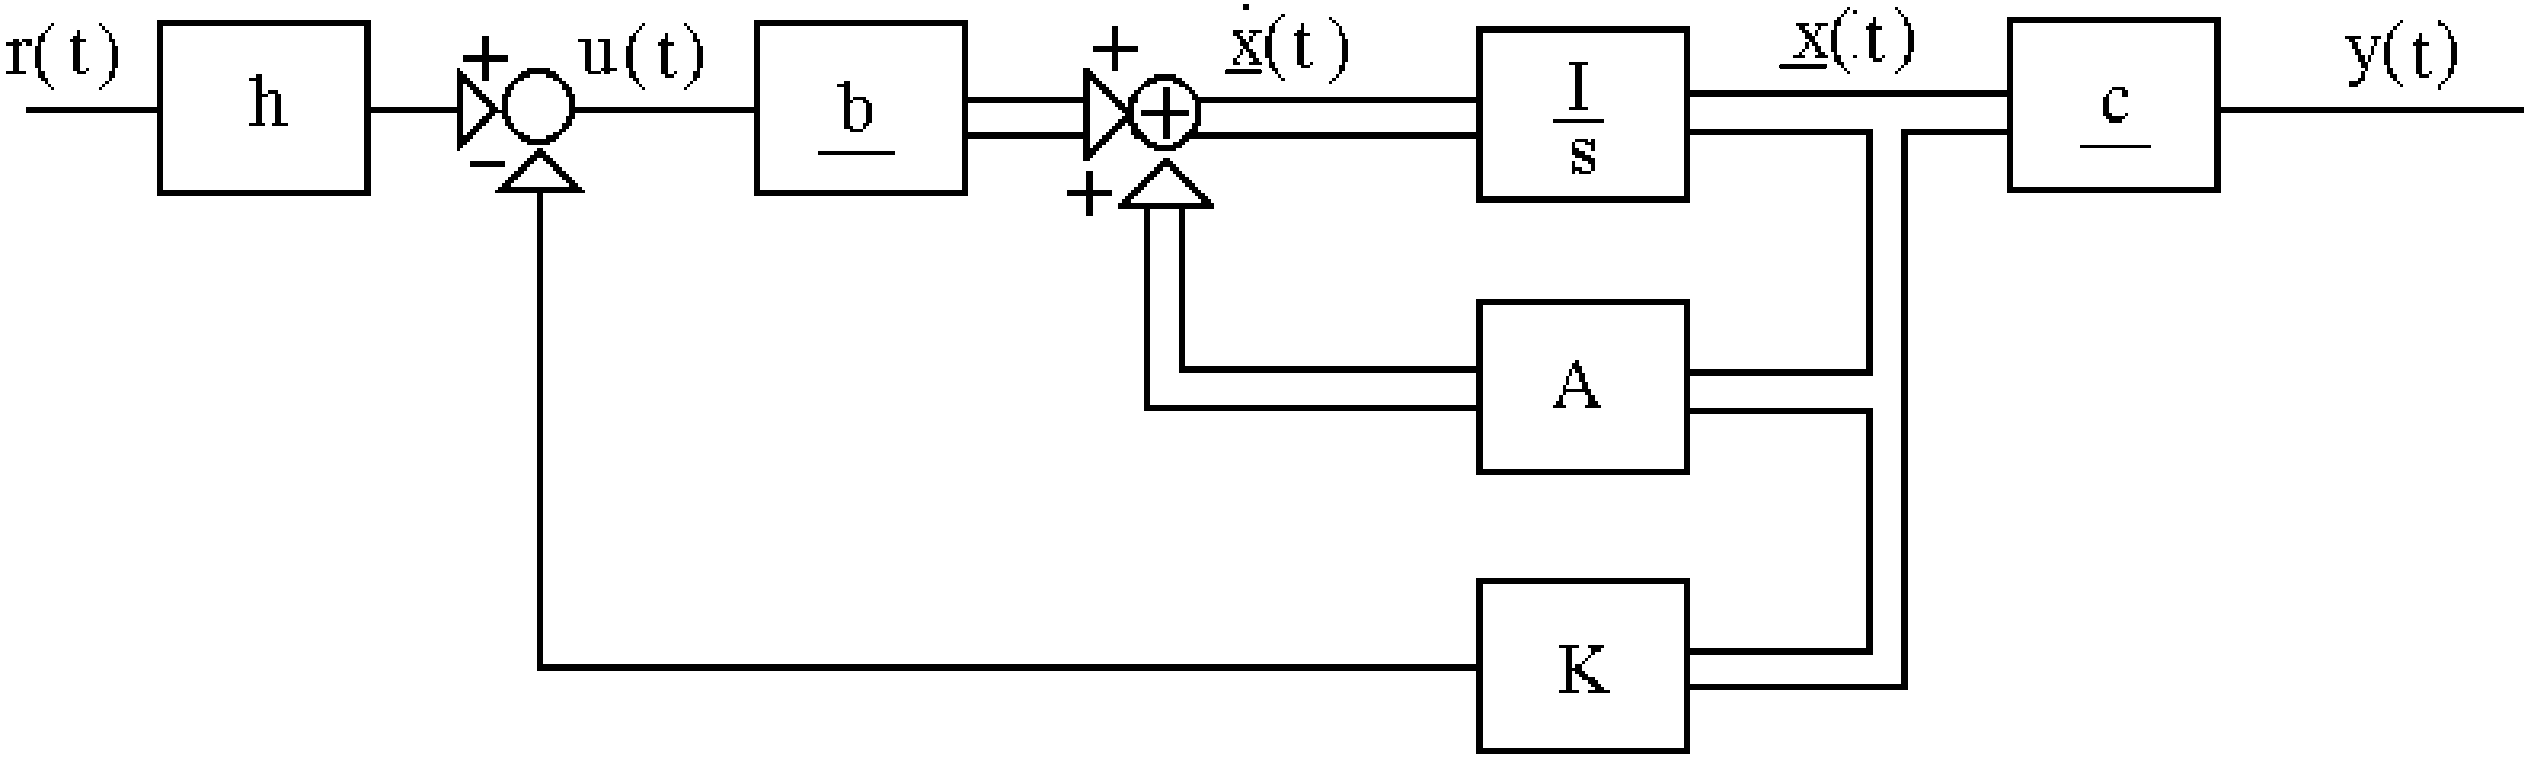
\includegraphics[width=\linewidth]{poleplacementPic.png}
 %\vspace*{-0.2cm}
\textbf{2. Tracking a Reference Signal}
 %\vspace*{-0.2cm}
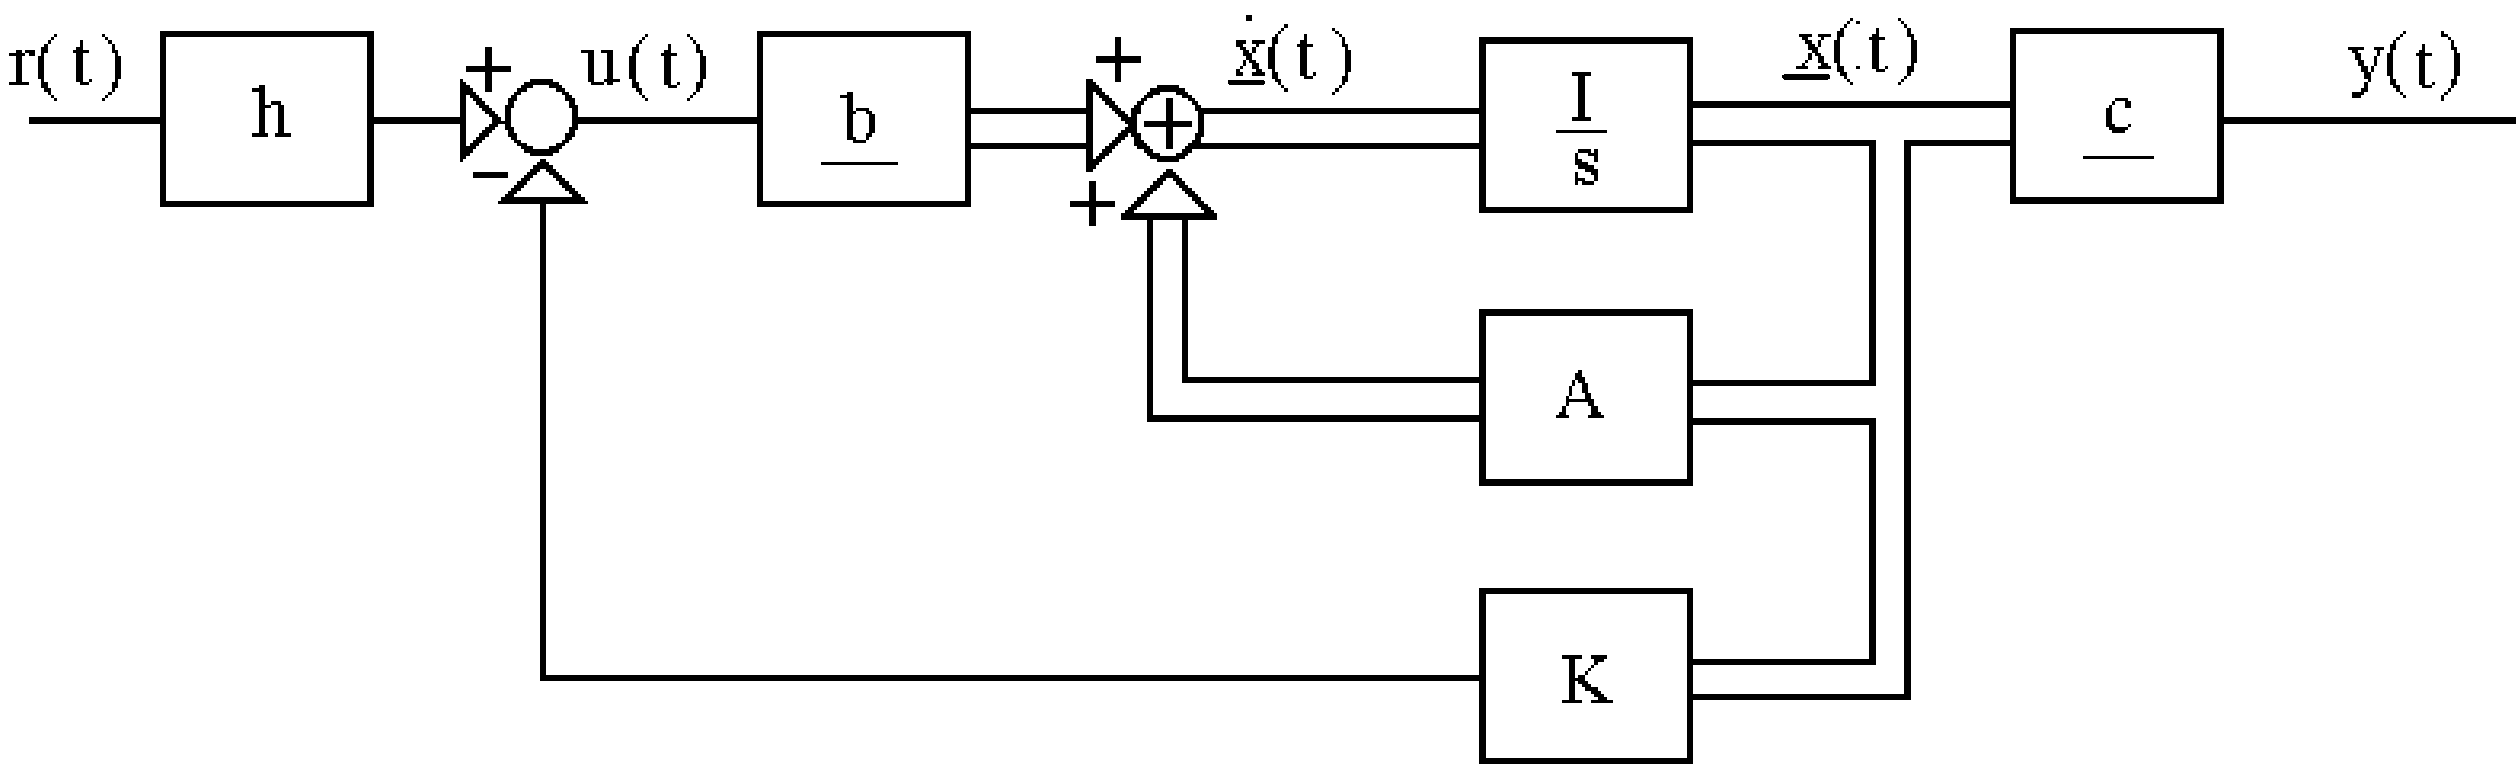
\includegraphics[width=\linewidth]{trackingRefSig.png}
\textbf{Tracking}: y(t) should follow r(t) at steady state(ss)
i.e, y(k) follows r(k) at ss. Find $h$ in $u(k)=hr(k) -Kx(k)$ for tracking. ss $x(k+1)=x(k)$
%\vspace*{-0.2cm}
\begin{align*}
& \dot{x}(t)=Ax+bu=x(t) \downarrow \\
& x(t)=(A-bK)x(t)+bhr(t) \\
& y(t)= c(I-G+HK)^{-1}Hr(t) \quad y(t)=r(t) \\
& h = \frac{-1}{c(A-bK)^{-1}b}
\end{align*}
Estimation of unmeasurable state variables is commonly called observation. $G(s)=C(sI-A)^{-1}B$,
 $\Delta (\lambda)= (\lambda^2+2\zeta \omega_n+ \omega_n^2)(\lambda + \zeta \omega_n)$ \hfill \break 
Overdamped $\zeta > 1$, Critically Damped $\zeta=1$, Underdamped(oscillations) $0< \zeta < 1$
$\zeta = \frac{-\ln(\% OS /100)}{\sqrt{\pi^2 + \ln^2(\% OS /100)}}$
$t_{s} = \frac {4}{\sigma } = \frac {4}{\zeta \omega _{n}}\ \left ( 2\%\ band \right )$,
$t_{s} = \frac {3}{\sigma } = \frac {3}{\zeta \omega _{n}}\ \left ( 5\%\ band \right )$,
% break to make column
\columnbreak
\textbf{Discretization of CTS-Time State Equations:}
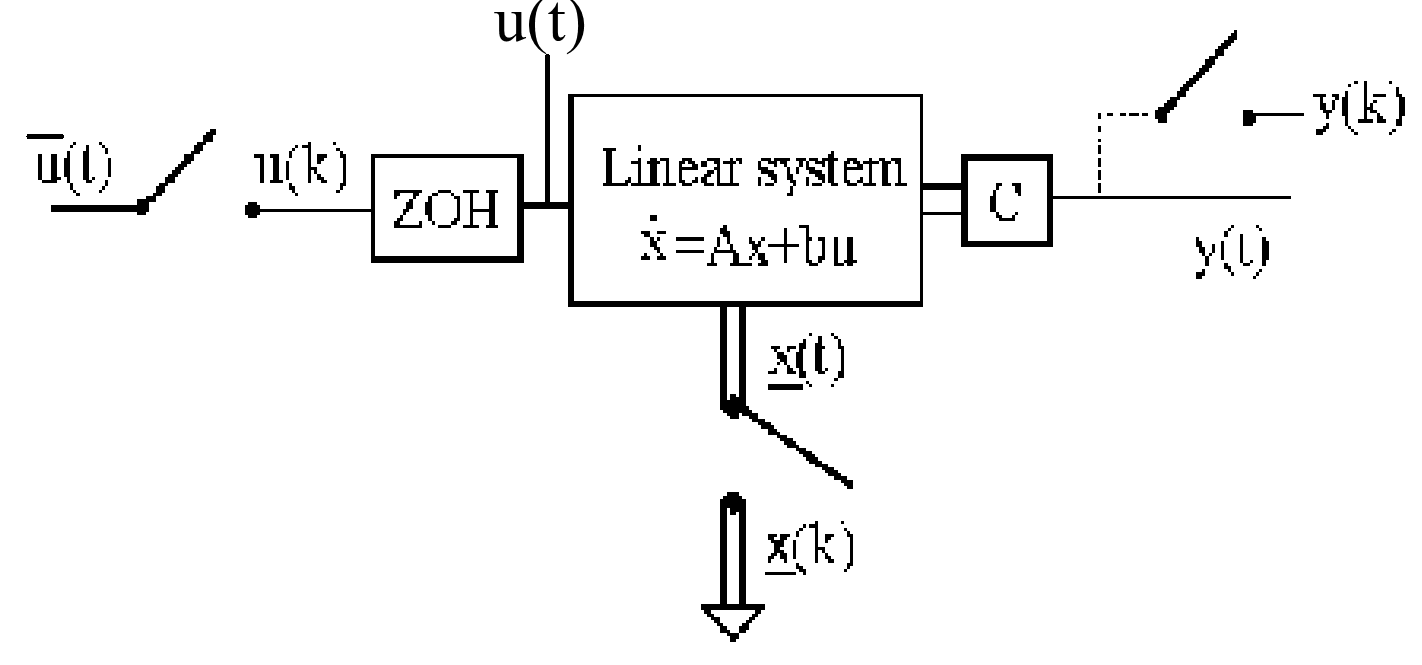
\includegraphics[width=\linewidth]{dis2CTS.png}
%\vspace*{-1.1cm}
\begin{align*}
&  \dot{x}=Ax+bu \quad G(T)=e^{AT}= \phi(T) \ H(T) = (\int_0^T e^{AT} \ dt)b
\end{align*}
%\vspace*{-0.6cm}
\textbf{3. Integral Error Feedback Discrete}
%\vspace*{-0.05cm}
$
x(k+1)=Gx(k)+Hu(k)+w(k) \quad y(k)=c(k)x(k) 
$
w(k) is unknown but constant disturbance.

Problem: Design a state-feedback controller so that
1) The CL eigenvalues are at prescribed locations.

2) The output y(k) follows the reference r(k) for any w(k)
(constant, but unknown) at steady state.

$
 \begin{bmatrix} x(k+1) \\ q(k+1)\end{bmatrix} =
\begin{bmatrix}G & 0 \\ -T_c & 1\end{bmatrix}\begin{bmatrix}x(k) \\ q(k)\end{bmatrix}+
\begin{bmatrix}H \\ 0\end{bmatrix}u(k)+\begin{bmatrix} 0 \\ T\end{bmatrix}r(k)+\begin{bmatrix}w(k) \\ 0\end{bmatrix} \ \
q(k+1)=q(k)+T(r(k)-y(k)) 
$

Find $K = [K_x, K_q]$,$K=(\alpha-a)\tilde{A}^{-T}C^{-1}$,

$ \begin{bmatrix} x(k+1) \\ q(k+1)\end{bmatrix} =
\begin{bmatrix}G-HK_x & -HK_q \\ -T_c & 1\end{bmatrix}\begin{bmatrix}x(k) \\ q(k)\end{bmatrix}+
\begin{bmatrix}0 \\ T\end{bmatrix}u(k)+\begin{bmatrix} 0 \\ T\end{bmatrix}r(k)+\begin{bmatrix}w(k) \\ 0\end{bmatrix}$ $u(k)=-[K_x, K_q]\begin{bmatrix} x(k) \\ q(k)
\end{bmatrix}$ %\hfill \break %using a(z) as given  given characteristic polynomial, and $\alpha(z)$ as desired ch. eqn. \hfill \break 
%\begin{minipage}[h]{1\linewidth}
%\textbf{Discrete} \hfill \break 


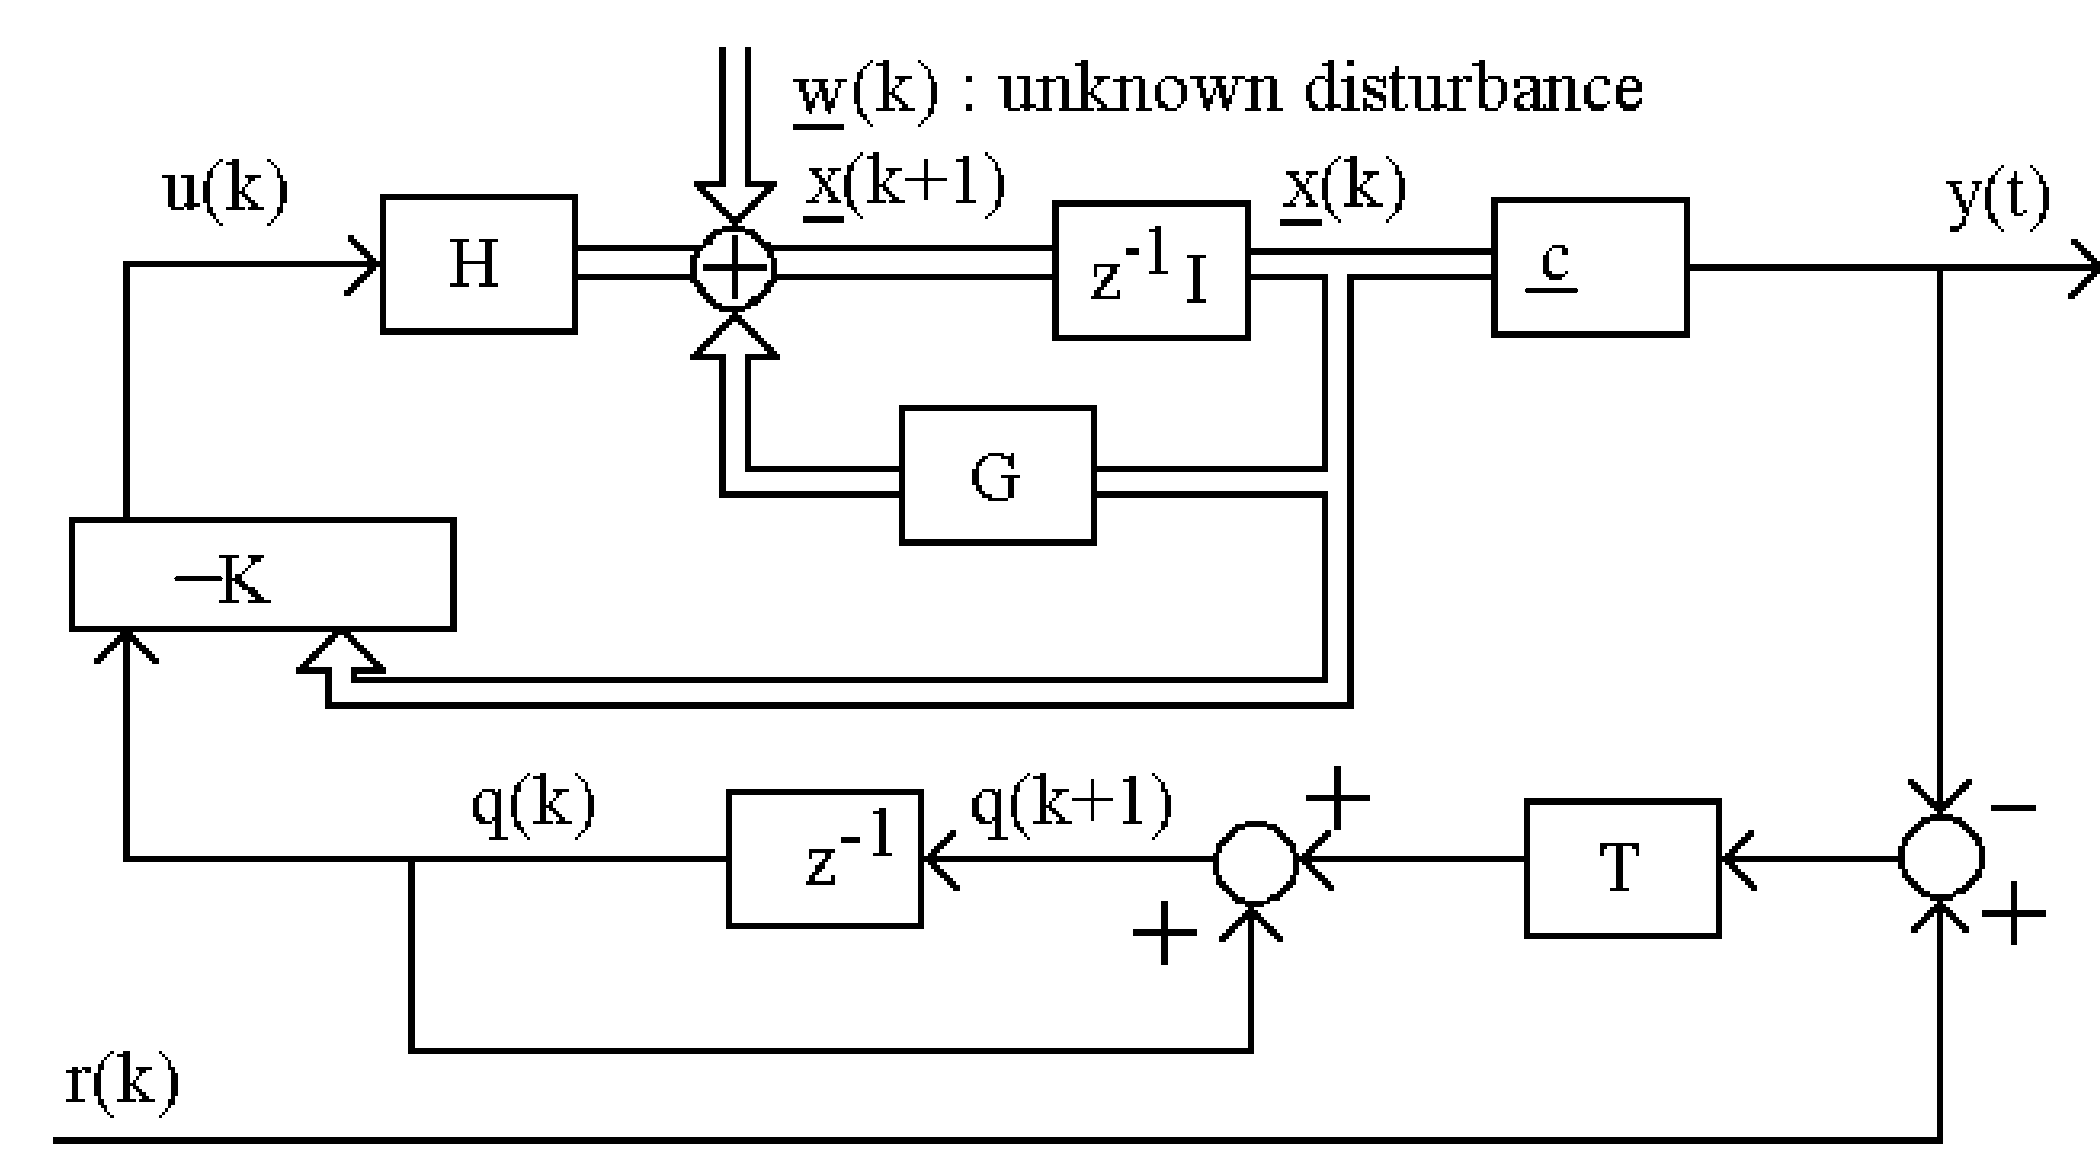
\includegraphics[width=\linewidth]{DiscreteIntegralTracking.png}
%\end{minipage}
%\begin{minipage}[h]{1\linewidth}
%\textbf{Continuous}
\textbf{3. Integral Error Feedback CTS} 

$ \begin{bmatrix} x(k+1) \\ q(k+1)\end{bmatrix} =
\begin{bmatrix}A & 0 \\ -c & 1\end{bmatrix}\begin{bmatrix}x(k) \\ q(k)\end{bmatrix}+
\begin{bmatrix}b \\ 0\end{bmatrix}u(k)+\begin{bmatrix} 0 \\ 1\end{bmatrix}r(k)+\begin{bmatrix}w(k) \\ 0\end{bmatrix} \ \
q(k)=(r(k)-y(k)) $
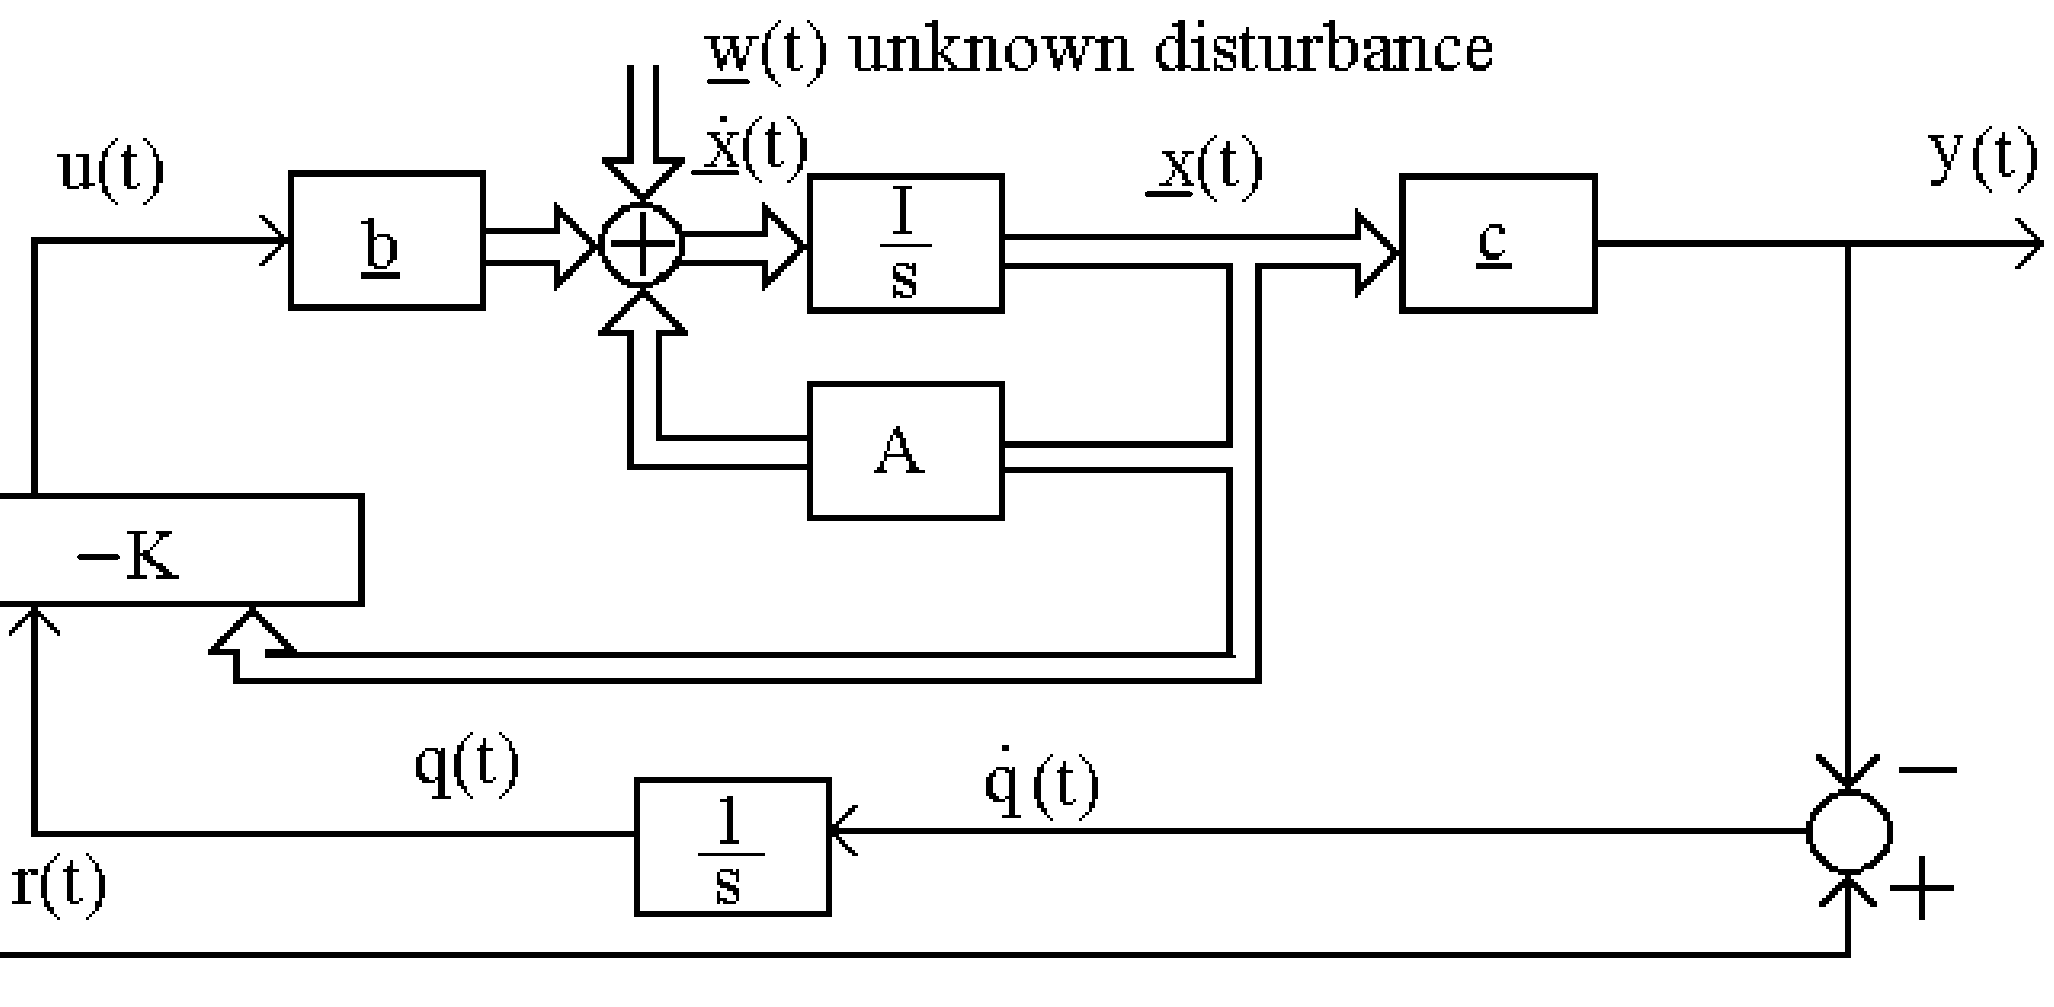
\includegraphics[width=\linewidth]{CTSIntegralTracking.png}
%\end{minipage}
\textbf{Combined Observer-Controller}

Observer feedback: $l(y(t)-c\tilde{x}(t))$,

Feedback control signal $u(t)=-K\tilde{x}(t)+v(t)$ \hfill \break 
Observation error: $\dot{e}(t)=(A-lc)e(t)$
$\det \begin{bmatrix}sI-A & bK \\
-lc & sI-A+lc+bK
\end{bmatrix} \\ =\det(sI-A+bk)\det(sI-A+lc)$
$\begin{bmatrix}
\dot{x}(t) \\
\dot{\tilde{x}}(t)
\end{bmatrix}= \begin{bmatrix}
A  & -bK \\
lc & A-lc-bK
\end{bmatrix}\begin{bmatrix}
x(t) \\
{\tilde{x}}(t)
\end{bmatrix}+
\begin{bmatrix}
b \\ b
\end{bmatrix} v(t) \quad 
\begin{bmatrix}
x(t_0) \\ \tilde{x}(t_0)
\end{bmatrix}=
\begin{bmatrix}
x_0 \\ \tilde{x}_0
\end{bmatrix}
$
\vspace{0.1 cm}
Quad Form: $ax^2+bx+c=0 \quad x= \frac{-b \pm \sqrt{b^2-4ac}}{2a}$,
Steady-state error is defined as the difference between the input (command) and the output of a system in the limit as time goes to infinity. $x_1(1)=x_2(0)$.
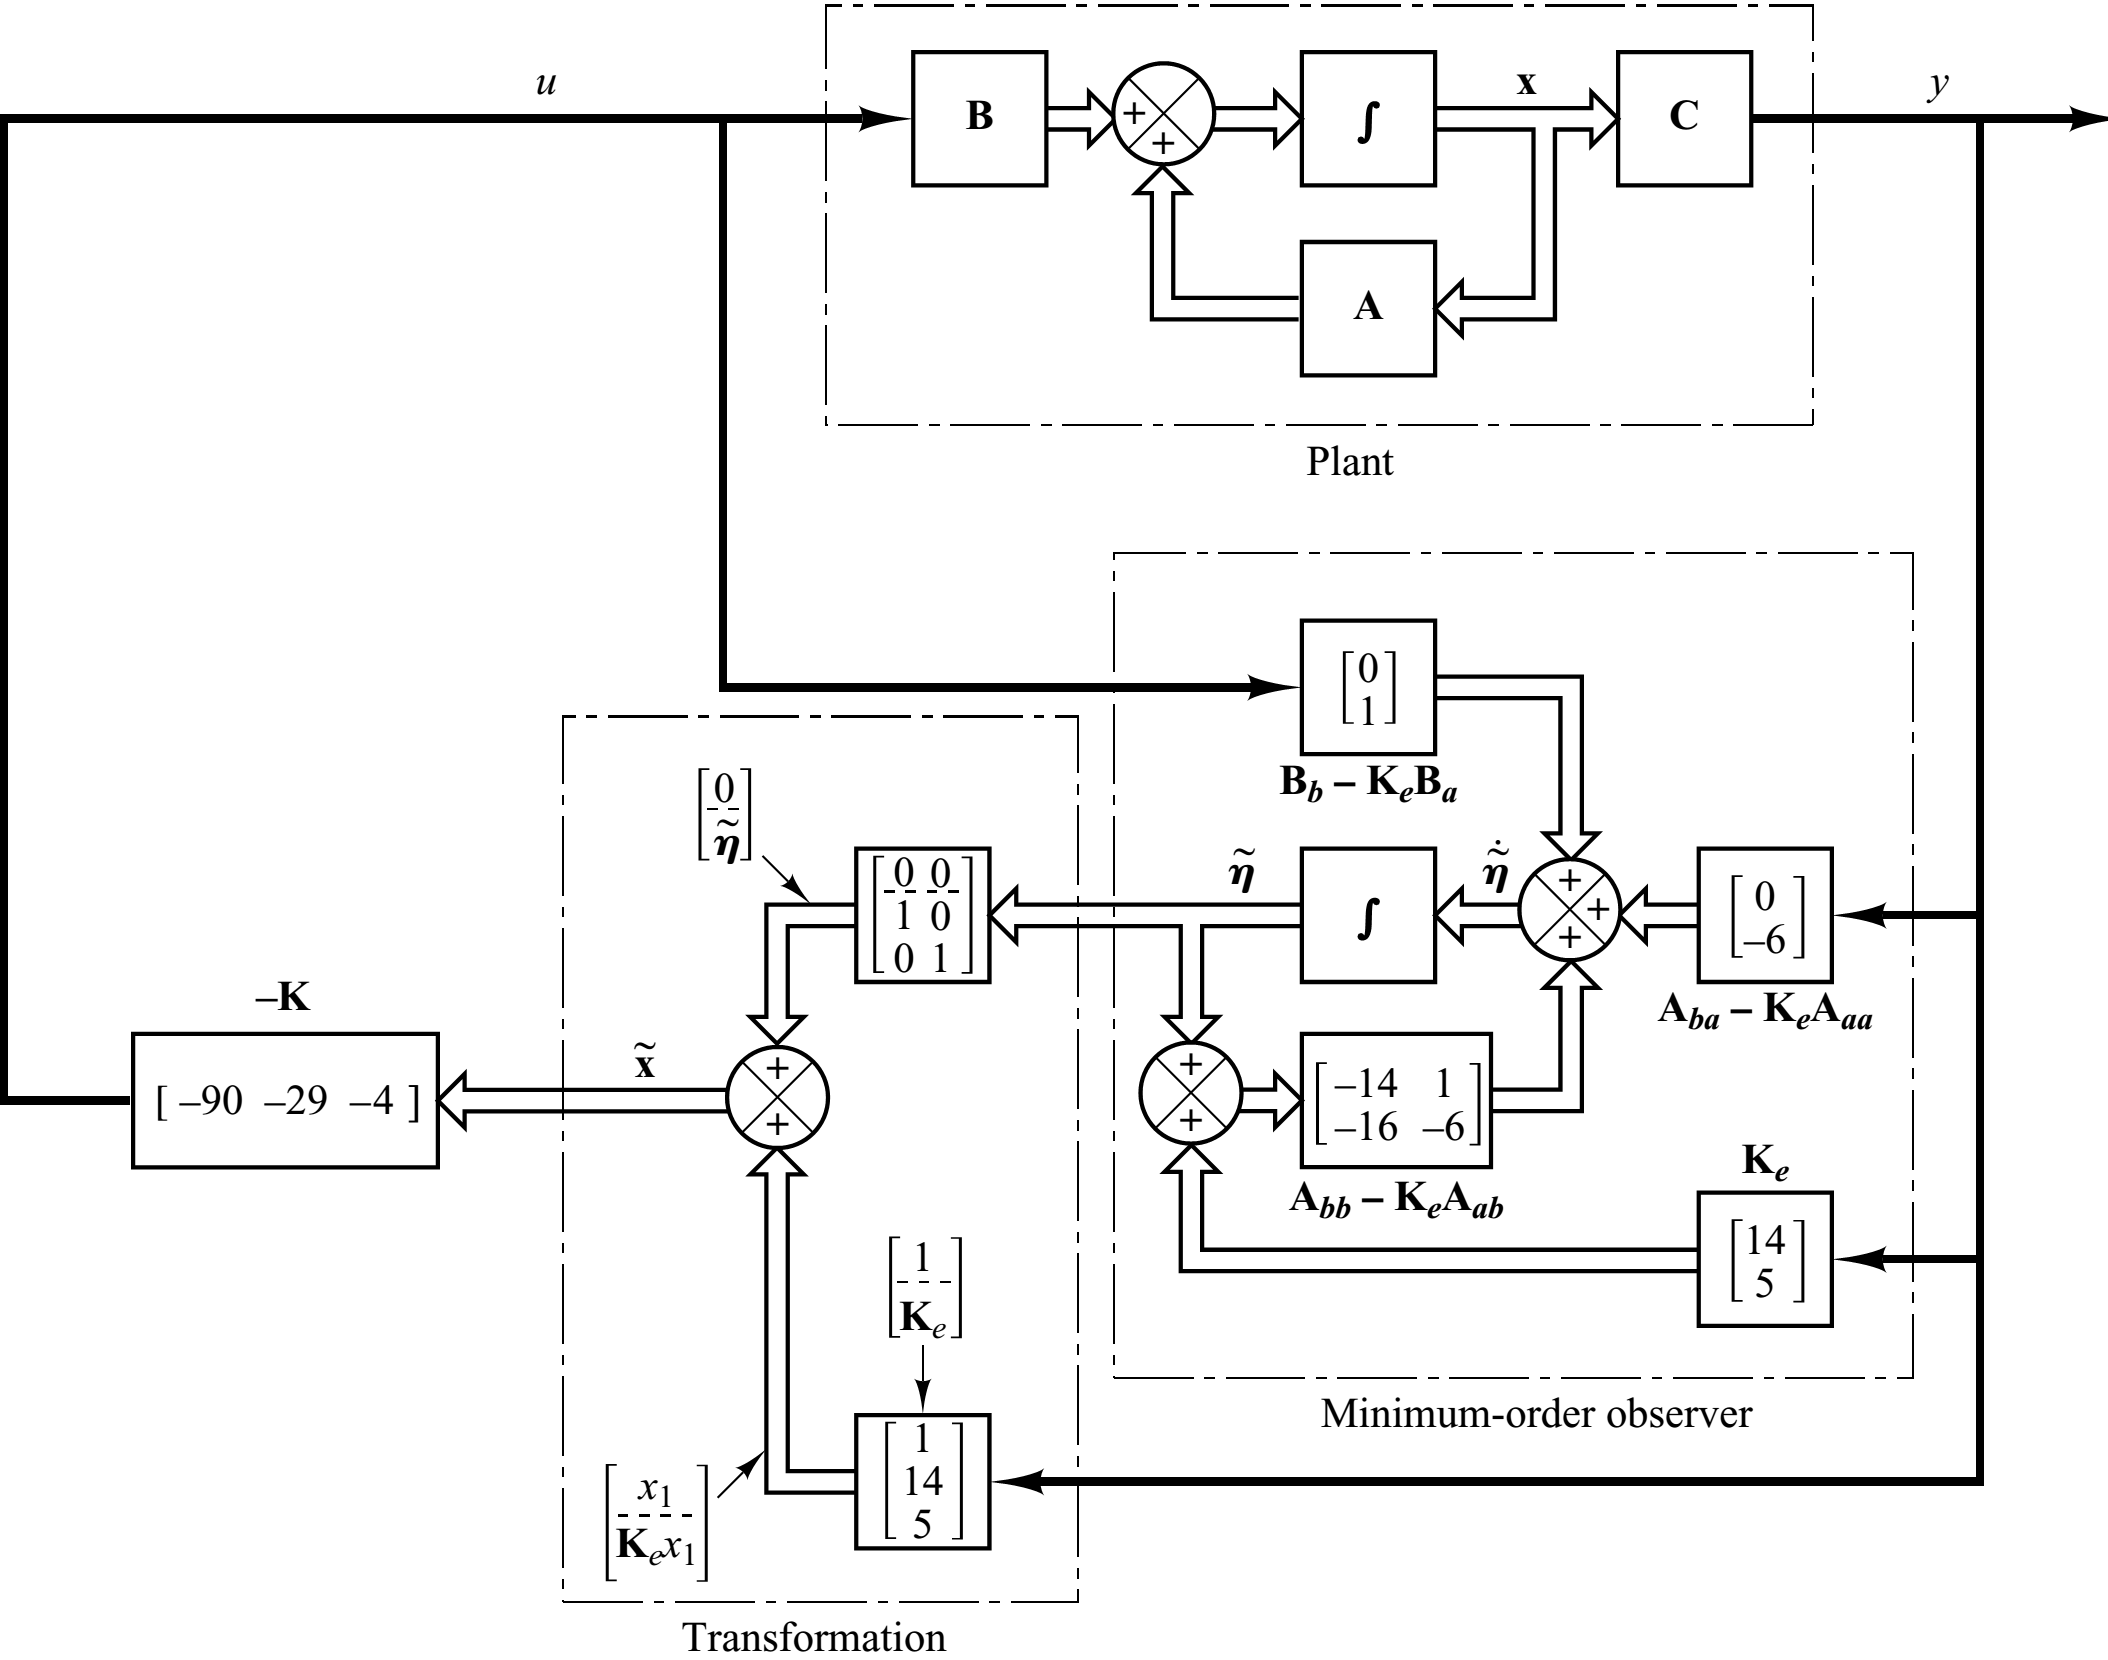
\includegraphics[width=\linewidth]{fullEstimateobs.png}
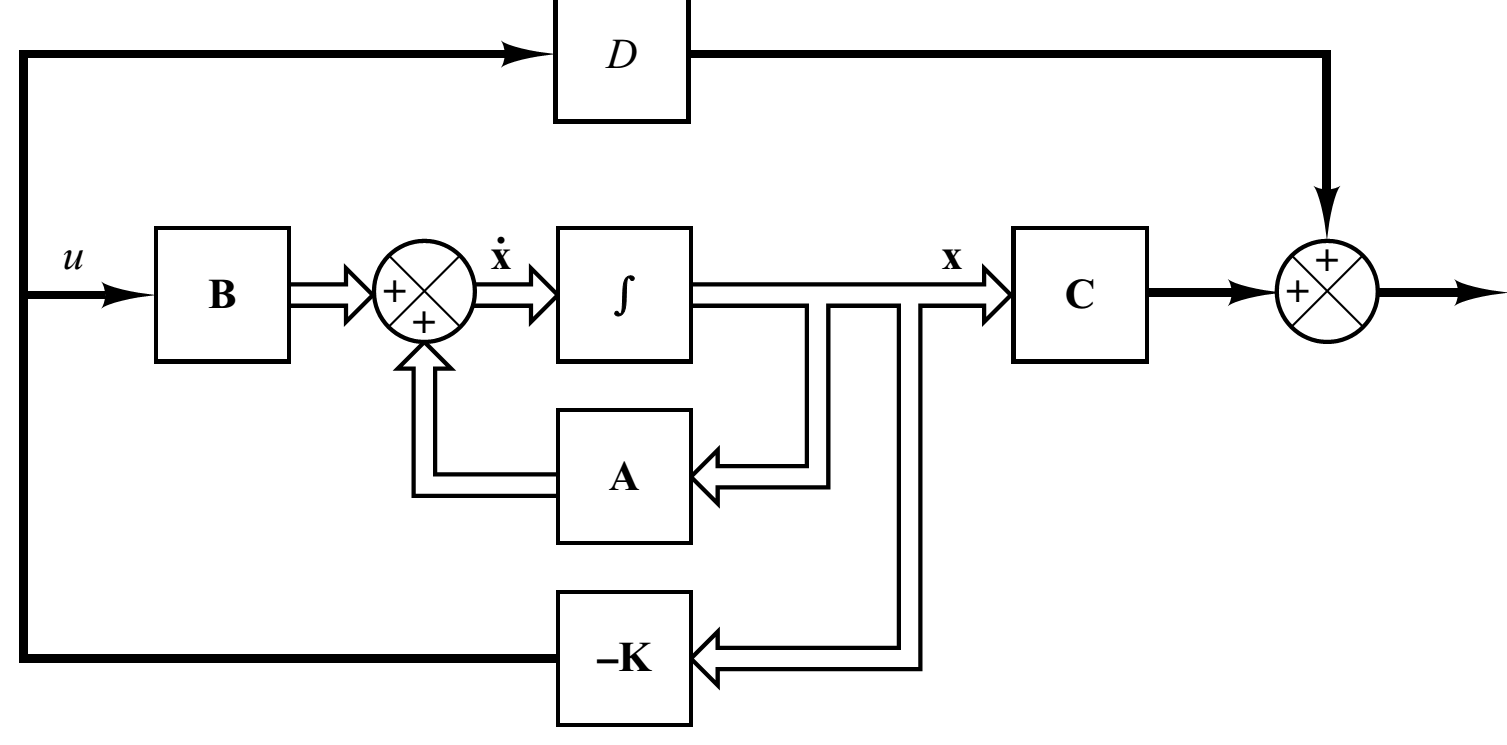
\includegraphics[width=\linewidth]{keFeedback.png}
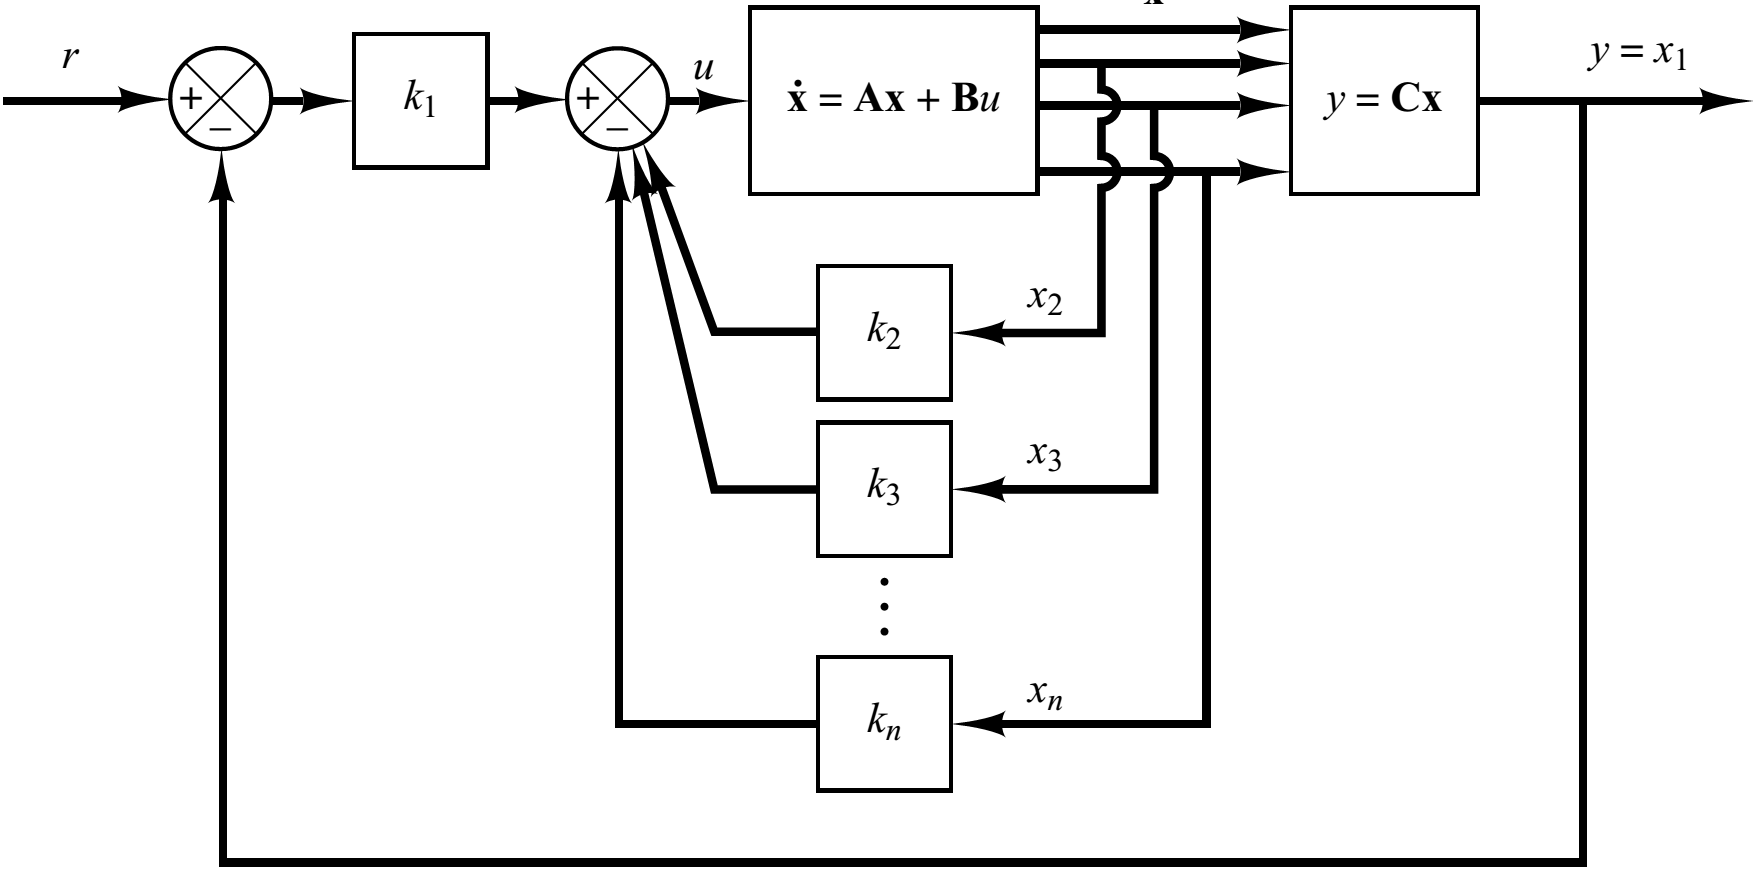
\includegraphics[width=\linewidth]{whyNot.png}
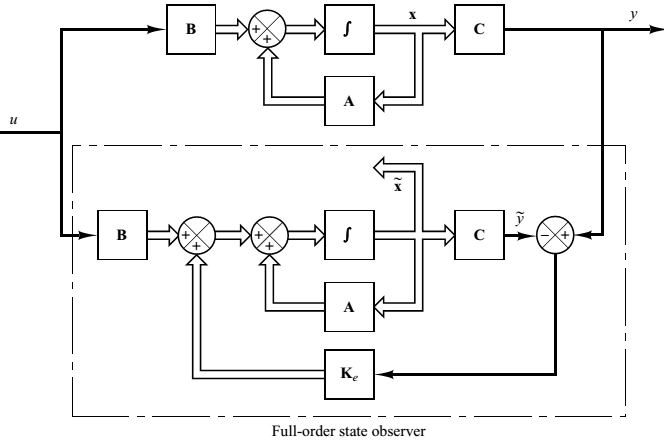
\includegraphics[width=\linewidth]{full-state-obs.png}
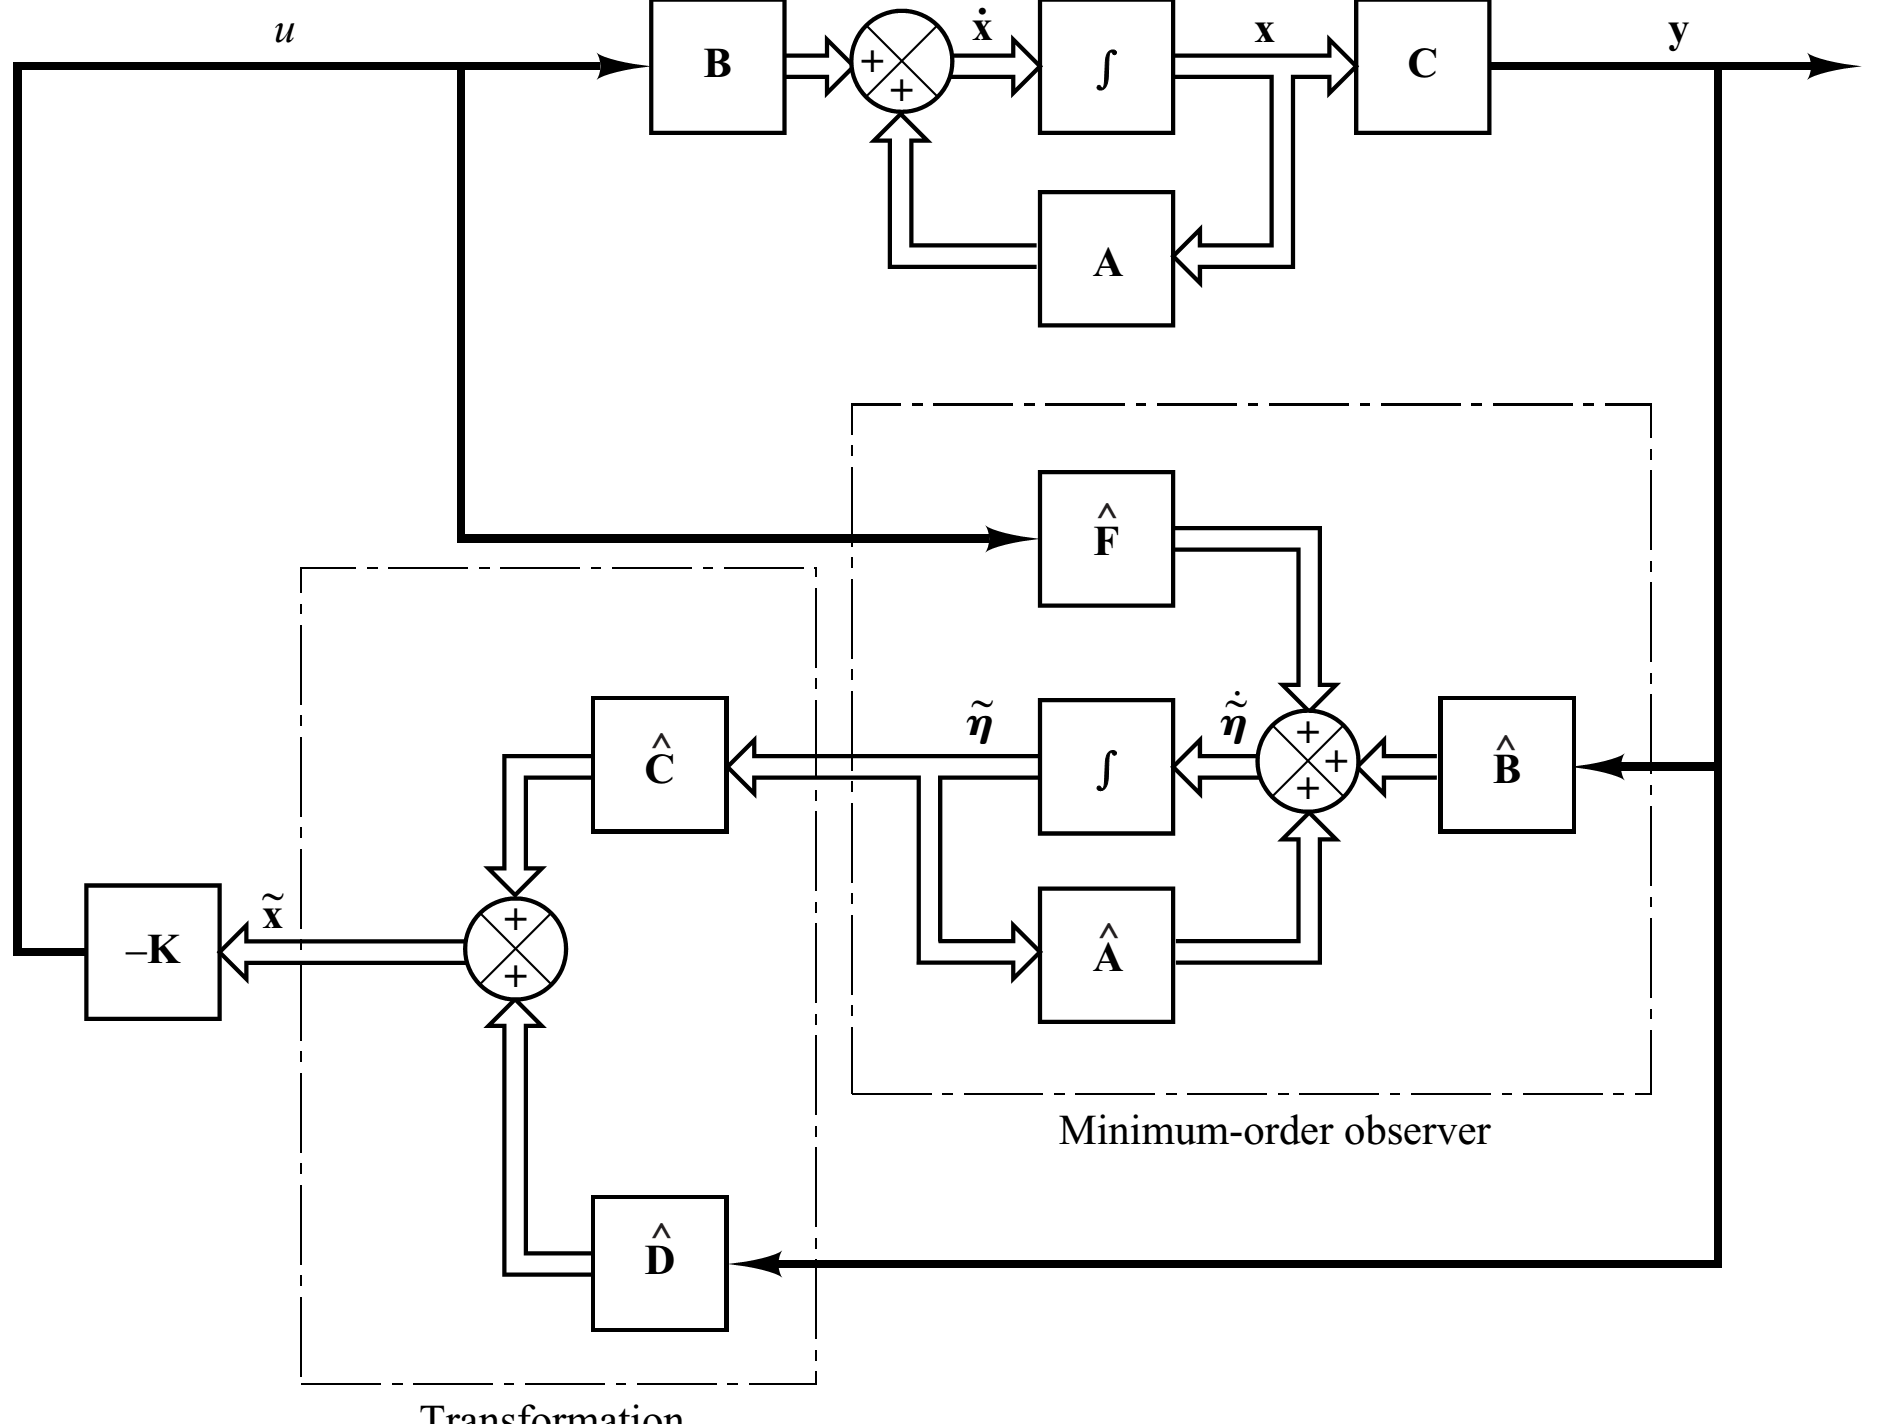
\includegraphics[width=\linewidth]{min-order-observer.png}




\subsection{Stability Test for Digital Systems}

\textbf{Jury-Marden Table Uses function P of z} \newline
%\vspace*{-0.25cm}
\begin{align*}
& b_k = \det \begin{bmatrix}
a_n & a_{n-1-k} \\
a_0 & a_{k+1}
\end{bmatrix} \\
& k = 0,1,  \cdots n-1 \\
& c_k = \det \begin{bmatrix}
b_{n-1} & b_{n-2-k} \\
b_0 & b_{k+1}
\end{bmatrix} \\
& k = 0,1,  \cdots n-1 \\
& q_k = \det \begin{bmatrix}
p_{3} & p_{2-k} \\
p_0 & p_{k+1}
\end{bmatrix} \\
& k =0,1,2
\end{align*}

\begin{tabular}{llllllll}
	\cline{1-5}
	Row & $z^0$     & $z^1$     & $z^2$     &          & $z^{n-2}$ & $z^{n-1}$ & $z^n$ \\ %\cline{1-5}
	1   & $a_n$     & $a_{n-1}$ & $a_{n-2}$ & $\cdots$ & $a_2$     & $a_1$     & $a_0$ \\
	2   & $a_0$     & $a_1$     & $a_2$     & $\cdots$ & $a_{n-2}$ & $a_{n-1}$ & $a_n$ \\
	3   & $b_{n-1}$ & $b_{n-2}$ & $b_{n-3}$ & $\cdots$ & $b_1$     & $b_0$     &       \\ %\cline{1-5}
	4   & $b_0$     & $b_1$     & $b_2$     & $\cdots$ & $b_{n-2}$ & $b_{n-1}$ &       \\
	5   & $c_{n-2}$ & $c_{n-3}$ & $c_{n-4}$ & $\cdots$ & $c_0$     &           &       \\
	6   & $c_0$     & $c_1$     & $c_2$     & $\cdots$ & $c_{n-2}$ &           &      \\
	2n-5& $p_3$ & $p_2$ & $p_1$ & $p_0$ & & & \\
	2n-4& $p_0$ & $p_1$ & $p_2$ & $p_3$ & & & \\
	2n-3& $q_2$ & $q_1$ & $q_0$ & & & & 
\end{tabular}

\begin{align*}
& P(z) = a_0z^n+a_1z^{n-1} + \cdots + a_{n-1}z+a_n \quad G(z)= \frac{A(z)}{P(z)} \\
& \text{Stability Condition:} \quad P(z) \neq 0 \quad |z| \geq 1 \quad (\text{Draw Unit Circle to test stability})\\
& \text{Routh-Stability in Digital Domain: } s = \frac{z+1}{z-1} \quad z=\frac{s+1}{s-1}
\end{align*}


\begin{align*}
& G(z) = \mathcal{Z} \left\{\left(\frac{1-e^{-s}}{s}\right) \left[ \frac{1}{s+1}\right] \left[\frac{1}{s}\right] \right\} \rightarrow G_1(z) = (1-z^{-1})\mathcal{Z} \left\{ \frac{1}{s^2(s+1)} \right\}
\end{align*}

All first-column elements of the Routh array are to be of the same sign. $a_0s^n + a_1s^{n-1}+ \cdots + a{n-1} s + a_n = 0$, first row is even entries $a_0$, $a_2$, next row is $a_1$, $a_2$, b entries are the same are jury-marden table.


\subsection{Z-transform}



\begin{tabular}{c c}
	$\mathcal{Z} \left\{ f_1(t) \pm f_2(t) \right\}=F_1(z)+F_2(z)$ & Addition\\
	$\mathcal{Z} \left\{ af(t) \right\}= aF(z)$ & Multiplication by a Constant \\
	$\mathcal{Z} \left\{ f(t-nT) \right\}=z^{-n}F(z)$ & Shifting \\
	$\mathcal{Z} \left\{ f(t+kT) \right\}=z^{k}F(z)-z^{k}f(0)- \cdots - z f(kT-T)$ & Shifting (cont'd) \\
	$\mathcal{Z} \left\{ e^{\mp at} f(t) \right\}=F(ze^{\pm at})$ & Complex Translation \\
	$\lim_{k \rightarrow \infty} f(kT)= \lim_{z \rightarrow 0}F(z)$ & Initial Value Theorem \\ 
	If $(1-z^{-1})F(z)$ has all singularities inside unit disk $|z|=1$, then & Final Value Theorem \\
	$\lim_{k \rightarrow \infty} f(kT) = \lim_{z \rightarrow 1} (1-z^{-1})F(z)$ & \\
	$\mathcal{Z} \left\{ \frac{\partial}{\partial a} f(t,a) \right\} = \frac{\partial}{\partial a} F(z,a)$ & Partial differentiation
\end{tabular}


\end{document}
